\documentclass[../vs-script-first-v01.tex]{subfiles}
\graphicspath{{\subfix{../}}}
\begin{document}


\section{Architektur}
In diesem Kapitel werden die Grundlagen behandelt, um die unterschiedlichen Formen der Realisierung von verteilten Systemen zu klassifizieren und einordnen zu können. Diese Diskussion sagt noch nichts über die reale Umsetzung aus, bietet aber den Einstiegspunkt in diese. Es wird darauf eingegangen, welche Vorkenntnisse notwendig sind und welche Ziele mit den Architekturansätzen erreicht werden sollen. 
\subsection{Grundlagen für die Realisierung}

Um sich den Freiheitsgraden der Realisierung von Verteilten Systemen bewusst zu werden, kann man sich im ersten Schritt noch einmal die grundsätzliche Architektur einer Recheneinheit vor Augen führen, die in diesem Kontext immer für die Problemlösung herangezogen werden (Wenngleich andere Ansätze auch denkbar sind). Typische Referenzen in diesem Fall sind die Harvard- oder die von-Neumann Architektur. 
\\\\
Die Harvard-Architektur und die von-Neumann-Architektur sind beides grundlegende Architekturen für die Gestaltung von Computern und digitalen Rechensystemen. Beide Architekturen haben gemeinsam, dass sie die Grundlagen für die Funktionsweise moderner Computer bilden und auf der Verwendung von Binärcode und elektronischen Komponenten basieren.

Eine wichtige Unterscheidung besteht natürlich darin, dass die von Neumann-Architektur eine gemeinsame Speicherarchitektur hat, in der sowohl Anweisungen als auch Daten in einem gemeinsamen Speicher gespeichert werden. Die Harvard-Architektur hingegen verwendet getrennte Speicher für Anweisungen und Daten, was zu einem schnelleren Zugriff auf beide Arten von Informationen führen kann.
\\\\
Wie es auch sei,  beide Architekturen bieten einfach gesprochen ein Befehlssatz/Instruction Set Architecture (ISA), welches sich auf die spezifischen Anweisungen und Befehle bezieht, die ein Prozessor oder ein digitales Rechensystem ausführen kann, sowie die Möglichkeit der Datenrepräsentation, auf denen diese Anweisungen und Befehle basieren oder ausgeführt werden.
\\\\
Somit ergibt sich, das in einem Verteilten System\footnote{welches mindestens aus zwei Systemen besteht} die Notwendigkeit die Befehle oder Anweisung für eine kooperative Lösungsstrategie über ein Netzwerk zu addressieren. Die Herangehensweise an diese Herausforderung kann unterschiedlich interpritiert werden. Um die Strategien besser beurteilen zu können sollen zunächst die Zerlegungsmethoden und generellen Kommunikationsformen an den Schnittstellen diskutiert werden. 

\subsubsection{Funktionale vs. ressourcenorientierte Zerlegung}

In der Softwarearchitektur gibt es mehrere Teile-und-herrsche-Ansätze, um komplexe Systeme zu entwickeln und zu verwalten. Zunächst soll aber der Fokus auf eine Einteilung in zwei rudimentäre Ansätze gelegt werden:
\importantvs{
\begin{itemize} 
\item Funktional
\item Ressourcenorientiert
\end{itemize}
}
Bei der funktionalen Zerlegung wird das System in kleinere, im besten Fall atomare, Funktionen/Prozeduren zerlegt, die jeweils auf eine bestimmte Aufgabe spezialisiert sind. Die Idee ist, dass jede Funkion unabhängig von den anderen funktioniert, um das System als Ganzes zu unterstützen. Beispielhaft könnte das eine Funktion sein, dass die Sortierung von Zahlen übernimmt, aber auch eine Funktion für die Filterung oder Suche. Die funktionale Zerlegung zielt darauf ab, die Komplexität des Systems zu reduzieren, indem es in kleinere, leichter handhabbare Teile aufgeteilt wird. 
Einfach gesprochen werden folgend disjunkte Funktionen bestimmt, versucht diese generisch zu erfassen und abstrahiert zu beschreiben. Eine Unterscheidung in \enquote{Funktionale}, \enquote{Deklarative} oder \enquote{Objektorientierte} Programmierung soll zu diesem Zweitpunkt noch nicht getroffen werden, da es auch in einem Verteilten System notwendig sein wird, unterschiedliche Programmierungsansätze miteinander zu verbinden. 
Zudem kann zu diesem Zeitpunkt auch mal festgestellt werden, dass die Auswahl der Sprache für die Lösung eines bestimmten Problems keine Rolle spielt, wenn alle beteiligten Sprachen Turing-vollständig sind. Das bedeutet, dass jede dieser Sprachen in der Lage ist, jede denkbare Berechnung durchzuführen, solange genügend Zeit und Speicherplatz zur Verfügung stehen.
\\\\
Richten wir weiter den Blick zunächst weiter auf Funnktionen und Prozesse. Für die Beschreibung von Funktionen/Prozessen gibt es eine recht generische Form, die über jeden Architekurtyp und jeder Sprache relativ konstant bleibt.
\importantvs{
\begin{itemize} 
\item Funktionssignatur 
\item Funktionssemantik (Definition)
\end{itemize}
}
Ein Beispiel für die Formulierung einer Funktionssignatur in Pseudocode könnte für die Addition zweier Werte in dieser Form beschrieben werden:
\begin{lstlisting}[caption={Funktionssignatur},captionpos=b,label={lst:signatur}]
    function sum(a: int, b: int) -> int;
\end{lstlisting}
Die Funktionssignatur in Listing \ref{lst:signatur} gibt an, dass die Funktion \enquote{sum} zwei Parameter vom Typ \enquote{int} erwartet und einen Rückgabewert vom Typ \enquote{int} liefert. Einige der wichtigsten Informationen, die in einer Funktionssemantik enthalten sein können, sind:
\begin{itemize} 
\item Der Name der Funktion:\\ Dies gibt an, wie die Funktion genannt wird und welche Funktion sie ausführt.
\item Die Parameter der Funktion:\\ Dies beschreibt, welche Eingabe die Funktion erwartet und welche Bedeutung die einzelnen Parameter haben.
\item Der Rückgabewert der Funktion:\\ Dies beschreibt, welche Ausgabe die Funktion liefert und welche Bedeutung der Rückgabewert hat.
\item Die Bedingungen und Einschränkungen:\\ Dies beschreibt, welche Bedingungen erfüllt sein müssen, damit die Funktion korrekt ausgeführt wird, und welche Einschränkungen es bei der Verwendung der Funktion gibt.
\item Die Ausführungslogik:\\ Dies beschreibt, wie die Funktion ausgeführt wird, welche Schritte dabei durchlaufen werden und welche Algorithmen verwendet werden.
\item Die Fehlerbehandlung:\\ Dies beschreibt, wie die Funktion mit Fehlern und Ausnahmen umgeht und welche Ausnahmen auftreten können.
\end{itemize} 
Die spezifischen Informationen, die in einer Funktionssemantik enthalten sind, hängen von der Art der Funktion und den Anforderungen der Anwendung ab, dennoch beschreibt auch die geringste Variante die Schnittstelle zu einem Teil des Befehlssatzes der zugrunde liegenden Architektur. 
\\\\
Die Funktionssemantik beschreibt die Bedeutung und den Zweck einer Funktion, nicht aber zwingend die Umsetzung auf dem Befehlssatz der Architektur. Sie beschreibt, was die Funktion tut und wie sie ausgeführt wird. Die Funktionssemantik kann in Form von Kommentaren, Dokumentation oder einfach durch den Code selbst ausgedrückt werden.
\begin{lstlisting}[caption={Funktionssemantik},captionpos=b,label={lst:semantik}]
    function sum(a: int, b: int) -> int {
        return a + b;
    }
\end{lstlisting}
Listing \ref{lst:semantik} beschreibt, dass die Funktion \enquote{sum} die beiden Parameter \enquote{a} und \enquote{b} addiert und das Ergebnis zurückgibt. In diesem Beispiel wird die Funktionssemantik durch den Code selbst ausgedrückt. Sind systematisch und vollständig alle atomaren Funktionen mit Funktionssignatur und Funktionssemantik in der Anforderungsanalyse und im Design bestimmt, kann aus der Summe aller Funktionen mit einer Funktionskomposition das gesamte System als die Summe aller Funktionen erstellt werden. Bei der Funktionskomposition werden Funktionen kombiniert, um komplexe Aufgaben zu erfüllen. Das Ergebnis der Funktionskomposition kann die erwartete Applikation sein, oder ein Teil des Gesamtdienstes (Service), der von dem Gesamtsystem erbracht werden soll. 
\\\\
Im Gegensatz dazu bezieht sich die ressourcenorientierte Zerlegung auf die Zerlegung des Systems in kleinere, auf Ressourcen orientierte Sicht. Die Idee ist, dass jede Einheit auf eine bestimmte Ressource spezialisiert ist und sie effizient nutzen kann, um das System als Ganzes zu unterstützen indem eine Schnittstelle zu der Ressource angeboten wird. Die Eigenschaften der Ressourcen werden typischerweise über ein reduziertes Set von Funktionen manipuliert.  In Bezug auf die ressourceorientierte Zerlegung ist CRUD\index{CRUD} ein wichtiger Teil des Entwurfsprozesses, da es die grundlegenden Operationen definiert, die auf Ressourcen angewendet werden können. Jede Ressource wird normalerweise mit einer oder mehreren der CRUD-Operationen verbunden sein.
Unter CRUD versteht man üblicherweise folgende Funktionen:

\begin{itemize}
\item \textbf{Create}: Erstellen oder Hinzufügen von neuen Daten in der Anwendung. Zum Beispiel kann ein Benutzer ein neues Konto erstellen oder ein Administrator kann einen neuen Datensatz hinzufügen.

\item \textbf{Read}: Lesen oder Abrufen von vorhandenen Daten aus der Anwendung. Zum Beispiel kann ein Benutzer seine Profilinformationen abrufen oder ein Mitarbeiter kann einen Bericht lesen.

\item \textbf{Update}: Aktualisieren oder Ändern von vorhandenen Daten in der Anwendung. Zum Beispiel kann ein Benutzer seine Profilinformationen aktualisieren oder ein Administrator kann die Kontaktinformationen eines Kunden ändern.

\item \textbf{Delete}: Löschen oder Entfernen von vorhandenen Daten aus der Anwendung. Zum Beispiel kann ein Benutzer sein Konto löschen oder ein Administrator kann einen ungenutzten Datensatz entfernen.
\end{itemize}
Die Schnittstelle einer Ressource muss nicht auf CRUD Funktionen reduziert sein, oder sie exakt in dieser Form umsetzen, aber wichtig ist dieses Konzept allemal.
\\\\

\begin{figure}[ht!]
  \centering
  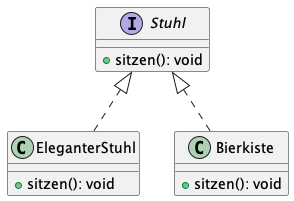
\includegraphics[width=0.4\textwidth]{fig/uml/stuhl-function.png}
  \caption{Funktionale Zerlegung mit Interface}
  \label{fig:stuhl-f}
\end{figure}

\begin{figure}[ht!]
  \centering
  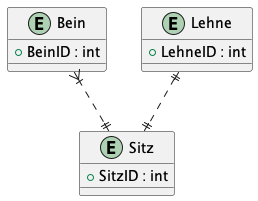
\includegraphics[width=0.4\textwidth]{fig/uml/stuhl-resourcen.png}
  \caption{Ressourcen-orientierte Zerlegung mit Relation}
  \label{fig:stuhl-r}
\end{figure}
Um den Unterschied der Ansätze nochmal zu verdeutlichen soll die Analogie der \enquote{Zerlegung eines Stuhls} als Sitzgelegenheit herangezogen werden. Wo bei der funktionalen Zerlegung die Suche nach einer Funktionen, wie das \enquote{Sitzen} im Vordergrund steht, und bei der ressourcenorientierten Zerlegung die Identifikation der einzlenen Ressourcen, wie (Stuhl-)Bein, Sitz(-fläche) oder (Rücken-)Lehne. Umgesetzt in ein Designentwurf für die funktionale Zerlegung ergibt sich beispielhaft in einer objektorientierten Sprache folgender der in dem Diagramm\ref{fig:stuhl-f} zu erkenne ist. 

In diesem Beispiel ist es wichtig zu erkennen, dass das Design mit der funktionalen Zerlegung auch seine Schwächen hat. Auch wenn eine korrekte Funktionssignatur bestimmt wurde, kann sich hinter dem Interface der realen Umsetzung dennoch eine nicht zu erwartende Umsetzung verbergen. In diesem  Beispiel wird beim Versuch sich zu setzen nicht nur ein eleganter Stuhl zu erwarten sein, sondern es kann auch eine Bierkiste die Sitzmöglichkeit repräsentieren. Diese Möglicheiten der Polymorphie eröffnet Chancen und Risiken.  
\\\\
Die ressourcenorientierte Zerlegung ist dahingehend intuitiver (siehe Abbildung \ref{fig:stuhl-r}, da ein System in seine einzelnen Ressourcen zerlegt wird, wobei diese eindeutig identifizierbar sein müssen. Auf diese Weise können diese Ressourcen als Entitäten Beziehungen zueinander aufbauen, welche wiederum mit weiteren Eigenschaften belegt werden können. In der korrekten Umsetzung ergibt sich so ein gutes Bild des Gesamtsystems. Die Gefahr besteht jedoch darin, dass die Ressourcen und deren Attribute nicht genau genug bestimmt werden oder die Beziehungen falsch beschrieben sind. In der hier benannten Analogie kann der Bausatz eines Stuhls auch auf eine Art und Weise beschrieben werden, dass die Lehne an den Beinen montiert ist und somit trotz identifizierter Ressourcen nicht den Dienst eines Stuhles, zumindest wie er erwartet wird, erfüllen kann.

Der geneigte Leser könnte als Übung hinterfragen, wie die Umsetzung eines Schachspiels in der funktionalen Zerlegung beschrieben werden könnte und wie dies in der ressourcenorientierten Zerlegung aussehen würde. So ergeben sich beispielhaft die Optionen, dass das Spielbrett sowohl in der objektorientierten Sprache durch eine Klasse mit Methoden ausgedrückt wird, die das Brett und die Spielregeln verwaltet, oder als Datenbankressource mit der gleichen Aufgabe.

Bei der Datenbank-Ressource werden die Spielzüge mit dem CRUD Interface realisiert. Spielregeln könnten durch Datenbank-Trigger erfasst werden. Ein Datenbank-Trigger ist ein spezielles Programm oder Skript, das  automatisch ausgeführt wird, wenn bestimmte Änderungen an einer Datenbanktabelle oder -sicht vorgenommen werden. Der Trigger wird auf eine bestimmte Aktion (z.B. INSERT, UPDATE oder DELETE) festgelegt und kann verwendet werden, um eine Reihe von Aufgaben oder Maßnahmen auszuführen, wenn diese Aktion auftritt.

\noindent\begin{minipage}{\textwidth}
\begin{lstlisting}[caption={Schachbrett - Objektorientiert},captionpos=b,label={lst:schachbrett-oo}]
public class ChessBoard {
    private Piece[][] board;

    public ChessBoard() {
        this.board = new Piece[8][8];
        // Initialize the board with the starting positions of pieces
        // e.g. add new Piece(PieceType.ROOK, Color.WHITE) to board[0][0] for the white rook in the top-left corner.
    }

    public Piece getPiece(int row, int col) {
        return board[row][col];
    }

    public void setPiece(int row, int col, Piece piece) {
        board[row][col] = piece;
    }

    // Other methods for checking if a move is valid, getting a list of possible moves, etc.
}
\end{lstlisting}
\end{minipage}

Die Wahl der richtigen Methode hängt von verschiedenen Faktoren ab, wie z.B. der Komplexität des Systems, der Art der Aufgaben, die ausgeführt werden müssen, und den verfügbaren Ressourcen.

Für die Zerlegung in einem verteilten System hat bereits die Auswahl der grundlegenden Strategie der Zerlegung einen hohen Einfluss. Die Schnittstellen der Systeme ändern sich dadurch und damit auch die notwendige Kommunikation und die Datenrepräsentation in den Systemen.\footnote{Eine weitere Art der Diskussion: \url{https://medium.com/double-pointer/system-design-interview-a-two-player-online-chess-game-4a150ad8ea78} }

\noindent\begin{minipage}{\textwidth}
\begin{lstlisting}[caption={Schachbrett - Datenbank},captionpos=b,label={lst:schachbrett-datenbank}]

CREATE TABLE ChessBoard (
    id INT PRIMARY KEY,
    row INT,
    col INT,
    pieceType VARCHAR(10),
    pieceColor VARCHAR(5)
);
\end{lstlisting}
\end{minipage}


\subsubsection{Datenseparation}

Die Datenseparation in verteilten Systemen bezieht sich auf den Prozess, bei dem Daten auf mehrere Knoten in einem Netzwerk verteilt werden, um die Leistung, Skalierbarkeit und Zuverlässigkeit des Systems zu verbessern. Dies wird typischerweise durch die Aufteilung von Daten in kleine Teile und deren Verteilung auf verschiedene Knoten oder Server im Netzwerk erreicht.
Es gibt verschiedene Möglichkeiten, Daten in verteilten Systemen zu separieren, einschließlich:
\begin{itemize}
\item \textbf{Horizontale Partitionierung}\index{Partitionierung}\index{horizontal}: Hierbei wird eine Tabelle in mehrere kleinere Tabellen aufgeteilt und jede Teilung wird auf einem separaten Server gespeichert. Zum Beispiel könnte man Kundeninformationen basierend auf Regionen oder Alphabeten auf verschiedene Server verteilen.

Ein Beispiel für ein Unternehmen, das Horizontale Partitionierung einsetzt, ist Facebook. Facebook speichert seine Daten in einer horizontal partitionierten Datenbank, bei der jede Tabelle in mehrere Teilbereiche aufgeteilt wird, wobei jeder Teilbereich nur bestimmte Zeilen enthält. Dies ermöglicht es Facebook, die Last auf mehrere Datenbankserver zu verteilen und eine bessere Skalierbarkeit zu erreichen. Wenn ein Benutzer beispielsweise eine Suche durchführt, kann Facebook nur die benötigten Zeilen abfragen und somit eine schnellere Antwortzeit erzielen.
\item \textbf{Vertikale Partitionierung}\index{Partitionierung}\index{vertikal}: Hierbei werden bestimmte Spalten einer Tabelle auf verschiedene Server verteilt. Zum Beispiel könnten personenbezogene Daten (Name, Geburtsdatum, Adresse usw.) auf einem Server gespeichert werden, während andere Daten wie Kontaktinformationen auf einem anderen Server gespeichert werden.

Ein Beispiel für eine Anwendung, die Vertikale Partitionierung einsetzt, ist die Online-Shop-Plattform Amazon. Amazon speichert seine Daten in einer vertikal partitionierten Datenbank, bei der jede Tabelle in mehrere Teilbereiche aufgeteilt wird, wobei jeder Teilbereich nur bestimmte Spalten enthält. Wenn ein Benutzer beispielsweise eine Suche nach einem bestimmten Produkt durchführt, kann Amazon nur die benötigten Spalten abfragen und somit eine schnellere Antwortzeit erzielen.

Ein weiteres Beispiel ist LinkedIn, die auch Vertikale Partitionierung nutzen, um ihre Datenbank effizienter zu gestalten. LinkedIn speichert ihre Nutzerdaten in verschiedenen Datenbanken, die jeweils auf bestimmte Anwendungen und Funktionen zugeschnitten sind. Dadurch können sie die Ladezeiten reduzieren und eine bessere Skalierbarkeit erreichen.
\item \textbf{Sharding}\index{Sharding}: Hierbei wird die Datenbank in kleine, unabhängige Teile aufgeteilt, die auf verschiedenen Servern gespeichert werden. Dies ermöglicht eine horizontale Skalierung und verbessert die Leistung des Systems. Sharding ist eine Art der horizontalen Partitionierung, die Daten auf der Grundlage eines Sharding-Schlüssels aufteilt.

Slack ist ein Beispiel für eine Anwendung, die eine Form des Sharding verwendet, um ihre Datenbankleistung zu skalieren. Sharding ist eine Technik, bei der eine Datenbank in mehrere Teilbereiche aufgeteilt wird, die als \enquote{Shards} bezeichnet werden. Jeder Shard enthält einen Teil der Daten, so dass die Datenbank effizienter und schneller durchsucht werden kann.

In Slack wird Sharding verwendet, um die Benutzerdaten zu partitionieren. Das bedeutet, dass die Daten der Benutzer in mehrere Shards aufgeteilt werden, um die Last auf mehrere Datenbankserver zu verteilen. Jeder Shard ist dabei in der Lage, seine eigene Last zu verarbeiten und kann unabhängig von den anderen Shards skaliert werden. Dadurch kann Slack eine höhere Skalierbarkeit und eine bessere Leistung erzielen.
\item Daten-\textbf{Replikation}: Hierbei werden Daten auf mehreren Knoten im Netzwerk gespeichert, um Redundanz und Fehlertoleranz zu gewährleisten. Wenn ein Knoten ausfällt, kann ein anderer Knoten die Arbeit übernehmen und sicherstellen, dass das System weiterhin funktioniert.
\end{itemize}
Die Datenseparation in verteilten Systemen ist ein wichtiger Aspekt für die Skalierung und die Verfügbarkeit von Anwendungen. Durch die Verteilung von Daten auf mehrere Knoten im Netzwerk kann das System schnell auf Anforderungen reagieren und bietet eine hohe Verfügbarkeit, selbst wenn einzelne Knoten ausfallen.

\subsubsection{Schnittstellen zwischen den Entitäten}

Verteilte Systeme bestehen aus mehreren eigenständigen \enquote{nodes}, die über ein Netzwerk miteinander verbunden sind und gemeinsam arbeiten. Jede node repräsentiert eine Funktion oder eine Ressource, bzw. die Orchestrierung im funktionalen bzw. ressource-orientierten Ansatz. Unabhängig der Zerlegungsmethode müssen diese nodes miteinander kommunizieren, um Daten auszutauschen und ihre Arbeit zu koordinieren. Hier sind einige Gründe, warum verteilte Systeme Kommunikation benötigen:

\begin{itemize}
\item Datenaustausch: In verteilten Systemen müssen Daten zwischen verschiedenen Computern ausgetauscht werden, um eine gemeinsame Aufgabe zu erfüllen. Beispielsweise müssen Datenbanken in verschiedenen Computern synchronisiert werden, damit jeder Computer auf die aktuellste Version der Daten zugreifen kann.
\item Ressourcenmanagement: In verteilten Systemen können Ressourcen wie Speicher, Prozessoren und Netzwerkbandbreite auf verschiedene Computer verteilt werden. Um diese Ressourcen effektiv zu nutzen, müssen die Computer miteinander kommunizieren und Ressourcenanforderungen und -freigaben koordinieren.
\item Koordination: In verteilten Systemen müssen die Computer miteinander kommunizieren, um Aufgaben zu koordinieren. Beispielsweise können sie Nachrichten austauschen, um sicherzustellen, dass jeder Computer über den Fortschritt der Aufgabe informiert ist und seinen Teil der Arbeit erledigt.
\item Fehlererkennung und -behebung: In verteilten Systemen kann ein Computer ausfallen oder fehlerhaft arbeiten. Die verbleibenden Computer müssen miteinander kommunizieren, um den Fehler zu erkennen und die Arbeit neu zu verteilen oder den fehlerhaften Computer auszuschließen.
\item Skalierung: In verteilten Systemen kann die Anzahl der Computer erhöht werden, um die Leistung zu verbessern oder um mit einer höheren Last umzugehen. Um diese Skalierbarkeit zu erreichen, müssen die Computer miteinander kommunizieren und ihre Arbeit effektiv aufteilen.
\end{itemize}    

\textbf{Kommunikation ist in verteilten Systemen unerlässlich}, somit muss diskutiert werden, welche Art der Kommunikation Unterstützung findet. Zunächst müssen aber die Freiheitsgrade identifiziert werden. 
Eine wesentliche Unterscheidung ist synchron und asynchron. Dies bezieht sich auf die Art und Weise, wie Informationen zwischen Systemen oder Komponenten über ihre Schnittstellen (Interfaces) ausgetauscht werden. Hier sind die Unterschiede zwischen synchrone und asynchrone Kommunikation:

\begin{itemize} 
\item Synchrone\index{synchrone} Kommunikation bedeutet, dass die Kommunikation in (beinah) Echtzeit stattfindet, d.h. der Sender wartet auf eine Antwort des Empfängers, bevor er mit der nächsten Aktion fortfährt. Beispielsweise kann eine Anwendung eine Anforderung an eine Datenbank senden und auf die Antwort der Datenbank warten, bevor sie mit der Verarbeitung der nächsten Anforderung fortfährt. Bei synchroner Kommunikation kann das System oder die Anwendung nur dann fortfahren, wenn die Antwort vollständig ist.
\item Asynchrone\index{asynchrone} Kommunikation hingegen bedeutet, dass die Kommunikation asynchron oder zeitversetzt erfolgt, d.h. der Sender sendet eine Nachricht an den Empfänger, ohne auf eine sofortige Antwort zu warten. Der Empfänger verarbeitet die Nachricht dann und sendet eine Antwort zurück, wenn er bereit ist. Beispielsweise kann eine Anwendung eine Anforderung an einen Server senden und ohne auf eine Antwort zu warten, mit der Verarbeitung der nächsten Anforderung fortfahren. Die Antwort des Servers wird später empfangen, wenn sie verfügbar ist.
\end{itemize}  
Synchrone Kommunikation ist einfach zu implementieren und zu kontrollieren, da der Sender auf eine Antwort des Empfängers wartet, bevor er fortfährt. Es ist jedoch langsam, da der Sender auf die Antwort des Empfängers warten muss, bevor er weitere Aktionen ausführen kann.

Asynchrone Kommunikation hingegen ist schneller, da der Sender die nächste Aktion ausführen kann, ohne auf die Antwort des Empfängers zu warten. Es ist jedoch schwieriger zu implementieren und zu kontrollieren, da der Sender und Empfänger möglicherweise nicht synchronisiert sind und es zu Datenverlust oder Fehlern kommen kann. \textbf{Bereits zu diesem Zeitpunkt sollte festgestellt werden, dass ein Design mit asynchronen Aufrufen dennoch in Verteilten Systemen vorzuziehen ist}.
\\\\
Eine weitere Unterscheidung in der Kommunikation ist persistent\index{persistent} und transient\index{transient}. Persistente und transiente Kommunikation beziehen sich auf die Art und Weise, wie Daten in einem verteilten System übertragen werden und ob die Daten dauerhaft oder vorübergehend gespeichert werden.

Persistente Kommunikation bedeutet, dass die Daten, die zwischen den Systemen übertragen werden, dauerhaft gespeichert werden. Das bedeutet, dass die Daten im besten Fall auch nach einem Systemausfall oder einem Neustart des Systems noch verfügbar sind. Bei der persistenten Kommunikation wird die Datenübertragung oft über Protokolle wie das Transmission Control Protocol (TCP) abgewickelt, die sicherstellen, dass die Daten vollständig und fehlerfrei übertragen werden.

Transiente Kommunikation hingegen bedeutet, dass die Daten, die zwischen den Systemen uni- oder bidirektional übertragen werden, vorübergehend und nicht dauerhaft gespeichert werden. Das bedeutet, dass die Daten nach einem Systemausfall oder einem Neustart des Systems nicht mehr verfügbar sind. Transiente Kommunikation wird oft über Protokolle wie das User Datagram Protocol (UDP) abgewickelt, die schnell und effizient sind, aber keine Garantie dafür bieten, dass die Daten vollständig oder fehlerfrei übertragen werden.

Ein Beispiel für persistente Kommunikation ist die Übertragung von Daten zwischen einem Webserver und einer Datenbank. Die Daten, die von der Website an den Webserver gesendet werden, werden dauerhaft in der Datenbank gespeichert, damit sie jederzeit abgerufen werden können. Ein Beispiel für transiente Kommunikation ist das Streaming von Audio oder Video in Echtzeit, bei dem die Daten nur während des Streams verfügbar sind und nicht gespeichert werden müssen.
\\\\
Signal, Event und Nachricht sind drei Begriffe, die oft in der Informatik im Kontext der Kommunikation verwendet werden und leicht verwechselt werden können. Hier sind ihre Unterschiede:

\begin{itemize}  
\item (Call-)\textbf{Event}\index{Event}:
Ein Event ist ein Ereignis, das in einer Anwendung oder einem System auftritt und von einem Benutzer, einem anderen Prozess oder einer anderen Anwendung ausgelöst werden kann. Events können zum Beispiel ein Mausklick, ein Tastendruck, ein Datenbankupdate oder ein Systemalarm sein. Anwendungen können auf diese Ereignisse reagieren, indem sie bestimmte Aktionen ausführen.
\begin{figure}[!ht]
  \centering
  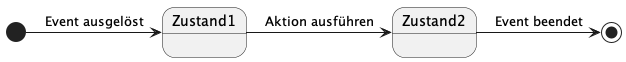
\includegraphics[width=0.95\textwidth]{fig/uml/simple-event.png}
  \caption{Einfaches Event}
  \label{fig:simple-event}
\end{figure}
Während ein Signal ein asynchrones Ereignis ist, ist ein (Call) Event im Allgemeinen synchron. Das bedeutet, dass wenn ein Objekt eine Operation auf einem anderen Objekt aufruft, die Kontrolle vom Sender an den Empfänger übergeben wird, bis die Operation abgeschlossen ist, woraufhin die Kontrolle zum Sender zurückkehrt. 

\item \textbf{Signal}\index{Signal}:
Ein Signal ist ein Ereignis, das von einem Betriebssystem oder einer Anwendung an eine andere Anwendung oder einen Prozess gesendet wird, um eine bestimmte Aktion auszulösen. Signale können zum Beispiel verwendet werden, um einen Prozess zu beenden, ein bestimmtes Verhalten auszulösen oder auf eine bestimmte Situation zu reagieren.
\begin{figure}[!ht]
  \centering
  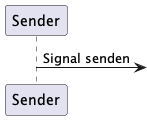
\includegraphics[width=0.25\textwidth]{fig/uml/simple-signal.png}
  \caption{Einfaches Signal}
  \label{fig:simple-signal}
\end{figure}
In der Modellierung der Architektur hat dies eine besondere Bedeutung, da ein Signal ein Objekt repräsentiert, das von einem Objekt asynchron ausgelöst wird und dann von einem anderen empfangen wird. Ein Beispiel hierfür sind Fehlerbehandlungen (Exceptions). Dem Signal ist keine Operation zugeordnet. Die Modellierung einer Klasse oder der Schnittstelle ist ein wichtiger Teil der Spezifikation. So kann definiert werden welches Signal durch die Operationen hinter einem Interface gesendet werden können.

\item \textbf{Nachricht}\index{Nachricht}:
Eine Nachricht ist eine Mitteilung, die von einer Anwendung, einem Prozess oder einem System an eine andere Anwendung, einen Prozess oder ein System gesendet wird. Nachrichten können zum Beispiel verwendet werden, um Daten zwischen verschiedenen Anwendungen oder Systemen auszutauschen, um einen bestimmten Prozess zu starten oder um Informationen über den Status eines Prozesses zu übermitteln. 
\begin{figure}[!ht]
    \centering
    \begin{subfigure}[b]{0.45\textwidth}
      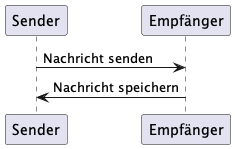
\includegraphics[width=0.8\textwidth]{fig/uml/async-message.png}
      \caption{Asynchrone Nachricht}
      \label{fig:async-msg}
    \end{subfigure}
    \hfill
    \begin{subfigure}[b]{0.45\textwidth}
        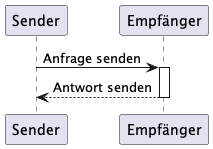
\includegraphics[width=0.75\textwidth]{fig/uml/sync-message.png}
        \caption{Synchrone Nachricht}
        \label{fig:sync-msg}
    \end{subfigure}
    \caption{}
    \label{fig:gesamt}
\end{figure}
\end{itemize}  
Bei Nachrichten gibt es normalerweise einen expliziten Sender und Empfänger, die durch Adressen oder IDs identifiziert werden. Der Sender sendet eine Nachricht an einen bestimmten Empfänger, der die Nachricht empfängt und darauf reagiert.

Dies soll auch nochmals mit den Events verglichen werden. Bei Events hingegen gibt es normalerweise keinen expliziten Sender oder Empfänger. Ein Event tritt auf, und Anwendungen oder Prozesse, die auf dieses Event hören, können darauf reagieren. 
\\\\
Weiter kann das Versenden von Nachrichten sowohl synchron oder asynchron aufgefasst werden. Bei einem synchronen Aufruf existiert eine Sende- und eine Empfangsnachricht. Bei einem asynchronen Aufruf, existiert  typischerweise nur eine Sendenachricht.
\\\\
Signale und Events sind Ereignisse, die in einem System auftreten, während eine Nachricht eine Mitteilung ist, die zwischen verschiedenen Systemen ausgetauscht wird. Signale werden normalerweise zwischen verschiedenen Prozessen oder Anwendungen im selben System verwendet, während Events normalerweise innerhalb einer Anwendung auftreten. Nachrichten werden normalerweise zwischen verschiedenen Anwendungen oder Systemen ausgetauscht.

Events, Signale und Nachrichten bilden die Grundlage für weiterführende Konzepte in der Schnittstellenkonzeptionierung von verteilten Systemen:
\begin{itemize}  
\item \textbf{Remote Procedure Call} (RPC): Hierbei wird eine Funktion auf einem entfernten System aufgerufen, als ob sie lokal ausgeführt würde. Der Aufruf wird über das Netzwerk gesendet und das entfernte System führt die Funktion aus und gibt das Ergebnis zurück.
\item \textbf{Shared Memory}: Hierbei wird ein gemeinsamer Speicherbereich zwischen verschiedenen Knoten im System verwendet, auf den alle Knoten zugreifen können. Dadurch können Daten schnell und effizient zwischen Knoten geteilt werden.
\item \textbf{Datenbank-Replikation}: Hierbei werden Datenbanken auf verschiedenen Knoten im System repliziert, um die Verfügbarkeit und Skalierbarkeit zu verbessern. Änderungen an einer Datenbank werden automatisch an andere replizierte Datenbanken weitergeleitet, um sicherzustellen, dass alle Knoten im System auf dieselben Daten zugreifen können.
\item \textbf{Stream Processing}: Hierbei werden Daten in Echtzeit von verschiedenen Knoten im System gestreamt und verarbeitet, um Echtzeit-Analysen und -Verarbeitung zu ermöglichen. Stream Processing wird oft in Anwendungen wie Finanzdienstleistungen, E-Commerce und Social-Media-Anwendungen eingesetzt.
\end{itemize}  
Diese Möglichkeiten sollen auch mehr im Detail im Kontext der Architekturparadigmen diskutiert werden.

\subsubsection{Kopplung}
Bevor sich den Architekturen zugewendet wird, soll noch einige weitere wichtige Begriffe im Design verteilter Systeme eingebracht werden: Ein wichtiger ist der Kopplungsbegriff. 

Der Kopplungsbegriff ist in verteilten Systemen von entscheidender Bedeutung, da er die Art und Weise beschreibt, wie verschiedene Anwendungen und Systeme in einem verteilten System miteinander interagieren und kommunizieren. Eine falsche Wahl der Kopplungsart kann zu schwerwiegenden Problemen führen, die die Interoperabilität und Integration von Anwendungen in einem verteilten System beeinträchtigen können.
\\\\
Die Wahl der richtigen Kopplungsart kann jedoch auch erhebliche Vorteile bieten. Eine direkte Kopplung kann zu einer höheren Leistung führen und eine bessere Integration von Anwendungen ermöglichen, während eine indirekte Kopplung die Skalierbarkeit und Zuverlässigkeit verbessern kann. Eine losgekoppelte Architektur kann die Flexibilität  und die Ausfallsicherheit erhöhen, während eine strukturelle Kopplung die Zusammenarbeit und Integration von Anwendungen erleichtern kann. Im Detail ist es nochmal in der Tabelle\ref{tab:kopplungsarten} nochmal diskutiert.
\\\\
\begin{table}[!ht]
  \centering
  \caption{Kopplungsarten in verteilten Systemen}
  \label{tab:kopplungsarten}
  \begin{tabular}{|p{4cm}|p{7cm}|}
    \hline
    \textbf{Kopplungsart} & \textbf{Beschreibung} \\ \hline
    Direkte Kopplung & Die Anwendungen und Systeme in einem verteilten System sind direkt miteinander verbunden und kommunizieren direkt miteinander. \\ \hline
    Indirekte Kopplung & Die Anwendungen und Systeme in einem verteilten System kommunizieren über ein gemeinsames Mediator-System oder eine Middleware miteinander. \\ \hline
    Losgekoppelte Kopplung & Die Anwendungen und Systeme in einem verteilten System kommunizieren über Nachrichten, ohne sich direkt zu verbinden. \\ \hline
    Strukturelle Kopplung & Die Anwendungen und Systeme in einem verteilten System sind durch gemeinsame Datenstrukturen oder Datentypen verbunden. \\ \hline
  \end{tabular}
\end{table}
Eine direkte Kopplung tritt auf, wenn Anwendungen oder Systeme direkt miteinander verbunden sind und direkt miteinander kommunizieren. Beispielsweise können zwei Anwendungen über eine Netzwerkverbindung oder einen direkten Datenlink verbunden sein und direkt miteinander kommunizieren.
\\
Eine indirekte Kopplung tritt auf, wenn Anwendungen oder Systeme über ein gemeinsames Mediator-System oder eine Middleware miteinander kommunizieren. Das Mediator-System oder die Middleware stellt eine Abstraktionsschicht bereit, die die Interoperabilität und Integration von Anwendungen in einem verteilten System erleichtert.

Eine losgekoppelte Kopplung tritt auf, wenn Anwendungen oder Systeme über Nachrichten kommunizieren, ohne sich direkt zu verbinden. In diesem Fall sendet eine Anwendung eine Nachricht an eine Middleware oder einen Broker, der die Nachricht an die Empfängeranwendung weiterleitet.

Eine strukturelle Kopplung tritt auf, wenn Anwendungen oder Systeme durch gemeinsame Datenstrukturen oder Datentypen verbunden sind. Beispielsweise können Anwendungen über eine gemeinsame Datenbank oder eine gemeinsame Dateistruktur kommunizieren. Die Tabelle~\ref{tab:kopplungsarten} gibt nochmals einen Überblick mit den Definitionen. 

\subsubsection{Mechanismen und Policies}

Mechanismen\index{Mechanismen} sind die grundlegenden Bausteine oder Funktionen, die zur Implementierung von verteilten Systemen benötigt werden. Policies hingegen sind die Entscheidungsregeln oder Leitlinien, die bestimmen, wie die Mechanismen eingesetzt und betrieben werden.
\\\\
Beispiele von Mechanismen in verteilten Systemen:
\begin{itemize} 
\item Kommunikation: In verteilten Systemen müssen die Knoten miteinander kommunizieren, um Daten auszutauschen und zusammenzuarbeiten. Mechanismen wie Message Passing, Remote Procedure Calls (RPC) und Remote Method Invocation (RMI) ermöglichen diese Kommunikation.
\item Synchronisation: Da verteilte Systeme aus mehreren unabhängigen Knoten bestehen, ist es wichtig, ihre Aktionen und Ressourcenzugriffe zu synchronisieren. Mechanismen wie Locks, Semaphore, Monitore und Barrieren werden verwendet, um die Synchronisation zu erreichen.
\item Replikation: Die Replikation ist ein Mechanismus, bei dem Daten oder Dienste auf mehreren Knoten im verteilten System dupliziert werden, um die Verfügbarkeit, Fehlertoleranz und Leistung zu verbessern.
\item Konsistenz: Um die Datenintegrität in verteilten Systemen aufrechtzuerhalten, müssen Mechanismen zur Gewährleistung der Konsistenz der Daten eingesetzt werden. Beispiele sind sequentielle Konsistenz, kausale Konsistenz, eventual Konsistenz und ACID-Transaktionen.
\end{itemize} 
Beispiele von Policies\index{Policies} in verteilten Systemen:
\begin{itemize} 
\item Ressourcenallokation: In verteilten Systemen müssen Entscheidungen darüber getroffen werden, wie Ressourcen wie Rechenleistung, Speicherplatz und Bandbreite zugewiesen werden. Beispiele für Ressourcenallokations-Policies sind First-Come-First-Served (FCFS), Round Robin, Prioritätswarteschlangen und Fair-Share-Scheduling.
\item Fehlerbehandlung: Policies zur Fehlerbehandlung legen fest, wie verteilte Systeme auf Fehler wie Hardware- oder Softwareausfälle, Netzwerkstörungen oder Datenverlust reagieren. Beispiele für Fehlerbehandlungspolicies sind Retry, Timeout, Fallback auf Alternativen und Datenwiederherstellung.
\item Sicherheit: Sicherheits-Policies bestimmen, wie verteilte Systeme den Schutz von Daten, Diensten und Benutzern gewährleisten. Beispiele sind Authentifizierung, Autorisierung, Verschlüsselung und Auditing.
\item Lastverteilung: Lastverteilungspolicies legen fest, wie die Arbeitslast in verteilten Systemen auf die verschiedenen Knoten verteilt wird, um eine optimale Leistung und Ressourcenauslastung zu erreichen. Beispiele sind statische Lastverteilung, dynamische Lastverteilung und adaptives Load Balancing.
\end{itemize}     

Als Beispiel für die Ausprägung soll die Lastverteilung in einem verteilten System gewählt sein, welche genutzt wird um einen  Webserver-Cluster zu betreiben. In diesem Fall ist Lastverteilung zunächst ein Mechanismus, der die Arbeitslast über mehrere Server oder Knoten verteilt, um eine bessere Leistung, Verfügbarkeit und Skalierbarkeit zu erreichen. Um eine effektive Lastverteilung zu ermöglichen, kann ein Load Balancer eingesetzt werden. Der Load Balancer ist dafür verantwortlich, ankommende Anfragen an die verschiedenen Server im Cluster weiterzuleiten.
Zudem kann die Policy darin bestehen, zu entscheiden, wie die Lastverteilung durchgeführt werden soll. Es gibt verschiedene Policies, die angewendet werden können, wie z. B. Round Robin, Least Connections oder Weighted Round Robin.
\begin{itemize} 
\item Round Robin: Der Load Balancer verteilt die Anfragen gleichmäßig auf alle verfügbaren Server, indem er sie der Reihe nach an jeden Server sendet.
\item Least Connections: Der Load Balancer leitet Anfragen an den Server weiter, der derzeit die wenigsten aktiven Verbindungen hat.
\item Weighted Round Robin: Der Load Balancer verteilt die Anfragen basierend auf dem Gewicht jedes Servers, das normalerweise die Kapazität oder Leistungsfähigkeit des Servers widerspiegelt.
\end{itemize}  
In diesem Beispiel ist der Lastverteilungsmechanismus (Load Balancer) für die Verteilung der Arbeitslast auf die verschiedenen Server im Cluster verantwortlich, während die Lastverteilungspolicy die Methode bestimmt, nach der die Verteilung erfolgen soll (Round Robin, Least Connections oder Weighted Round Robin). Die Policy kann je nach den spezifischen Anforderungen und Zielen des verteilten Systems ausgewählt und angepasst werden, diese Auswahl für jeden Mechanismus anzubieten, kann die Komplexität der Gesamtanwendung aber auch extrem steigern, so das mit einem Mechanismus nicht selten auch direkt die Policy im Mechanismus festgeschrieben wird.  

Ein anderes Beispiel ist näher an der Programmierung. Ein Vergleich zwischen einer API, die die Methoden left, right, up und down verwendet (Variante I), und einer API, die die Methode move(direction) verwendet (Variante II). Variante I ist in der Regel einfacher und direkt, da jede Methode jeweils eine einzelne Bewegungsrichtung repräsentiert. Dies führt zu einer besseren Typsicherheit, da es unwahrscheinlicher ist, dass ungültige Richtungen verwendet werden. Der Nachteil dieser API besteht darin, dass sie aus vier separaten Methoden besteht, was den Code länger und weniger flexibel machen kann. Außerdem ist diese API weniger skalierbar, da für die Hinzufügung neuer Richtungen jeweils neue Methoden erstellt werden müssten.

Auf der anderen Seite erlaubt die API mit der move(direction) Methode mehr Flexibilität, da die gewünschte Richtung als Parameter übergeben wird. Dies erleichtert die Steuerung der Bewegung in verschiedenen Szenarien. Die Skalierbarkeit ist ebenfalls höher, da beim Hinzufügen neuer Richtungen einfach neue Richtungsparameter eingebracht werden können, ohne dass neue Methoden erstellt werden müssen. Da nur eine Methode vorhanden ist, ist der Code kürzer und einfacher zu warten. Der Nachteil dieser API besteht darin, dass sie eine geringere Typsicherheit aufweist, da die Richtung als Parameter übergeben wird und somit die Möglichkeit besteht, dass ungültige oder unerwartete Richtungen verwendet werden.

\subsubsection{Stateful und stateless}
In verteilten Systemen beziehen sich die Begriffe \enquote{stateful}\index{stateful} und \enquote{stateless}\index{stateless} auf die Art und Weise, wie Systemkomponenten den Zustand ihrer Interaktionen verwalten.
\\\\
\textbf{Stateful}:\\
Ein stateful System speichert Informationen über den aktuellen Zustand der Kommunikation zwischen den Komponenten. Das bedeutet, dass ein stateful Service oder eine stateful Anwendung auf vorherige Anfragen oder Interaktionen Bezug nimmt und auf der Grundlage dieser Informationen reagiert. Stateful Systeme sind oft komplexer, da sie den Zustand der Interaktionen aktiv verwalten und speichern müssen. Sie können jedoch auch leistungsfähiger sein, da sie auf der Grundlage früherer Interaktionen individuellere oder optimierte Antworten liefern können.
\\\\
\textbf{Stateless}:\\
Ein stateless System speichert keine Informationen über den aktuellen Zustand der Kommunikation zwischen den Komponenten. Jede Anfrage oder Interaktion wird isoliert betrachtet, ohne Bezug auf frühere Anfragen oder Interaktionen. Stateless Systeme sind in der Regel einfacher zu implementieren und zu skalieren, da sie keine kontinuierliche Zustandsverwaltung erfordern. Sie können jedoch weniger leistungsfähig sein, wenn sie auf Informationen aus früheren Interaktionen angewiesen sind, um effektiv zu funktionieren.
\\\\
In verteilten Systemen können Nachrichtenabhängigkeiten einen Einfluss auf die stateful- oder stateless-Eigenschaften eines Systems haben. Nachrichtenabhängigkeiten treten auf, wenn die Verarbeitung einer Nachricht von der Verarbeitung einer oder mehrerer vorheriger Nachrichten abhängig ist. In solchen Fällen ist es erforderlich, den Zustand der Kommunikation zu verfolgen, um sicherzustellen, dass die Nachrichten in der richtigen Reihenfolge verarbeitet werden und das System korrekt funktioniert.
\begin{itemize}  
\item \textbf{Stateful Systeme}: Nachrichtenabhängigkeiten sind in stateful Systemen von Natur aus einfacher zu handhaben, da diese Systeme bereits den Zustand der Interaktionen verwalten. In stateful Systemen kann die Verarbeitung einer Nachricht auf früheren Nachrichten aufbauen, und das System kann sicherstellen, dass Nachrichten in der richtigen Reihenfolge verarbeitet werden.
\item \textbf{Stateless Systeme}: In stateless Systemen ist die Handhabung von Nachrichtenabhängigkeiten schwieriger, da kein Zustand zwischen den Anfragen gespeichert wird. Um Nachrichtenabhängigkeiten in stateless Systemen zu bewältigen, können Techniken wie das Hinzufügen von Sequenznummern oder Zeitstempeln zu Nachrichten verwendet werden, um die korrekte Reihenfolge der Nachrichtenverarbeitung sicherzustellen. In einigen Fällen müssen stateless Systeme den Zustand extern speichern oder verwalten, um Nachrichtenabhängigkeiten effektiv zu behandeln.
\end{itemize}  

Als ein Beispiel für einen zustandsbehafteten Dienst soll der Dateisystemserver eingebracht werden, welcher auch Zustandsvariant ist.  Ein Dateisystemserver, der seinen Zustand oder seine Zustandsmaschine anpasst, basierend auf den empfangenen Nachrichten, kann daher als zustandsbehaftet oder stateful bezeichnet werden. In einem zustandsbehafteten System speichert der Server Informationen über die Interaktionen mit Clients, wie zum Beispiel offene Dateien, Positionen innerhalb von Dateien oder Benutzerberechtigungen.
\\\\
Wenn der Dateisystemserver eine Anfrage empfängt, z. B. zum Öffnen einer Datei, zum Lesen oder Schreiben von Daten oder zum Ändern von Berechtigungen, aktualisiert er seine Zustandsmaschine entsprechend. Die serverseitige Zustandsmaschine kann Informationen darüber enthalten, welche Dateien gerade geöffnet sind, welche Operationen auf ihnen ausgeführt werden und welche Benutzer Zugriff auf sie haben.

Durch das Beibehalten eines Zustands kann der Dateisystemserver effizienter arbeiten, da er die Informationen über die aktuellen Interaktionen und Operationen speichert und darauf zugreifen kann, ohne sie jedes Mal neu abrufen oder berechnen zu müssen. Allerdings bringt diese zustandsbehaftete Architektur auch Herausforderungen in Bezug auf Skalierbarkeit, Fehlertoleranz und Ressourcenverwaltung mit sich.

Die Wahl zwischen stateful und stateless Architekturen von den Anforderungen des verteilten Systems ab. Stateless Systeme bieten Vorteile in Bezug auf Einfachheit und Skalierbarkeit, während stateful Systeme besser für Anwendungen geeignet sind, bei denen der Kontext früherer Interaktionen für die korrekte Bearbeitung notwendig sind. 

\subsubsection{Transaktion}
In verteilten Systemen ist eine Transaktion eine Sequenz von Operationen, die auf verteilten Ressourcen oder Daten ausgeführt werden, um eine bestimmte Aufgabe oder Funktion zu erfüllen. Transaktionen sind wichtig, um die Konsistenz und Integrität von Daten in verteilten Systemen zu gewährleisten, insbesondere bei gleichzeitigen Zugriffen und Änderungen durch verschiedene Benutzer oder Prozesse.

Transaktionen in verteilten Systemen sollten die ACID-Eigenschaften (Atomicity, Consistency, Isolation, Durability) erfüllen:
\begin{itemize}
\item Atomicity (Atomarität): Eine Transaktion besteht aus einer Reihe von Operationen. Entweder werden alle Operationen erfolgreich ausgeführt und die Transaktion ist abgeschlossen, oder bei einem Fehler werden alle Operationen rückgängig gemacht, als ob die Transaktion nie stattgefunden hätte.
\item Consistency (Konsistenz): Transaktionen stellen sicher, dass das verteilte System von einem konsistenten Zustand in einen anderen konsistenten Zustand übergeht, auch wenn Fehler oder gleichzeitige Zugriffe auftreten.
\item Isolation (Isolierung): Jede Transaktion wird so ausgeführt, als ob sie isoliert von anderen gleichzeitig laufenden Transaktionen wäre. Dies bedeutet, dass die Zwischenergebnisse einer Transaktion für andere Transaktionen nicht sichtbar sind, bis die Transaktion abgeschlossen ist.
\item Durability (Dauerhaftigkeit): Sobald eine Transaktion abgeschlossen ist, sind ihre Änderungen dauerhaft im System gespeichert, selbst im Falle von Systemausfällen oder Fehlern.
\end{itemize}
Beispiele für Transaktionen in verteilten Systemen:
\begin{itemize}
\item Bankwesen: In einem verteilten Banksystem können Transaktionen verwendet werden, um Geldtransfers zwischen Konten durchzuführen. Die Transaktion stellt sicher, dass das Geld vom Senderkonto abgezogen und dem Empfängerkonto hinzugefügt wird, wobei die Konsistenz der Kontostände gewährleistet ist.
\item E-Commerce: In einem verteilten E-Commerce-System können Transaktionen verwendet werden, um Bestellungen und Zahlungen zu verarbeiten. Die Transaktion kann die Aktualisierung des Lagerbestands, die Berechnung von Steuern und Versandkosten, die Reservierung von Artikeln und die Verarbeitung der Zahlung beinhalten.
\item Verteilte Datenbanken: Bei verteilten Datenbanken werden Transaktionen verwendet, um sicherzustellen, dass mehrere Operationen, wie das Hinzufügen, Aktualisieren oder Löschen von Datensätzen, konsistent und gleichzeitig durchgeführt werden, ohne dass Inkonsistenzen oder Datenverluste auftreten.
\end{itemize}
Allerdings erfordert die Implementierung von Transaktionen in verteilten Systemen auch zusätzliche Überlegungen hinsichtlich Leistung, Fehlertoleranz und Koordination zwischen den beteiligten Knoten.
\\\\
Verschachtelte Transaktionen sind eine Erweiterung des grundlegenden Transaktionskonzepts, bei dem Transaktionen innerhalb einer übergeordneten Transaktion ausgeführt werden können. Diese innere Transaktion wird als \enquote{Untertransaktion} oder \enquote{Nested Transaction} bezeichnet. Eine verschachtelte Transaktion erlaubt es, dass Untertransaktionen unabhängig voneinander abgeschlossen oder abgebrochen werden, ohne die übergeordnete Transaktion als Ganzes zu beeinflussen.

Verschachtelte Transaktionen bieten Vorteile in Bezug auf Modularität, Fehlerbehandlung und Leistung, insbesondere in verteilten Systemen und bei komplexen Abläufen. Sie ermöglichen es, Teile einer größeren Transaktion separat abzuschließen und bei Fehlern nur die betroffenen Teile zurückzurollen, anstatt die gesamte Transaktion rückgängig zu machen.
\\\\
Ein Transaktionsmanager, auch als Transaktionskoordinator oder Transaktionsmonitor bezeichnet, ist eine Komponente in einem verteilten System, die für das Management und die Koordination von Transaktionen verantwortlich ist. Der Transaktionsmanager hat folgende Hauptaufgaben:
\begin{itemize}
\item Koordination: Der Transaktionsmanager koordiniert die beteiligten Ressourcen und Knoten in einer verteilten Transaktion, um sicherzustellen, dass sie konsistent und korrekt ausgeführt wird.
\item Protokollierung und Wiederherstellung: Der Transaktionsmanager führt ein Transaktionsprotokoll, um Änderungen und Aktivitäten während der Transaktion aufzuzeichnen. Im Falle eines Fehlers oder Systemausfalls verwendet der Transaktionsmanager das Protokoll, um den Zustand der beteiligten Ressourcen wiederherzustellen und die Transaktion entweder abzuschließen oder zurückzurollen.
\item Isolierung und Synchronisation: Der Transaktionsmanager stellt sicher, dass Transaktionen isoliert voneinander ausgeführt werden, um die Konsistenz und Integrität der Daten zu gewährleisten. Er ist auch für die Synchronisation von Zugriffen und Aktualisierungen auf verteilte Ressourcen verantwortlich, um Deadlocks und Konflikte zu vermeiden.
\item Commit und Rollback: Der Transaktionsmanager ist verantwortlich für das endgültige Commit (Abschluss) oder Rollback (Rückgängigmachung) einer Transaktion. Bei erfolgreicher Ausführung aller Operationen wird die Transaktion abgeschlossen und die Änderungen dauerhaft gespeichert. Im Falle eines Fehlers oder einer nicht erfüllten Bedingung führt der Transaktionsmanager ein Rollback durch, um die betroffenen Ressourcen in ihren vorherigen Zustand zurückzusetzen.
\end{itemize}
Ein Transaktionsmanager spielt eine entscheidende Rolle bei der Sicherstellung der Konsistenz, Integrität und Fehlertoleranz in verteilten Systemen, die Transaktionen verwenden. Das Konzept ist auch größer als aus einfachen Beispielen hervorgeht, die Bedeutung wird erst in der Flexibilität  deutlich. Dennoch soll ein Beispiel versucht werden, wo drei unabhängige Dienste: Flug, Hotel und Mietwagen zu einem neuen, vorher nicht vorhandenen Dienst zusammengefügt wird. 

Zuerst beginnt der Transaktionsmanager eine neue Transaktion. In dieser Transaktion werden die erforderlichen Ressourcen von den drei Diensten reserviert: Flugbuchung, Hotelbuchung und Mietwagenbuchung. Anschließend prüft der Transaktionsmanager, ob alle erforderlichen Ressourcen erfolgreich reserviert wurden und ob die Verfügbarkeit für den gewünschten Zeitraum gegeben ist.

Wenn alle Reservierungen erfolgreich sind und die Verfügbarkeit für den gewünschten Zeitraum bestätigt wurde, führt der Transaktionsmanager die Transaktion aus und erstellt die Urlaubsreise. Dabei wird der Gesamtpreis für Flug, Hotel und Mietwagen berechnet und dem Kunden in Rechnung gestellt. Nach erfolgreicher Zahlung bestätigt der Transaktionsmanager die Buchungen für die einzelnen Dienste und speichert die Informationen für die Urlaubsreise im System.

Falls jedoch eine oder mehrere Reservierungen nicht erfolgreich sind oder die Verfügbarkeit für den gewünschten Zeitraum nicht gegeben ist, wird der Transaktionsmanager die Transaktion abbrechen. In diesem Fall werden alle bisher reservierten Ressourcen für Flug, Hotel und Mietwagen freigegeben und der Kunde wird darüber informiert, dass die Urlaubsreise nicht erstellt werden konnte.

Der Transaktionsmanager stellt sicher, dass entweder alle Dienste erfolgreich kombiniert und die Urlaubsreise erstellt wird, oder keine der Reservierungen erfolgt und die Ressourcen wieder freigegeben werden. Dadurch wird ein konsistenter Zustand in den verteilten Systemen gewährleistet und es wird verhindert, dass teilweise reservierte oder unvollständige Urlaubsreisen entstehen.
\subsubsection{Message Passing}
Message Passing ist ein Kommunikationsparadigma in verteilten Systemen, bei dem Prozesse oder Komponenten Nachrichten austauschen, um Daten zu übertragen oder Aufgaben zu koordinieren. Es ist ein grundlegendes Konzept in der Kommunikation zwischen verteilten Einheiten und bildet die Basis für viele verteilte Systemarchitekturen, aber auch darüber hinaus.
Message Passing ist ein Konzept für die Nebenläufigkeits-Programmierung (Concurrent programming), der parallelen Programmierung (Parallel programming), der objektorientierten Programmierung und der Interprozesskommunikation.

Im Message Passing werden Nachrichten, die Daten oder Anweisungen enthalten, zwischen Prozessen oder Komponenten übermittelt. Die Kommunikation erfolgt in der Regel asynchron, d. h., der sendende Prozess wartet nicht darauf, dass der empfangende Prozess die Nachricht empfängt oder verarbeitet. Dies ermöglicht eine lose Kopplung der Komponenten und erleichtert die Skalierung und Fehlertoleranz des Systems. Die Eigenschaften von Message Passing können wie folgt zusammengefasst werden:
\begin{itemize}
\item Asynchrone Kommunikation: Die Kommunikation ist in der Regel asynchron, wodurch Prozesse unabhängig voneinander weiterarbeiten können, ohne auf Antworten warten zu müssen.
\item Lose Kopplung: Die Kommunikation zwischen Prozessen ist indirekt und erfordert keine direkte Kenntnis der beteiligten Prozesse, was zu einer losen Kopplung der Komponenten führt.
\item Skalierbarkeit: Message Passing eignet sich gut für verteilte Systeme mit einer großen Anzahl von Prozessen oder Komponenten, da es einfacher ist, zusätzliche Knoten hinzuzufügen und die Kommunikation zwischen ihnen zu verwalten.
\end{itemize}
Beispiele für Message Passing in verteilten Systemen:
\begin{itemize}
\item Message Queues: Message Queues sind Datenstrukturen, die zum Speichern und Übertragen von Nachrichten zwischen verteilten Prozessen verwendet werden. Beispiele für Message Queue-Systeme sind RabbitMQ, Apache Kafka und Amazon SQS. Sie ermöglichen die asynchrone Kommunikation und die Entkopplung von sendenden und empfangenden Prozessen.

\item Message Passing Interface (MPI): MPI ist ein Standard für die Kommunikation zwischen Prozessen in verteilten Systemen, insbesondere in High-Performance-Computing-Umgebungen. MPI stellt Funktionen zum Senden und Empfangen von Nachrichten, Synchronisation von Prozessen und Gruppenkommunikation bereit.

\item Publish-Subscribe-Systeme: In diesem Modell senden Publisher Nachrichten an Topics, während Subscriber Nachrichten von den Topics empfangen, die sie abonniert haben. Beispiele für Publish-Subscribe-Systeme sind Google Cloud Pub/Sub, Apache Pulsar und MQTT. Dieses Modell ist ereignisgetrieben und ermöglicht eine lose Kopplung der beteiligten Prozesse.
\end{itemize}
Message Passing ist ein grundlegendes Konzept in verteilten Systemen und ermöglicht die Kommunikation und Koordination zwischen Prozessen oder Komponenten in einer skalierbaren und fehlertoleranten Weise.

Das Actor-Modell ist ein Konzept für das Design von verteilten Systemen, das auf der Idee von unabhängigen Entitäten basiert, die als \enquote{Actoren} bezeichnet werden. Actoren sind grundlegende Recheneinheiten, die einen Zustand besitzen und in der Lage sind, Nachrichten zu empfangen und zu verarbeiten. Es setzt auf das Konzept von Message Passing auf. In diesem Modell kommunizieren Actoren ausschließlich über asynchrone Nachrichtenübermittlung, wodurch sie lose gekoppelt und hochgradig parallelisierbar sind. Die Hauptprinzipien des Actor-Modells sind:
\begin{itemize}
\item Isolation: Jeder Actor verwaltet seinen eigenen Zustand und verarbeitet Nachrichten unabhängig von anderen Actoren. Diese Isolation ermöglicht eine hohe Fehlertoleranz und erleichtert die Wartung und Skalierung des Systems.

\item Nachrichtenbasierte Kommunikation: Actoren kommunizieren über asynchrone Nachrichten. Nachrichten werden in Mailboxen abgelegt und von Actoren verarbeitet, wenn sie dazu bereit sind. Dieser Ansatz reduziert die Notwendigkeit von Locking- und Synchronisierungsmechanismen und ermöglicht eine hohe Parallelität.

\item Lokalitätstransparenz: Actoren können unabhängig von ihrer physischen Lage im verteilten System agieren. Die Kommunikation zwischen Actoren ist transparent und unabhängig von der Verteilung der Actoren im System.

\item Fehlertoleranz: Durch die Isolation der Actoren und ihre unabhängige Verarbeitung von Nachrichten können Fehler auf einzelne Actoren beschränkt bleiben, ohne das gesamte System zu beeinträchtigen. Das Actor-Modell unterstützt auch Supervision, bei der ein Actor die Verantwortung für das Überwachen und Wiederherstellen anderer Actoren bei Fehlern übernimmt.
\end{itemize}


\subsubsection{Idempotent}

Idempotenz\index{idempotenz} ist ein wichtiger Begriff in der Informatik und bezieht sich auf die Eigenschaft von Operationen, die wiederholt ausgeführt werden können, ohne dass sich das Ergebnis nach der ersten Anwendung ändert. Eine idempotente Operation ist eine, bei der das mehrmalige Anwenden auf dasselbe Eingabematerial das gleiche Ergebnis liefert, als ob sie nur einmal ausgeführt worden wäre.

Die Bedeutung von Idempotenz für verteilte Systeme liegt in ihrer Fähigkeit, die Robustheit und Zuverlässigkeit zu verbessern, insbesondere in Situationen, in denen Netzwerkfehler, Duplizierung von Nachrichten oder unvorhersehbare Verzögerungen auftreten können. In verteilten Systemen kann es schwierig sein, den genauen Zustand des Systems zu bestimmen, und es kann nicht garantiert werden, dass Nachrichten oder Anforderungen immer in der richtigen Reihenfolge oder genau einmal ankommen.

Indem idempotente Operationen in verteilten Systemen verwendet werden, können einige der Herausforderungen im Zusammenhang mit Fehlern und Unvorhersehbarkeiten bewältigt werden:
\begin{itemize}
\item Wiederholung von Anfragen: Wenn ein Client in einem verteilten System keine Antwort von einem Server erhält, kann es schwierig sein, festzustellen, ob die Anfrage verloren gegangen ist oder ob der Server die Anfrage einfach noch nicht verarbeitet hat. In solchen Fällen kann die Wiederholung einer idempotenten Anfrage ohne negative Auswirkungen erfolgen, da mehrmaliges Senden derselben Anfrage dasselbe Ergebnis wie das einmalige Senden liefert.
\item Fehlertoleranz: Idempotente Operationen können dazu beitragen, die Fehlertoleranz von verteilten Systemen zu erhöhen, indem sie die Auswirkungen von Nachrichtenduplikationen oder Netzwerkfehlern minimieren. Da idempotente Operationen dieselben Ergebnisse liefern, unabhängig davon, wie oft sie angewendet werden, können sie dazu beitragen, den Systemzustand trotz solcher Fehler konsistent zu halten.
\item Vereinfachung der Systementwicklung: Idempotenz kann dazu beitragen, die Komplexität von verteilten Systemen zu verringern, indem sie die Notwendigkeit von komplizierten Mechanismen zur Handhabung von Zustandsänderungen oder Fehlerbehebungen verringert. Da idempotente Operationen immer dieselben Ergebnisse liefern, unabhängig von ihrer Anwendungsreihenfolge, können Entwickler weniger Zeit damit verbringen, solche Mechanismen zu entwickeln, und sich stattdessen auf die Implementierung der Kernfunktionalität des Systems konzentrieren.
\end{itemize}

Ein Beispiel für die Verwendung von Idempotenz in verteilten Systemen ist das PUT-HTTP-Verb in HTTP-APIs. Das PUT-Verb wird verwendet, um eine Ressource mit einer bestimmten ID zu aktualisieren oder zu ersetzen. Wenn eine PUT-Anfrage mehrmals gesendet wird, bleibt das Ergebnis gleich, als ob die Anfrage nur einmal gesendet wurde. 


\subsubsection{Distributed Hash Table, DHT}

Distributed Hash Tables (DHTs\index{DHT}) sind ein Schlüssel-Wert-Speichersystem, das in verteilten Systemen eingesetzt wird. Sie bieten eine effiziente und dezentrale Möglichkeit, Schlüssel-Wert-Paare in einem Peer-to-Peer-Netzwerk zu speichern und abzurufen. In DHTs sind die Knoten des Netzwerks gleichberechtigt und es gibt keine zentrale Instanz, die die Speicherung und den Zugriff auf die Daten kontrolliert.

Die mathematische Grundlage von DHTs ist der konsistente Hashing-Algorithmus, der wie folgt dargestellt werden kann:

\begin{itemize}
\item Gegeben sei ein Schlüsselraum von $0$ bis $2^m - 1$, wobei $m$ die Anzahl der Bits ist, die zur Darstellung der Schlüssel verwendet werden.
\item Jeder Knoten und jeder Schlüssel im DHT wird durch eine eindeutige ID im Schlüsselraum repräsentiert. Die IDs können durch Hash-Funktionen wie z.B. SHA-1 erzeugt werden.
\item Die Knoten sind in einem logischen Ring angeordnet, basierend auf ihren IDs, der als \enquote{Ringraum} bezeichnet wird. Die Position eines Knotens im Ringraum wird durch seine ID bestimmt.
\item Um einen Wert für einen bestimmten Schlüssel zu speichern oder abzurufen, wird der Schlüssel zunächst durch dieselbe Hash-Funktion gehasht, die für die Erzeugung der Knoten-IDs verwendet wurde.
\item Der gehashte Schlüssel wird dann im Ringraum lokalisiert, und der zuständige Knoten für diesen Schlüssel ist derjenige, dessen ID gleich oder unmittelbar nach der gehashten Schlüssel-ID liegt. Dieser Knoten wird als \enquote{Verantwortlicher} für den Schlüssel bezeichnet.
\item Jeder Knoten speichert Informationen über eine kleine Anzahl anderer Knoten im Netzwerk, die als \enquote{Nachbarn} bezeichnet werden. Diese Nachbarn dienen zur Weiterleitung von Anfragen für Schlüssel, für die der aktuelle Knoten nicht verantwortlich ist.
\item Bei Änderungen im Netzwerk, wie zum Beispiel beim Hinzufügen oder Entfernen von Knoten, werden die Schlüssel-Wert-Paare entsprechend neu verteilt, um die Belastung gleichmäßig auf alle Knoten im Netzwerk zu verteilen.
\end{itemize}


\label{Woche03}\subsection{Architekturparadigmen}

In den Verteilten Systemen gibt es verschiedene Architekturparadigmen, die beschreiben, wie Software- oder Computersysteme strukturiert und organisiert werden können. Zunächst soll ein Überblick gegeben werden, bevor die Ansätze genauer diskutiert werden. Die wichtigsten Architekturparadigmen für diese Ausarbeitung sind:
\begin{itemize}  
\item \textbf{Schichtenarchitektur} (Layered Architecture): Hierbei wird das System in mehrere Schichten unterteilt, wobei jede Schicht eine bestimmte Funktion erfüllt und auf der darunter liegenden Schicht aufbaut. Ein Beispiel ist die dreischichtige Architektur, die aus einer Präsentationsschicht, einer Anwendungsschicht und einer Datenspeicherschicht besteht.

\item \textbf{Client-Server-Architektur}: Hierbei wird das System in einen Client und einen Server unterteilt, wobei der Client Anfragen an den Server sendet und dieser daraufhin Antworten liefert. Diese Architektur eignet sich gut für Anwendungen, bei denen der Client nur eine begrenzte Anzahl von Funktionen benötigt, während der Server die komplexen Berechnungen durchführt.

\item \textbf{Service-Orientierte Architektur} (SOA): Hierbei wird das System in Services unterteilt, die unabhängig voneinander entwickelt und bereitgestellt werden können. Diese Architektur ermöglicht die flexible Integration von Services, um komplexe Anwendungen zu erstellen.

\item \textbf{Ereignisgesteuerte Architektur} (Event-Driven Architecture): Hierbei reagiert das System auf Ereignisse, indem es entsprechende Aktionen ausführt. Diese Architektur wird oft in Systemen verwendet, die auf (beinah) Echtzeitereignisse reagieren müssen, wie z.B. in der Finanzindustrie oder in der Telekommunikation.

\item \textbf{Microservices-Architektur}: Hierbei wird das System in kleine, unabhängige Services unterteilt, die jeweils eine spezifische Funktion erfüllen. Diese Architektur ermöglicht eine bessere Skalierbarkeit und Flexibilität, da jeder Service unabhängig voneinander entwickelt, getestet und bereitgestellt werden kann.

\item \textbf{Peer-to-Peer-Architektur} (P2P): Hierbei wird das System in ein Netzwerk von gleichwertigen Teilnehmern unterteilt, die direkt miteinander kommunizieren können, ohne auf einen zentralen Server angewiesen zu sein. Diese Architektur wird oft in Filesharing- und Kryptowährungsanwendungen verwendet.
\end{itemize}  
Um Architekturmuster zu verstehen ist es auch wichtig zu hinterfragen, wie die Komponenten und Recheneinheiten in einem System angeordnet sind. Um diese zu benennen wird häufig der Begriff \enquote{node}~\cite{tanenbaum2017distributed}~(Knoten) eingeführt. \textbf{Unter einer node versteht man ein autonomes Computerelement}, sei es Hardware-Systeme oder Software-Prozesse. 
Es gibt noch weitere Architekturparadigmen, aber diese sechs sind die in diesem Skript wichtigsten und am häufigsten verwendeten. Bei allen Architekturen darf man die historische Komponente nicht vergessen. Die meisten Architekturen lassen sich daher auch aus dem Grundtypos einer Schichtenarchitektur erklären. 

\subsubsection{Schichtenarchitektur}

Schichtenmodelle spielen eine wichtige Rolle bei der Architektur von verteilten Systemen, indem sie hierarchische Strukturen definieren, die bestimmte Funktionen und Dienste je Schicht kapseln.
\\\\
Das Schichtenmodell ist ein durchdachtes Konzept, das auf dem Prinzip von \enquote{Teile und Herrsche} basiert und ein System in mehrere Ebenen unterteilt. Die Bedeutung von Schichtenmodelle für die Architektur von verteilten Systemen besteht darin, dass sie es ermöglichen, komplexe Systeme in kleinere, einfachere Teile zu zerlegen, die unabhängig voneinander entwickelt, getestet und gewartet werden können. Jede Schicht kann als eine separate Komponente oder ein separates Subsystem implementiert werden, das von anderen Schichten isoliert ist und über definierte Schnittstellen kommunizieren kann. Die besondere Bedeutung der Schnittstellen kann für den langfristen Erfolg nicht stark genug herausgestellt werden.

Durch die Verwendung von Schichtenmodellen wird auch die Interoperabilität zwischen verschiedenen Systemen erleichtert. Unabhängigen Systemen erlaubt es einen Datenaustausch. Da jeder Hersteller oder Entwickler eine bestimmte Schicht des Modells implementieren und somit sicherstellen kann, ist die Bindung alleine über die Schnittstellen der Schichten zu schaffen. So ist das System im besten Falle mit anderen Systemen über die definierten Schnittstellen immer kompatibel.

Ein weiterer Vorteil bei der Verwendung der Architektur besteht darin, dass sie die Wiederverwendbarkeit von Komponenten und Diensten erleichtert. Da jede Schicht bestimmte Funktionen und Dienste bereitstellt, können sie in verschiedenen Systemen und Anwendungen wiederverwendet werden, ohne dass eine Neuentwicklung erforderlich ist. Schichten können auch dazu beitragen, die Sicherheit von Anwendungen zu verbessern. Durch die Trennung von Funktionen und Verantwortlichkeiten kann die Sicherheit jeder Schicht verbessert werden, ohne dass die Sicherheit des gesamten Systems beeinträchtigt wird. So kann beispielsweise eine Schicht, die für die Authentifizierung und Autorisierung von Benutzern verantwortlich ist, unabhängig von anderen implementiert und gewartet werden, um eine höhere Sicherheit zu gewährleisten.

Die Idee der Schichtenmodelle für verteilte Systeme geht auf die 1970er Jahre zurück, als verschiedene Organisationen begannen, Netzwerkprotokolle zu standardisieren und zu entwickeln. Das erste bekannte Schichtenmodell für Netzwerkprotokolle war das \enquote{Department of Defense (DoD) Internet Model}, das 1982 von der US-amerikanischen Regierung eingeführt wurde. Dieses Modell hatte vier Schichten: Anwendung, Transport, Internet und Netzwerkzugang.

In den 1980er Jahren wurde das Open Systems Interconnection (OSI)-Referenz-modell von der Internationalen Organisation für Normung (ISO) eingeführt. Es war ein sehr generisches Schichtenmodell für Netzwerkprotokolle und hatte sieben Schichten: Anwendung, Darstellung, Sitzung, Transport, Netzwerk, Data Link und Physikalisch. Das OSI-Modell hatte den Vorteil, dass es herstellerunabhängig war und Interoperabilität zwischen verschiedenen Netzwerkprotokollen als definiertes Ziel umsetzte.

Auch andere Organisationen begannen ihre eigenen Schichtenmodelle für Netzwerkprotokolle zu entwickeln. Zum Beispiel verwendete die Digital Equipment Corporation (DEC) ein Schichtenmodell mit fünf Schichten, das DECnet genannt wurde. IBM entwickelte auch ein eigenes, das Systems Network Architecture (SNA) hieß.

In den 1990er Jahren gewannen TCP/IP-basierte Netzwerkprotokolle zunehmend an Bedeutung und das OSI-Referenzmodell wurde weniger populär. TCP/IP hatte auch ein Schichtenmodell, welches dem DoD Modell sehr ähnlich war. 
\\\\
In den letzten Jahren haben Schichtenmodelle auch bei der Entwicklung von verteilten Systemen jenseits von Netzwerken an Bedeutung gewonnen. Auch wenn das Modell manchmal recht angestaubt erscheint, wird es zum Beispiel verwendet, um die Architektur von Cloud-basierten Anwendungen oder Microservices zu beschreiben.
\\\\
Um die Kraft eines Schichtenmodells zu verdeutlichen, soll auch nochmal diskutiert werden, nach welchen Ansätzen ein System in Schichten unterschieden werden kann. Doch hierzu soll weniger der deutsche Begriff Schicht genutzt sein, sondern vielmehr  die englischen Begriffe \enquote{Tier} (Ebene) und \enquote{Layer} (Schicht). Diese Begriffe sind in dem Kontext gut etabliert und besser geeignet, um die notwendige Diskussion zu führen:
\\\\
Ein (Software-)\enquote{Layer} beschreibt eine logische Gruppierung von Funktionen innerhalb einer Anwendung oder eines Systems. Layer werden in der Regel vertikal angeordnet und können aus mehreren Tiers bestehen, die gemeinsam eine Schicht bilden. Jedes Layer erfüllt eine spezifische Funktion und  kommuniziert über definierte Schnittstellen mit der darüber oder darunter liegenden Schicht. Beispiele für Layer in verteilten Systemen sind die Three-Layer Architekturen, die in Anwendungslogik-Schicht, die Datenzugriffs-Schicht oder die Präsentations-Schicht unterteilt sind.
\begin{figure}[!h]
  \centering
  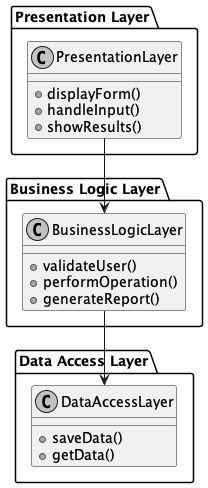
\includegraphics[width=0.25 \textwidth]{fig/uml/simple-layers.png}
  \caption{Einfaches Schichtenmodell}
  \label{fig:simple-layer}
\end{figure}

In der Graphik \ref{fig:simple-layer} sind drei Layer beschrieben, die jeweils eine Schicht darstellen:
\begin{itemize}
\item Das \enquote{Presentation Layer} enthält die Klasse \enquote{PresentationLayer}, die für die Benutzeroberfläche und die Interaktion mit dem Benutzer zuständig ist.

\item Das \enquote{Business Logic Layer} enthält die Klasse \enquote{BusinessLogicLayer}, die die Geschäftslogik und die Regeln enthält, die die Anwendung ausführen.

\item Das \enquote{Data Access Layer} enthält die Klasse \enquote{DataAccessLayer}, die für den Zugriff auf Datenbanken oder andere Datenquellen zuständig ist.
\end{itemize}
Die Pfeile zwischen den Komponenten zeigen die Abhängigkeiten zwischen den Schichten an. Die Presentation Layer ist von der Business Logic Layer abhängig und die Business Logic von der Data Access.
\\\\
Ein \enquote{Tier} hingegen beschreibt die physische oder logische Aufteilung von Anwendungen oder Systemen auf verschiedene Server oder Endgeräte. Jedes Tier hat normalerweise eine spezifische Funktion, wie z.B. Datenbank-Tier, Anwendungs-Tier oder Präsentations-Tier. Die Tiers sind normalerweise durch eine Netzwerkverbindung miteinander verbunden, und jede Schicht kommuniziert direkt mit jeder benachbarten Schicht.
\begin{figure}[!h]
  \centering
  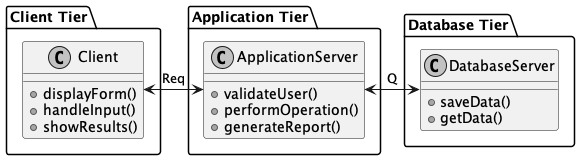
\includegraphics[width=0.80\textwidth]{fig/uml/simple-tiers.png}
  \caption{Einfaches Tier Modell}
  \label{fig:simple-tier}
\end{figure}
In diesem Beispiel eines Three-Tier-Models existieren drei Komponenten, die jeweils ein Tier darstellen:
\begin{itemize}
\item Das \enquote{Client Tier} enthält die Klasse \enquote{Client}, die für die Benutzeroberfläche und die Interaktion mit dem Benutzer auf dem Client-Gerät zuständig ist.

\item Das \enquote{Application Tier} enthält die Klasse \enquote{ApplicationServer}, die die Geschäftslogik und die Regeln enthält, die die Anwendung auf dem Application Server ausführen.

\item Das \enquote{Database Tier} enthält die Klasse \enquote{DatabaseServer}, die für den Zugriff auf Datenbanken oder andere Datenquellen auf dem Database Server zuständig ist.
\end{itemize}
Die Pfeile zwischen den Komponenten zeigen die Kommunikation zwischen den Tiers an. Der Client sendet eine Anfrage an den Application Server und der Application Server leitet die Anfrage an den Database Server weiter. Der Database Server gibt dann eine Antwort zurück, die über den Application Server an den Client zurückgesendet wird.
\\\\
Im Zweifel können Tiers und Layers die gleichen Namen besitzen, obwohl sich Ihre Motivation im Design unterscheidet. Vielleicht hilft auch nochmal die Sicht auf die Ziele der unterschiedlichen Zuschnitte. Im Layer-Modell sind folgende Ziele eher mit dem gewünschten Zuschnitt verbunden:
\begin{itemize}
\item Bestimmung der Funktionen und die Zuordnung zu logischen Komponenten mit fester Verantwortung und festen Schnittstellen. 
\item Bessere Wartbarkeit und die Flexibilität bei der Ausgestaltung. Komponenten können ausgetauscht und ersetzt werden, da sie festen Schnittstellendefinitionen genügen.  
\end{itemize}
Der Fokus auf die Tiers adressiert mehr die Anforderung an die physischen/logische Architektur des verteilten Systems, diese sollen hier kurz nochmal erwähnt sein:
\begin{itemize}
\item Bestimmung der möglichen Skalierung auf (logische/virtuelle) Hardware und die generelle Zuweisung der logischen Komponenten.
\item Bestimmung der (Netzwerk-)Charakteristiken für die Kommunikation zwischen den Komponenten.
\end{itemize}
Ein besonderer Architekturtyp ist eine \enquote{Single-Node-Application}, welche in einem Verteilten System als 1-Tier-Architektur verstanden werden kann.

\subsubsection{Single Node}

Eine Single-Node-Application ist ein Architekturtyp welche das Ziel hat, die Anwendung auf einem einzelnen Knoten in einem verteilten System auszuführen. Im Gegensatz zu einer Anwendung, die auf mehreren Knoten ausgeführt wird, braucht es hier keine Verteilung der Funktionen oder Daten über den logischen/physikalischen Knoten hinaus. Der Knoten kann ein physischer Server oder eine virtuelle Maschine sein.
\\\\
Ein Beispiel für eine Single-Node-Application in einem verteilten System könnte eine Anwendung sein, die Daten von verschiedenen Systemen sammelt und verarbeitet. Obwohl die Anwendung nur auf einem Knoten ausgeführt wird, muss sie möglicherweise mit verschiedenen Systemen und Datenquellen kommunizieren, dies ist in der Architektur, nicht nur, nicht ausgeschlossen, sondern eine erwünschte Eigenschaft.
\\\\
Obwohl Single-Node-Applications nicht auf mehreren Knoten verteilt sind, können sie immer noch von den Vorteilen einer Verteilung profitieren, wie z.B. Skalierbarkeit, Zuverlässigkeit und Flexibilität. Weiter können
Single-Node-Applications von Middleware-Technologien wie Message Queues und RPC profitieren, die die Interoperabilität zwischen verschiedenen Anwendungen und Systemen erleichtern. Eine Einschränkung ist, das die Middleware nicht primär für die kooperative Arbeit genutzt wird, sondern für das Sammeln und Aufbereiten der Daten. Diese Überlegungen münden in die Bestrebung der Formulierung eines Best Practice Entwurfmusters (Pattern) des sogenannten Single-Node-Pattern miteinfließen. Das Pattern hat seinen Nutzen bereits in verschiedenen Szenarien aufgezeigt, wie zum Beispiel:
\begin{itemize}
\item Entwicklung und Testen: Das Pattern kann verwendet werden, um Anwendungen auf einem einzigen Knoten während der Entwicklung und Tests auszuführen, um Zeit und Ressourcen zu sparen, die für die Bereitstellung und Verwaltung von verteilten Systemen erforderlich sind.
\item Kleine Anwendungen: Das Single-Node-Pattern kann nützlich sein, wenn die Anwendung klein ist und nicht viele Ressourcen benötigt. In diesem Fall kann eine entsprechende Implementierung ausreichend sein, um die Anforderungen der Anwendung zu erfüllen.
\item Datenintensive Anwendungen: Das Single-Node-Pattern ist auch für datenintensive Anwendungen nützlich, bei denen die Daten auf einem einzigen Knoten gespeichert und verarbeitet werden können.
\end{itemize}
Das Single-Node-Pattern kann mit verschiedenen Technologien implementiert werden, wie z.B. Container-Technologien (Docker), virtuelle Maschinen (VMs) oder Serverless-Computing (AWS Lambda). Die Wahl der Technologie hängt von den Anforderungen der Anwendung und den verfügbaren Ressourcen ab, welche Vor- und Nachteile verbunden sind, soll im Kapitel über die \enquote{Realisierung} miteinander diskutiert werden. 

\textbf{Das Single-Node-Pattern bezieht sich auf die Verwendung eines einzigen Serverknotens oder einer einzelnen Instanz des zu erbringenden Dienstes, anstatt mehrere Knoten zu verwenden, um denselben Dienst bereitzustellen}. Hier sind einige Beispiele von Unternehmen, die dieses Muster einsetzen:
\begin{itemize}
\item Netflix\footnote{https://medium.com/@narengowda/netflix-system-design-dbec30fede8d}: Netflix verwendet das Single-Node-Pattern, um die Datenverarbeitung in ihren AWS-Cloud-Instanzen zu optimieren. Sie haben sich dafür entschieden, ihre Anwendungen in kleinere, spezialisierte Dienste aufzuteilen, die auf einzelnen Knoten ausgeführt werden. Dies ermöglicht es ihnen, schnell auf Anforderungen zu reagieren, ohne Ressourcen für überflüssige Knoten zu verschwenden.
\item Airbnb\footnote{https://enqueuezero.com/airbnb-architecture.html}: Airbnb verwendet das Single-Node-Pattern, um ihre Webanwendung (Nicht die Daten) in einem einzigen Knoten zu hosten, anstatt sie auf mehrere Knoten aufzuteilen. Durch die Verwendung eines einzigen Knotens ist die Anwendung einfacher zu verwalten und zu skalieren. Airbnb kann schnell auf Veränderungen in der Nachfrage reagieren und ihre Anwendung schnell anpassen.
\end{itemize}

Für die weitere Diskussion müssen die physikalischen oder auch logischen Verbindungen zwischen Nodes diskutiert werden. Die logische Verbindung muss keiner physikalischen Verbindung entsprechen. Diese \enquote{virtuelle} Netzwerkstruktur besteht häufig auf der obersten Schicht einer physikalischen Netzwerkstruktur und wird als Overlay-Netzwerk bezeichnet. Ein Overlay-Netzwerk ermöglicht den Aufbau von Netzwerkdiensten und Anwendungen, die auf verteilten Systemen basieren, indem es zusätzliche Abstraktion und Organisation bietet. Das Ziel ist es, die Kommunikation und Zusammenarbeit zwischen den Knoten zu verbessern, die Skalierbarkeit zu erhöhen und die Netzwerkverwaltung zu vereinfachen. Sie ermöglichen es, verteilte Anwendungen und Dienste unabhängig von der zugrunde liegenden Netzwerkinfrastrukturen zu entwickeln und bereitzustellen. Allerdings können Overlay-Netzwerke auch zusätzliche Komplexität und Overhead verursachen, da sie auf bestehenden Netzwerkstrukturen aufbauen und von diesen abstrahiert sind, daher neigen Entwickler gerne dazu die bereits beschriebenen Fettnäpfchen zu suchen.

Ein Beispiel für ein Overlay-Netzwerk ist das Peer-to-Peer (P2P)-Overlay-Netzwerk~\cite{tanenbaum2017distributed}. In einem P2P-Netzwerk sind die Knoten gleichberechtigte Teilnehmer, die \textbf{direkt} miteinander kommunizieren und Ressourcen wie Rechenleistung, Speicherplatz und Bandbreite teilen. P2P-Netzwerke werden häufig für den Austausch von Dateien, die Verteilung von Inhalten oder die Bereitstellung von Streaming-Diensten verwendet.
\\\\
Ein bekanntes Beispiel für ein P2P-Overlay-Netzwerk ist das BitTorrent-Protokoll. BitTorrent ermöglicht den verteilten Austausch von Dateien über das Internet, indem es die Dateien in kleinere Teile (sogenannte Chunks) aufteilt und diese über mehrere Peers verteilt. Jeder Peer, der an einem Dateiaustausch teilnimmt, lädt Teile der Datei von anderen Peers herunter und stellt gleichzeitig bereits heruntergeladene Teile für andere Peers zur Verfügung. Auf diese Weise wird die Last auf die einzelnen Knoten im Netzwerk verteilt, und die Geschwindigkeit und Zuverlässigkeit des Dateiaustauschs verbessert.
\\\\
\textbf{Strukturierte} und \textbf{unstrukturierte} Netzwerke sind zwei verschiedene Ansätze für die Organisation und den Aufbau von verteilten Systemen bzw. Overlay-Netzwerken. Beide haben ihre eigenen Vor- und Nachteile, abhängig von den Anforderungen und dem Nutzungszweck des Netzwerks.
\begin{itemize} 
\item Organisation: Strukturierte Netzwerke sind durch eine gut definierte und geordnete Struktur gekennzeichnet. Sie verwenden meist deterministische Verfahren oder Algorithmen, um die Verbindungen zwischen den Knoten im Netzwerk herzustellen und aufrechtzuerhalten. Unstrukturierte Netzwerke haben keine festgelegte oder geordnete Struktur. Die Verbindungen zwischen den Knoten im Netzwerk werden zufällig oder auf der Grundlage von Heuristiken hergestellt. Dies beeinflusst die Art der Kommunikation und hat großen Einfluss auf die Algorithmen die anwendbar sind. Dies wird in dem Kapitel über die Algorithmen nochmal gesondert diskutiert.
\item Routing: Das Routing in strukturierten Netzwerken ist effizienter und vorhersagbarer, da es auf der Grundlage der Netzwerkstruktur erfolgt. Erfahrungen können auch in Lehrmodulen wie Rechnernetze im Kontext von IP Netzen gesammelt werden. Ein weiteres Beispiel für ein strukturiertes Routing-Verfahren ist das Distributed Hash Table (DHT), bei dem die Knoten und Ressourcen auf der Grundlage von Hash-Werten organisiert sind. Im Gegensatz zu strukturierten Netzwerken ist das Routing in unstrukturierten Netzwerken weniger effizient und vorhersagbar. Die Nachrichten können mehrere Hops zwischen Knoten benötigen, um ihr Ziel zu erreichen, und es kann zu einer höheren Netzwerkbelastung führen.
\item Suche: In strukturierten Netzwerken ist die Suche nach Ressourcen oder Knoten meist schneller, da sie auf vordefinierten Pfaden und Algorithmen basiert. Die Suche kann in logarithmischer Zeit (O(log N)) durchgeführt werden, wobei N die Anzahl der Knoten im Netzwerk ist, diese Optimierung bedarf aber einer weitergehende Baumstruktur. Die Suche in unstrukturierten Netzwerken erfolgt meist über Flooding- oder Random-Walk-Verfahren, bei denen eine Anfrage an mehrere Knoten gleichzeitig gesendet wird. Dies kann zu längeren Suchzeiten und höherer Netzwerkbelastung führen, insbesondere in großen Netzwerken. Auch diese beide Verfahren werden noch im weiteren Skript erläutert. 
\item Skalierbarkeit: Strukturierte Netzwerke sind im Allgemeinen besser skalierbar und eignen sich für große, verteilte Systeme, da die Organisation und das Routing effizienter gestaltet sind.
Unstrukturierte Netzwerke sind in der Regel weniger skalierbar als strukturierte Netzwerke, da sie anfälliger für Netzwerkengpässe und ineffizientes Routing sind. Sie eignen sich jedoch für kleinere Netzwerke oder Anwendungen, bei denen eine flexible und dynamische Organisation wichtiger ist als Effizienz.
\end{itemize} 
Aber nicht nur die Struktur stellt das Design vor unterschiedliche Herausforderungen, auch die Einordnung in bekannte und unbekannte Kommunikationspartner und wie man diese in Gruppen organisiert oder Ressourcen auch vor schädlichen Teilnehmern schützt.

\subsubsection{Middleware Architektur}
Neben dem Bedürfnis der Verteilung steht auch die Kapslung der Aufgabe für die Verteilung Fokus. So wäre es zielgerichtet, nach den bisherigen Diskussionen, eine Schicht zu kreieren, welche die Aufgaben der Verteilung in sich vereint.
\cite{tanenbaum2017distributed} beschreibt die Aufgaben einer solchen Schicht als Middleware mit:
\begin{itemize}
\item Bereitstellung eines breiten Angebotes für die \textbf{Kommunikation}: 
Eine wichtige Funktion der Middleware ist die Bereitstellung eines umfangreichen Satzes von Kommunikationsprotokollen, die die Interaktion zwischen verschiedenen Anwendungen und Systemen ermöglichen. Diese Protokolle stellen sicher, dass Daten zwischen verschiedenen Anwendungen und Systemen effizient und sicher ausgetauscht werden können. Wesentliche Vorarbeiten für diesen Bereich werden in einem Lehrmodul wie Rechnernetze angelegt.
\item Dem (Un\textbf{)Marshalling}\index{Marshalling} Prozess: Ein weiterer wichtiger Aspekt von Middleware ist das (Un)Marshalling von Daten, das für integrierte Systeme notwendig ist. (Un)Marshalling bezieht sich auf den Prozess des Konvertierens von Daten in ein Format, das von einer anderen Anwendung oder einem anderen System verwendet werden kann. Die Middleware bietet die notwendigen Mechanismen, um Daten zwischen verschiedenen Systemen in einem Format zu konvertieren, das von allen beteiligten Anwendungen und Systemen verstanden werden kann. Einzelne Beispiele für die Anforderungen werden auch in diesem Skript diskutiert. 
\item Protokolle zur \textbf{Namensauflösung}: Darüber hinaus bieten Middleware-Dienste auch Namensprotokolle, die es ermöglichen, Ressourcen einfach zu teilen. Mit Namensprotokollen können Ressourcen in einem verteilten System mit einem eindeutigen Namen identifiziert und von verschiedenen Anwendungen und Systemen einfach referenziert werden. Hier muss zunächst eine Diskussion über Identifier und Namen geführt werden, um die Möglichkeiten breit zu diskutieren. Dies geschieht im Kapitel Service-Discovery.
\item \textbf{Sicherheitsprotokolle}: Auch ist die Bereitstellung von Sicherheitsprotokollen ein wichtiges Merkmal. Diese Protokolle bieten Mechanismen zur Verschlüsselung von Daten und zur Authentifizierung von Benutzern und Systemen, um sicherzustellen, dass nur autorisierte Benutzer auf das System zugreifen können und dass Daten während der Übertragung verschlüsselt und gesichert sind. Sicherheit wird in diesem Skript nicht detaillierter diskutiert.
\item \textbf{Mechanismen zur} Steigerung der \textbf{Skalierung}: Schließlich bietet Middleware auch Skalierungsmechanismen wie Replikation und Caching, um die Leistung von Anwendungen in einem verteilten System zu verbessern. Diese Mechanismen ermöglichen die Duplizierung von Daten und Ressourcen auf verschiedenen Systemen, um die Verfügbarkeit und Zuverlässigkeit von Anwendungen zu erhöhen. Diese Punkte werden nochmals genauer in späteren Kapitel über die Realisierung diskutiert.
\end{itemize}
Ein großer Vorteil ist, das für den Applikationsentwickler nur die Entwicklung des Anwendungsprotokolls bleibt. Im besten Fall bietet die Schnittstelle der Middlewareschicht ein abstrahiertes \enquote{Interface}, welches sich im besten Fall nicht von einem Standalone System abgrenzen lässt, sich somit verhält wie ein kohärentes System. Das Interface, mit der verbundenen Realisierung hat das primäre Ziel Interoperabilität über verschiedene Systeme. Diese Aufgabe kann auch wieder in einzelne Aufgaben geteilt werden: 
\begin{itemize}
\item Mehrere Sprachen unterstützen: Middleware kann verwendet werden, um die Interoperabilität zwischen verschiedenen Anwendungen zu verbessern, die in verschiedenen Programmiersprachen geschrieben sind. Die Middleware kann als Übersetzungsschicht dienen, um Nachrichten zwischen den Anwendungen zu übersetzen und sicherzustellen, dass sie in der korrekten Syntax und Semantik gesendet und empfangen werden.
\item Mit mehreren Betriebssystemen und Hardwaretypen arbeiten: Eine Middleware kann dazu beitragen, die Interoperabilität zwischen Anwendungen zu verbessern, die auf verschiedenen Betriebssystemen und Hardwaretypen ausgeführt werden. Die Middleware kann als eine Abstraktionsschicht dienen, die es den Anwendungen ermöglicht, unabhängig von der zugrunde liegenden Hardware und dem Betriebssystem zu arbeiten.
\item Mehrere Netzwerkprotokolle unterstützen: Middleware kann verwendet werden, um die Interoperabilität zwischen Anwendungen zu verbessern, die verschiedene Netzwerkprotokolle verwenden. Die Middleware kann als eine Schicht dienen, die es den Anwendungen ermöglicht, Nachrichten in einem bestimmten Protokoll zu senden und zu empfangen, unabhängig davon, welches Protokoll von der anderen Anwendung verwendet wird.
\end{itemize}
Um die Kommunikation innerhalb einer Middleware-Schicht zu realisieren ergeben sich unterschiedliche Ansätze für die Kommunikation, die zuächst kurz eingeführt werden sollen. Wichtig für den Lernerfolg ist mitzunehmen, das diese Alternativen auch über die Middleware hinaus Gültigkeit haben.  
\begin{itemize}
\item \textbf{Point to point}\\
Die Point-to-Point-Kommunikation kann in einem verteilten System auf verschiedene Arten implementiert werden, wie zum Beispiel durch die Verwendung von Messaging-Systemen oder direkter Socket-Kommunikation. In beiden Fällen muss der Absender die Adresse des Empfängers kennen, um die Nachricht zu senden.
\\\\
Point-to-Point-Nachrichten werden häufig verwendet, um bestimmte Aufgaben oder Transaktionen zwischen verschiedenen Komponenten oder Diensten in einem verteilten System auszuführen. Zum Beispiel kann eine Anwendung eine Point-to-Point-Nachricht senden, um eine Anforderung an einen anderen Dienst im System zu stellen, um eine bestimmte Aktion auszuführen oder eine Antwort auf eine Anfrage zu erhalten. Vorteile von Point-to-Point-Nachrichten sind unter anderem:
\begin{itemize}
\item Effizienz: Sie sind selbst effizienter als Multicast/ Broadcast-Nachrichten, wenn sie auf einem Medium ausgeführt werden, welches primär dezidierte Kommunikation zwischen zwei Kommunikationspartner ermöglicht. Der Aufwand ist dann gering, da sie nur an einen spezifischen Empfänger gesendet werden, der die Nachricht empfangen soll. Im besten Fall ist nicht mal eine Adressierung notwendig. 
\item Präzision: Sie sind auf jeden Fall präziser als Broadcast-Nachrichten, da sie nur an den Empfänger gesendet werden, der die Nachricht empfangen soll, was das Risiko von Konflikten oder Fehlern verringert. So können sie auch für einen bestimmten Empfänger oder Sender optimiert werden.
\end{itemize} 
Wichtig an dem Beispiel in \ref{lst:p2p-message} ist, dass in diesem Fall die Middleware sich über die Nachricht bewusst sein muss. Es werden noch generischere Ansätze diskutiert werden, wo die Middleware keine Annahmen über die Nachricht selbst formuliert, dies ist beispielhaft bei RPC der Fall. 

Bei der Kodierung von Nachrichten können verschiedene Freiheitsgrade genutzt werden. Eine Auswahl von Beispielen sollen an dem Fallbeispiel der Lampe besprochen werden. Zur Steuerung einer Lampenschaltung gibt es verschiedene Möglichkeiten, je nach Komplexität der Anforderungen und der verwendeten Kommunikationstechnologie. Hier sind einige Beispiele für verschiedene Codierungsansätze:
\newpage
\begin{lstlisting}[caption={Message für Point to Point Kommunikation},captionpos=b,label={lst:p2p-message}]
{
   "message_id": "12345",
   "sender": "applicationA",
   "receiver": "applicationB",
   "payload": {
      "command": "update_customer",
      "customer_id": "67890",
      "data": {
         "first_name": "John",
         "last_name": "Doe",
         "email": "johndoe@example.com"
      }
   }
}
\end{lstlisting}

\begin{itemize}
\item Binäre Codierung (0 und 1): Die einfachste Form der Codierung besteht darin, die Lampe mit einem einzigen Binärwert über eine Point-to-Point Verbindung zu steuern. Eine logische \enquote{0} könnte \enquote{Lampe aus} bedeuten, während eine \enquote{1} \enquote{Lampe an} bedeutet. Dieser Ansatz ist sehr einfach und eignet sich für grundlegende Anwendungen.
\item Zeichenketten (Text): Eine andere Möglichkeit ist die Verwendung von Zeichenketten zur Codierung von Nachrichten. Zum Beispiel könnte die Nachricht \enquote{ON} verwendet werden, um die Lampe einzuschalten, und \enquote{OFF}, um sie auszuschalten. Dieser Ansatz ist etwas ausführlicher als die Binärcodierung, ermöglicht aber auch eine einfachere Interpretation und Erweiterbarkeit, wenn zusätzliche Funktionen hinzugefügt werden müssen.
\item Enumerations: Für eine klarere Struktur und Typsicherheit können Enumerations verwendet werden. Enums definieren einen Satz von benannten Werten, die die möglichen Zustände der Lampe darstellen. Zum Beispiel: \enquote{LAMPE\_AN} und \enquote{LAMPE\_AUS}. Dieser Ansatz ist gut lesbar und ermöglicht eine leichtere Erweiterung bei der Hinzufügung neuer Funktionen.
\item TLV\footnote{Typ Length Value} Strukturen: Für komplexere Anwendungen, in denen mehrere Attribute oder Parameter beteiligt sein können, können TLV-Strukturen verwendet werden. In einer TLV-Struktur wird jeder Parameter durch einen Typ, eine Länge und einen Wert dargestellt. Zum Beispiel könnte der Typ \enquote{1} für die Lampensteuerung verwendet werden, die Länge gibt die Anzahl der Bytes für den Wert an und der Wert selbst repräsentiert den gewünschten Zustand der Lampe (z. B. \enquote{0} für aus, \enquote{1} für an). TLV-Strukturen sind flexibel, erweiterbar und eignen sich gut für verteilte Systeme und komplexe Anwendungen. Tatsächlich kann eine TLV Struktur binär als String, aber auch mit JSON oder XML kodiert werden.
\end{itemize}

\item \textbf{Point to multipoint}: Eine Point-to-Multipoint Kommunikation zeichnet sich dadurch aus, dass eine Nachricht von einem Absender an mehrere Empfänger in einem verteilten System gesendet wird. 
\\\\
Ein Beispiel für eine Point-to-Multipoint-Nachricht wäre eine Nachricht, die an eine Gruppe von Abonnenten in einem Nachrichtenbroker-System gesendet wird. Der Absender sendet die Nachricht an den Broker, der die Nachricht dann an alle Abonnenten weiterleitet, die diese spezifische Nachricht abonniert haben.
\\\\
Ein anderes Beispiel wäre ein System zur Überwachung von Sensoren in einer Fabrik. Der Absender kann eine Point-to-Multipoint-Nachricht an alle Sensoren senden, um ein Update der Einstellungen oder einen Alarm zu senden, anstatt eine Point-to-Point-Nachricht an jeden Sensor einzeln zu senden.  Auch einer Point-to-Multipoint-Kommunikation kann man ähnliche Vorteile wie der Point-to-Point Kommunikation abgewinnen, nur mit anderen Vorzeichen:
\begin{itemize}
\item Effizienz: Point-to-Multipoint-Nachrichten sind effizienter als Point-to-Point-Nachrichten auf Übertragungsmedien die inhärent Broadcast sind bzw. Strukturen und Komponenten für diese Kommunikation vorsehen, da sie an mehrere Empfänger gleichzeitig gesendet werden können und somit die Netzwerklast reduzieren können.
\item Skalierbarkeit: Point-to-Multipoint-Nachrichten sind skalierbar und können in verteilten Systemen mit vielen Empfängern verwendet werden, solange das Medium die Übertragung entsprechend unterstützt.
\item Einfache Implementierung: Point-to-Multipoint-Nachrichten können einfach implementiert werden, da sie in vielen Messaging-Systemen und Protokollen unterstützt werden, was in einem einfachen Interface mündet auch wenn die Vorarbeiten komplex gestaltet sein können.
\item Schnellere Verarbeitung: Point-to-Multipoint-Nachrichten können schneller verarbeitet werden als Point-to-Point-Nachrichten, da sie im besten Fall nur einmal gesendet und an den Knoten nur einmalig weitergeltet werden müssen, anstatt an jeden Empfänger einzeln.
\end{itemize}
Point-to-Multipoint-Nachrichten sind ein wichtiger Bestandteil von verteilten Systemen und bieten insbesondere im Kontext der Replikation große Vorteile.
\item \textbf{Event/action}: Diese Art der Kommunikation beschreibt mehr den Mechanismus bei der Kommunikation. So kann man die notwendigen Elemente in fünf Punkten beschreiben:
\begin{itemize}
\item Ereignisquellen: Ereignisquellen sind Dienste oder Komponenten in einem verteilten System, die Ereignisse, den Event, erzeugen und an das System senden können. Diese Ereignisse können von verschiedenen Arten sein, z.B. Benutzeraktionen, Systemmeldungen oder Datenaktualisierungen.
\item Ereignisverarbeitung: Ereignisverarbeitung ist der Mechanismus, mit dem Ereignisse im verteilten System erfasst, verarbeitet und in einen Zustand umgewandelt werden, der für die weiteren Aktionen verwendet werden kann. Dies kann beinhalten, die Ereignisse zu filtern, zu transformieren oder zu aggregieren.
\item Ereignisrouting: Ereignisrouting ist der Mechanismus, mit dem Ereignisse an die richtigen Dienste oder Komponenten im verteilten System weitergeleitet werden. Dies kann durch die Verwendung von Routing-Regeln, Ereignisfiltern oder anderen Methoden erfolgen.
\item Ereignisempfang: Ereignisempfang ist der Mechanismus, mit dem Ereignisse von verschiedenen Quellen im verteilten System empfangen werden können. Dies kann durch die Verwendung von APIs, Messaging-Systemen oder anderen Methoden erfolgen.
\item Ereignisreaktion: Ereignisreaktion ist der Mechanismus, mit dem das System auf Ereignisse reagiert, die empfangen wurden. Dies kann die Ausführung von Aktionen, die Aktualisierung von Daten oder die Weiterleitung von Ereignissen an andere Komponenten oder Dienste beinhalten.
\end{itemize}
Wichtig ist in diesem Kontext zu verstehen, dass, obwohl die Kombination Event/Aktion sehr intuitiv erscheint, die dafür notwendigen Konstruktionen sehr aufwendig sein können. Insbesondere das Ereignisrouting kann eine hohe Komplexität einnehmen. 

\item \textbf{Publish/subscribe}: Publish/Subscribe ist ein Kommunikationsform, bei den Komponenten oder Dienste sich für bestimmte Ereignisse oder Nachrichten anmelden und dann automatisch benachrichtigt werden, wenn diese Ereignisse oder Nachrichten auftreten.

Das Muster besteht aus zwei Hauptkomponenten: dem Publisher\index{publisher} und dem Subscriber\index{subscriber}. Der Publisher ist für das Erzeugen und Senden von Ereignissen oder Nachrichten an das System verantwortlich. Der Subscriber ist für das Abonnieren von Ereignissen oder Nachrichten und für das Empfangen von Benachrichtigungen über diese Ereignisse oder Nachrichten verantwortlich. Das genutzte Publish/Subscribe-Pattern ermöglicht eine lose Kopplung zwischen dem Publisher und dem Subscriber. 

Der Publisher muss nicht wissen, wer die Ereignisse oder Nachrichten empfängt, und der Subscriber muss nicht wissen, woher die Ereignisse oder Nachrichten kommen. Dies ermöglicht eine höhere Flexibilität und Skalierbarkeit des Systems, da neue Komponenten oder Dienste einfach hinzugefügt oder entfernt werden können, ohne dass dies Auswirkungen auf andere Komponenten oder Dienste hat.

Das Muster kann auf verschiedene Arten implementiert werden, z.B. durch die Verwendung von Messaging-Systemen, die die Kommunikation zwischen dem Publisher und dem Subscriber verwalten, oder durch die Verwendung von APIs, die es dem Subscriber ermöglichen, Ereignisse oder Nachrichten direkt vom Publisher zu empfangen.
\\\\
Ein Beispiel für die Verwendung von Publish/Subscribe ist ein System zur Überwachung von Sensoren in einer Fabrik. Die Sensoren senden Ereignisse an das System, wenn sie ein Problem erkennen. Die verschiedenen Komponenten des Systems, wie z.B. das Alarmierungssystem oder das Wartungssystem, abonnieren diese Ereignisse und werden automatisch benachrichtigt, wenn ein Problem auftritt. Dadurch kann das System schnell auf Probleme reagieren und effizienter arbeiten.
\\\\
Wichtig wahrzunehmen ist, dass die Realisierung eines Publish/Subscribe meist selbst ein verteiltes System darstellt und meist über Point-to-Point kommuniziert, obwohl ein Point-to-Multipoint besser geeignet wäre.
\item \textbf{Client/Server}, Request/Reply\\
Neben dem später diskutierten Client/Server-Architekturmuster, existiert auch das Client/Server Kommunikationsmuster. Das Client/Server-Kommunikations-muster ist ein grundlegendes Pattern in der Entwicklung von Netzwerkanwendungen, bei dem eine Anwendung (der Client) eine Verbindung zu einer anderen Anwendung (dem Server) herstellt, um eine bestimmte Aktion oder Dienstleistung anzufordern.
\\\\
In diesem Muster sendet der Client eine Anfrage an den Server, die eine bestimmte Aktion oder ein bestimmtes Ergebnis erfordert. Der Server verarbeitet die Anfrage und sendet eine Antwort zurück an den Client, die das Ergebnis der Anfrage enthält.
\\\\
Das Client/Server-Kommunikationsmuster ermöglicht es, komplexe Anwendungen aufzubauen, indem verschiedene Komponenten oder Dienste in einem verteilten System miteinander kommunizieren. Der Client kann verschiedene Anfragen an den Server senden, z.B. die Abfrage von Daten oder die Ausführung von Operationen, und der Server kann entsprechend antworten und die angeforderten Dienste bereitstellen.
\\\\
Das Muster kann auf verschiedene Arten implementiert werden, z.B. durch die Verwendung von APIs, die es dem Client ermöglichen, Anfragen direkt an den Server zu senden, oder durch die Verwendung von Messaging-Systemen, die die Kommunikation zwischen dem Client und dem Server verwalten.
\\\\
Ein Beispiel für die Verwendung des Client/Server-Kommunikationsmusters ist eine Webanwendung, bei der ein Benutzer eine Anfrage an einen Webserver sendet, um eine bestimmte Webseite anzuzeigen. Der Webserver verarbeitet die Anfrage und sendet die entsprechende Webseite an den Browser des Benutzers zurück.
\\\\
In diesem Fall wird sogar durch die Nutzung des HTTP Protokolls, das Request/Reply-Muster angewendet, welches eine spezielle Form der Client/Server-Kommunikation beschreibt. In diesem Fall wird immer in einer synchronen Kommunikation eine Anfrage (Request) gestellt und auf die Antwort (Reply/Response) gewartet. Andere Client/Server-Kommunikationsmuster können auch asynchron sein.
\\\\
Das Client/Server-Kommunikationsmuster ist eine effektive Möglichkeit, verteilte Anwendungen zu entwickeln, indem es eine einfache Methode zur Kommunikation zwischen verschiedenen Komponenten und Diensten bietet. Basis der Kommunikation kann eine Point-to-Point, Point-to-Multipoint aber auch Publish/Subscribe Kommunikation sein. 

\item \textbf{Mobile Code}\\
Mobile Code ist ein Konzept in verteilten Systemen, bei dem ein Stück Code von einem Computer zu einem anderen Computer transportiert und auf diesem ausgeführt wird. Der Code wird dabei in der Regel als ausführbare Datei oder Skript über das Netzwerk übertragen.

Mobile Code ermöglicht es, Anwendungen und Dienste zu entwickeln, die auf verteilten Systemen ausgeführt werden können. Ein Beispiel für die Verwendung von Mobile Code ist die Remote-Ausführung von Skripten oder Programmen auf einem Server, der von einem Client-Computer aus gesteuert wird. Ein weiteres Beispiel ist die Verwendung von JavaScript in Webbrowsern, bei denen der Code von einer Website heruntergeladen und auf dem Client-Computer ausgeführt wird.

Ein aktuelles Beispiel für die Verwendung von Mobile Code ist die Verwendung von Container-Technologien wie Docker oder Kubernetes. Container können als mobile Code betrachtet werden, da sie Anwendungen und deren Abhängigkeiten in einem einzigen Paket bündeln und es ermöglichen, diese auf verschiedenen Computern und Betriebssystemen auszuführen. Container-Images können auf einem Server erstellt und dann auf andere Server oder Cloud-Plattformen verteilt werden, wo sie ausgeführt werden können.

Mobile Code birgt jedoch auch Risiken, da er Sicherheitsprobleme wie die Möglichkeit der Einschleusung von Malware oder Viren auf dem Zielcomputer aufgrund fehlender Kontrolle über den ausgeführten Code verursachen kann. Es ist wichtig, geeignete Sicherheitsmechanismen und Überprüfungsverfahren zu implementieren, um diese Risiken zu minimieren.

Für die Übertragung von Mobile Code braucht es wieder rudimentärere Kommunikationsmuster. s
\item \textbf{Virtual Shared Memory} \\
Virtual Shared Memory (VSM) ist ein Konzept in verteilten Systemen, dass es mehreren Prozessen ermöglicht, auf gemeinsamen Speicher zuzugreifen, als ob sie physisch auf demselben Computer ausgeführt würden. Dabei wird ein virtueller Adressraum bereitgestellt, der auf mehreren Computern verteilt ist, aber für die Prozesse so aussieht, als ob er auf einem einzigen Computer lokalisiert wäre.

Das VSM-Konzept ermöglicht es, die Kommunikation und den Datenaustausch zwischen verschiedenen Prozessen in einem verteilten System zu optimieren, indem der gemeinsame Speicher für alle Prozesse zugänglich gemacht wird. Dadurch können die Prozesse auf Daten zugreifen und sie teilen, ohne dass explizite Nachrichtenübertragungsprotokolle erforderlich sind.

Ein Beispiel für die Verwendung von VSM könnte ein verteiltes Datenverarbeitungssystem sein, bei dem mehrere Prozesse gleichzeitig auf Daten in einem gemeinsamen Speicher zugreifen und sie verarbeiten. Statt Daten hin- und herzusenden, können die Prozesse auf den gemeinsamen Speicher zugreifen, um auf die benötigten Daten zuzugreifen und sie zu verarbeiten.

Eine weitere Anwendung von VSM könnte in der Cloud-Computing-Umgebung sein, wo virtuelle Maschinen auf verschiedenen physischen Servern ausgeführt werden. Wenn eine virtuelle Maschine den Zugriff auf Speicher benötigt, der auf einem anderen Server lokalisiert ist, kann VSM verwendet werden, um den Zugriff auf den gemeinsamen Speicher zu ermöglichen, als ob er auf der lokalen Maschine vorhanden wäre.

Die darunterliegende Technologie, kann aber auch wieder als verteiltes System verstanden werden.
\end{itemize}
Mit welchem Kommunikationsansatz das verteilte System in der Middleware auch umgesetzt wird, die vielen Vorteile für den Anwendungsentwickler bleiben davon unberührt. Hier sind einige davon:
\begin{itemize}
\item Abstraktion von Komplexität: Die Middleware abstrahiert die Komplexität der unterliegenden Systeme und Technologien und bietet Entwicklern eine einheitliche Schnittstelle zum Entwickeln von Anwendungen. Dadurch müssen Entwickler nicht jedes Mal neu lernen, wie sie mit verschiedenen Technologien und Systemen arbeiten müssen, sondern können sich auf das Entwickeln der eigentlichen Anwendung konzentrieren.

\item Erhöhte Produktivität: Die Middleware bietet viele vorgefertigte Komponenten und Bibliotheken, die Entwickler in ihren Anwendungen verwenden können. Dadurch können sie die Entwicklung beschleunigen und sich auf die Funktionen konzentrieren, die für ihre Anwendung einzigartig sind.

\item Flexibilität: Die Middleware bietet Entwicklern eine flexible und erweiterbare Architektur, die es ihnen ermöglicht, ihre Anwendungen schnell an sich ändernde Anforderungen anzupassen.

\item Interoperabilität: Die Middleware bietet eine Plattform für die Interoperabilität zwischen verschiedenen Systemen und Anwendungen. Dadurch können Entwickler Anwendungen entwickeln, die mit verschiedenen Systemen und Technologien kommunizieren können.

\item Zuverlässigkeit: Die Middleware bietet Funktionen für die Überwachung und Fehlerbehebung, um sicherzustellen, dass Anwendungen zuverlässig und fehlerfrei arbeiten.

\item Skalierbarkeit: Die Middleware bietet Funktionen für die Skalierbarkeit von Anwendungen, um sicherzustellen, dass sie mit zunehmender Benutzerzahl und Datenmenge zurechtkommen.
\end{itemize}
Als besondere Form gilt die \enquote{Nachrichtenorientierte Middleware}, auch bekannt als Message Oriented Middleware (MOM\index{MOM}). Sie ist eine Form von Middleware, die auf asynchroner oder synchroner Kommunikation basiert und dabei auf Nachrichtenübertragung setzt. Das Format der übertragenen Nachrichten ist nicht festgelegt, aber in der Praxis hat sich XML oder JSON als besonders beliebt erwiesen. MOM unterstützt drei verschiedene Kommunikationsprotokolle:
\begin{itemize}
\item Direkte Kommunikation zwischen Anwendungen (Message Passing)
\item Indirekte Kommunikation über eine Warteschlange (Message Queueing)
\item Herausgeber stellt dem Abonnenten Nachrichten zur Verfügung (Publish \& Subscribe)
\end{itemize}

\subsubsection{Client-Server-Architektur}
Die Client-Server-Architektur ist ein fundamentales Modell für verteilte Systeme und bildet die Basis für viele Anwendungen und Dienste nicht nur im Internet. In dieser Architektur gibt es zwei Hauptkomponenten:

\begin{itemize}
\item \textbf{Client}: Der Client ist eine Anwendung oder ein System, das Dienste von einem Server anfordert. Clients können auf verschiedenen Geräten wie PCs, Smartphones oder Tablets laufen. Typische Beispiele für Clients sind Webbrowser, E-Mail-Clients und Messaging-Anwendungen.
Es gibt verschiedene Arten von Clients, die in Abhängigkeit von der Menge an Daten, die sie selbst verarbeiten, kategorisiert werden können: Thin Client, Thick oder Fat Client und Hybrid Client.
\begin{itemize}
\item Thin Client: Thin Clients sind Geräte, die die meisten Datenverarbeitungsaufgaben auf den Server auslagern. Sie benötigen weniger Hardware-Ressourcen (wie CPU, Speicherplatz und RAM) und betreiben in der Regel nur das minimale Betriebssystem und Netzwerkprotokolle, um eine Verbindung zum Server herzustellen und Benutzerinteraktionen weiterzuleiten. Sie sind auf eine ständige Verbindung zum Server angewiesen, um zu funktionieren.
Vorteile von Thin Clients sind ihre Kosteneffizienz, einfache Administration und verbesserte Sicherheit, da keine Daten auf dem Gerät selbst gespeichert werden. Ein Nachteil ist die starke Abhängigkeit von der Netzwerk- und Serverleistung sowie -verfügbarkeit.
\item Fat (oder Thick) Client: Im Gegensatz dazu handelt es sich bei Fat Clients um Geräte, die die meisten Datenverarbeitungsaufgaben selbst ausführen. Sie verfügen über genügend Hardware-Ressourcen, um Anwendungen zu installieren und auszuführen, und benötigen den Server hauptsächlich für die Speicherung von Daten.
Vorteile von Fat Clients sind ihre Unabhängigkeit von der Serverleistung und ihre Fähigkeit, ohne ständige Serververbindung zu funktionieren. Nachteile sind ihre höheren Kosten, da jedes Gerät eine ausreichende Hardware-Ressourcenausstattung benötigt, und die Schwierigkeiten bei der Verwaltung und Aktualisierung, da jede Änderung auf jedem Gerät individuell durchgeführt werden muss.
\item Hybrid (oder Smart) Client: Ein Hybrid Client ist ein Mittelweg zwischen Thin und Fat Client. Er kann einige Aufgaben selbst ausführen, aber er verlässt sich auch auf den Server für bestimmte Funktionen. Hybrid Clients können sich je nach Netzwerkanforderungen und verfügbaren Ressourcen wie ein Thin oder ein Fat Client verhalten.
Vorteile sind die Flexibilität und die Fähigkeit, eine Balance zwischen Server- und Client-Leistung zu finden. Nachteile sind die erhöhten Anforderungen an die Netzwerkinfrastruktur und die möglichen Herausforderungen bei der Verwaltung und Aktualisierung, ähnlich wie bei Fat Clients.
\end{itemize}
\item \textbf{Server}: Der Server ist eine Anwendung oder ein System, das Dienste für Clients bereitstellt. Server können auf physischen oder virtuellen Maschinen laufen und sind in der Regel darauf ausgelegt, gleichzeitig mehreren Clients zur Verfügung zu stehen. Beispiele für Server sind Webserver, Datenbankserver und E-Mail-Server. Auch Server können in verschiedene Kategorien unterteilt werden:
\begin{itemize}
\item     Dedizierter Server: Ein dedizierter Server ist ein physischer Server, der komplett für den Einsatz durch einen einzelnen Kunden oder eine einzelne Anwendung reserviert ist. Im Gegensatz zu Shared-Hosting-Lösungen, bei denen mehrere Kunden auf denselben Server zugreifen, hat ein dedizierter Server den Vorteil, dass alle seine Ressourcen einem einzigen Zweck gewidmet sind, was eine höhere Leistung und Stabilität ermöglicht.
\item Shared Server: Ein Shared Server ist das Gegenteil eines dedizierten Servers. Hier teilen sich mehrere Kunden die Ressourcen desselben physischen Servers. Dies kann kostengünstiger sein, aber es kann auch zu Leistungsproblemen führen, wenn andere auf dem Server gehostete Anwendungen zu viel Ressourcen verbrauchen.
\item Virtueller privater Server (VPS): Ein VPS teilt sich physische Hardware-Ressourcen mit anderen virtuellen Servern, hat jedoch seine eigenen dedizierten Teile dieser Ressourcen. Dies ist eine Art Mittelweg zwischen einem dedizierten Server und einem Shared Server, der eine gewisse Kosteneffizienz mit verbesserten Leistungs- und Sicherheitsmerkmalen kombiniert.
\item Cloud-Server: Ein Cloud-Server ist eine virtuelle Instanz in einer Cloud-Umgebung, die auf Anforderung erstellt und skaliert werden kann. Sie sind flexibel und skalierbar, da sie es ermöglichen, Ressourcen hinzuzufügen oder zu entfernen, je nach Bedarf. Zudem bieten sie hohe Verfügbarkeit und Ausfallsicherheit durch die Verteilung der Last auf mehrere physische Server in der Cloud.
\item Edge-Server: Ein Edge-Server ist ein Server, der sich näher an den Endbenutzern (oder \enquote{am Rand} des Netzwerks) befindet, um Latenzzeiten zu minimieren und die Leistung zu verbessern. Edge-Server werden oft in Content Delivery Networks (CDNs) verwendet, um Inhalte schneller an Endbenutzer zu liefern.
\end{itemize}
Jede Art von Server hat ihre eigenen Vor- und Nachteile und ist für verschiedene Anwendungsfälle und Geschäftsanforderungen geeignet.
\end{itemize}
Wichtig ist wahrzunehmen, dass nicht jede Verteilung eine Client und Server Architektur ist, sondern dass dies mit der Verteilung der Aufgaben verbunden ist. Auf dem Server sind alle Anbieter (Provider) von Diensten vereint und auf den Clients, die Nutzer (Consumer) der Dienste. 
\\\\
In der Client-Server-Architektur gibt es eine klare Trennung der Zuständigkeiten. Clients stellen Anfragen an Server, die diese verarbeiten und darauf antworten. Die Kommunikation zwischen Client und Server kann über verschiedene Protokolle wie HTTP, FTP oder SMTP erfolgen. Dieses Muster passt auch gut zu einem Request/Reply Pattern. 
Client-Server-Architektur versucht, man \textbf{falls möglich, zustandslos} zu designen. Zustandslos bedeutet, dass sie keine Informationen über den aktuellen Zustand eines Clients zwischen den Anfragen speichern. Dies ermöglicht eine bessere Skalierbarkeit und Wartbarkeit der Server, da sie keine Ressourcen für die Verwaltung von Client-Zuständen aufwenden müssen. Dies macht das Design eines Systems bei weitem einfacher. Zustandsbehaftete Dienste sind schwerer zu beschreiben, zu betreiben und zu warten. 
Darüber hinaus ermöglicht die Client-Server-Architektur eine horizontale Skalierung, indem zusätzliche Server hinzugefügt werden, um die Last von einer wachsenden Anzahl von Clients zu bewältigen. Load-Balancer können verwendet werden, um die Last gleichmäßig auf mehrere Server zu verteilen.
Die zentrale Verwaltung von Ressourcen und Diensten auf dem Server erleichtert allerdings die Wartung und Aktualisierung von Anwendungen. Diese Zentralisierung kann aber auch zu Engpässen und Single Points of Failure führen, wenn der Server überlastet ist oder ausfällt. Einige klassische Beispiele für Client-Server-Anwendungen sind:
\begin{itemize}
\item Webanwendungen: Webbrowser (Client) stellen Anfragen an Webserver (Server), die HTML-Dateien, Bilder und andere Ressourcen zurückgeben. Die Kommunikation erfolgt typischerweise über das HTTP- oder HTTPS-Protokoll.
\item E-Mail-Systeme: E-Mail-Clients (z.B., Microsoft Outlook, Apple Mail) stellen Anfragen an E-Mail-Server (z.B., IMAP-, POP3- oder SMTP-Server) zum Senden, Empfangen und Verwalten von E-Mails.
\item Datenbankanwendungen: Anwendungen (Client) stellen Anfragen an Datenbankserver (Server), um Daten zu lesen, schreiben oder aktualisieren. Die Kommunikation erfolgt über Protokolle wie SQL oder NoSQL.
\end{itemize}
Die Client-Server-Architektur und Tiers sind in verteilten Systemen eng miteinander verbunden. Die Client-Server-Architektur bezieht sich auf die Aufteilung der Funktionalität eines Systems zwischen einem Front-End-Client und einem Back-End-Server. In diesem Sinne kann eine Server-Client-Architektur auch als Two-Tier-Architektur verstanden werden. Die n-Tier-Architektur erweitert das Konzept, indem sie die Schichten weiter aufteilt und somit noch mehr Flexibilität und Skalierbarkeit ermöglicht. Sie können in verteilten Systemen unterschiedliche Ausprägungen einnehmen.
\begin{itemize}

\item Kaskadenartige Kommunikation\\
In einer n-Tier-Architektur können Tiers sowohl \enquote{Consumer}- als auch \enquote{Provider}-Rollen übernehmen, indem sie verschiedene Funktionen und Verantwortlichkeiten innerhalb einer Anwendung repräsentieren und Dienste sowohl anfordern als auch bereitstellen. Die kaskadenartige Kommunikation zwischen den Tiers kann sowohl Vorteile als auch Herausforderungen mit sich bringen. Wo die Vorteile noch trivial sind, lohnt der genauere Blick auf die Herausforderungen: 
\begin{itemize}
\item Latenz: Die kaskadenartige Kommunikation zwischen Tiers kann zu erhöhter Latenz führen, da jede Schicht auf die Antwort der nächsten Schicht warten muss, bevor sie ihre Arbeit fortsetzen oder abschließen kann.
\item Komplexität: Die Kommunikation zwischen den verschiedenen Tiers kann die Gesamtkomplexität einer Anwendung erhöhen, da zusätzliche Schnittstellen und Protokolle benötigt werden, um die Kommunikation zwischen den Schichten zu ermöglichen.
\item Fehleranfälligkeit: Durch die kaskadenartige Kommunikation kann die Anfälligkeit für Fehler steigen, da ein Problem in einer Schicht (Tier) sich auf alle anderen Schichten auswirken und die gesamte Anwendung beeinträchtigen kann.
\item Skalierbarkeit: Die kaskadenartige Kommunikation kann die Skalierbarkeit einer Anwendung beeinträchtigen, da die Leistungsfähigkeit einer Schicht von der Leistungsfähigkeit der darunterliegenden Schichten abhängt.
\end{itemize}
Um diesen Herausforderungen zu begegnen, können Entwickler Techniken wie Caching, Lastverteilung, asynchrone Kommunikation und fehlertolerante Mechanismen einsetzen, um die Leistung, Zuverlässigkeit und Skalierbarkeit der Anwendung zu verbessern.
\item SSP - Stub/Skeleton Chains\\
In einer n-tiered Architektur werden oft Stubs und Skeletons eingesetzt, um die Kommunikation zwischen den verschiedenen Schichten oder Tiers zu erleichtern. Stubs und Skeletons sind eine Implementierungsform von Interface-Definitionen, die es ermöglichen, Methodenaufrufe von einer Schicht zur anderen zu senden.

Ein Stub ist ein Platzhalter für eine entfernte Methode und bildet damit auch eine Grundlage für die Architektur eines entfernten Methodenaufrufs. Es stellt eine lokale Implementierung einer Schnittstelle dar, die einen entfernten Server aufruft, um die Funktion auszuführen. Wenn ein Stub aufgerufen wird, wird die Anfrage an den entfernten Server gesendet, und das Ergebnis wird zurück geliefert.
\\\\
Ein Skeleton ist das Gegenstück zum Stub. Es ist eine Platzhalter-Implementierung für eine lokale Methode, die von einem entfernten Client aufgerufen wird. Ein Skeleton empfängt die Anfrage vom entfernten Client, ruft die entsprechende Methode in der lokalen Implementierung auf und sendet das Ergebnis zurück an den entfernten Client.

In einer n-tiered Architektur werden oft SSP (Service Specific Protocol) Stub/Skeleton Chains verwendet, um die Kommunikation zwischen den verschiedenen Schichten zu erleichtern. SSP Stub/Skeleton Chains sind eine Sequenz von Stubs und Skeletons, die für die Kommunikation zwischen verschiedenen Tiers oder Schichten verwendet werden.

Die SSP Stub/Skeleton Chains helfen dabei, eine gemeinsame Sprache zwischen verschiedenen Schichten oder Tiers zu schaffen. Jeder Stub/Skeleton in der Chain versteht nur das SSP, das von der Schicht darüber und darunter verwendet wird. Auf diese Weise wird sichergestellt, dass die Kommunikation zwischen den Schichten auf eine standardisierte Art und Weise erfolgt, ohne dass jede Schicht die Details der Implementierung der darunterliegenden Schichten kennen muss.
\end{itemize}

\cite{tanenbaum2017distributed} führt als einen wichtigen Aspekt der Client-Server-Architektur die Middleware ein und in die Middleware nimmt er das Konzept der Stub und Skeletons wieder auf. Für \cite{tanenbaum2017distributed} ist eine Middleware insbesondere eine Software, die als Vermittler zwischen Clients und Servern fungiert und hilft, Kommunikation und Interoperabilität in verteilten Systemen zu ermöglichen und Stub und Skeleton sind die Vermittler für die Aufrufe der Funktionen zu diesem Zwecke.
              
\subsubsection{Event-Driven Architektur}

Die Event-Driven Architektur (EDA) ist ein Architekturansatz, bei dem die Kommunikation zwischen den Komponenten eines Systems durch Events oder Nachrichten stattfindet. In einer EDA reagieren die Komponenten auf Ereignisse, die von anderen Komponenten im System generiert werden, anstatt direkt miteinander zu kommunizieren. Dieser Ansatz fördert die Entkopplung und Skalierbarkeit von Anwendungen und ist besonders in Echtzeitsystemen und komplexen, verteilt arbeitenden Umgebungen verbreitet.
\\\\
\textbf{Beispiel 1: Aktienhandelssystem}: Ein Aktienhandelssystem könnte eine EDA verwenden, um auf Ereignisse wie den Kauf oder Verkauf von Aktien zu reagieren. Wenn ein Benutzer eine Aktie kauft, wird ein Kauf-Event generiert und im System verteilt. Andere Komponenten, wie z.B. ein Portfolio-Manager, könnten auf dieses Ereignis reagieren, indem sie das Portfolio des Benutzers aktualisieren. Ebenso könnten weitere Komponenten, wie ein Handelshistorien-Manager, die Handelsaktivitäten aufzeichnen und Analysewerkzeuge die Handelsdaten nutzen, um Handelsempfehlungen zu generieren.
\\\\
\textbf{Beispiel 2: IoT-Sensornetzwerk}: Ein IoT-Sensornetzwerk, das aus vielen Sensoren besteht, die Umgebungsdaten sammeln (z. B. Temperatur, Luftfeuchtigkeit, Luftdruck), könnte eine EDA verwenden, um auf Sensordaten zu reagieren. Wenn ein Sensor neue Daten sammelt, generiert er ein Ereignis, das im System verteilt wird. Andere Komponenten, wie Analysemodule, könnten auf diese Ereignisse reagieren, indem sie die Daten verarbeiten und Entscheidungen treffen, z. B. das Aktivieren von Klimaanlagen bei Überschreiten einer bestimmten Temperatur.
\\\\
\textbf{Beispiel 3: E-Commerce-Plattform}: Eine E-Commerce-Plattform könnte eine EDA verwenden, um auf Ereignisse wie Bestellungen, Warenkorbänderungen und Zahlungen zu reagieren. Wenn ein Kunde eine Bestellung aufgibt, wird ein Bestellungs-Event generiert. Andere Komponenten, wie Lagerverwaltung, Versandabwicklung und Rechnungserstellung, können auf dieses Ereignis reagieren, um den Bestellvorgang abzuschließen. Dies ermöglicht eine asynchrone und flexible Handhabung der Geschäftsprozesse.
\\\\
In einer Event-Driven Architektur sind folgende Komponenten von zentraler Bedeutung:
\begin{itemize}
\item Event-Producer: Komponenten, die Ereignisse generieren und in das System einspeisen.
\item Event-Channel: Eine Kommunikationsinfrastruktur, die Events von Producern zu Consumern transportiert, z. B. Message Broker oder Event Bus.
\item Event-Consumer: Komponenten, die auf bestimmte Ereignisse reagieren und entsprechende Aktionen ausführen.
\end{itemize}
EDA bietet verschiedene Vorteile, wie z. B. lose Kopplung, Skalierbarkeit und Fehlertoleranz. Allerdings gibt es auch Herausforderungen, wie die Komplexität des Event-Handlings, die Nachverfolgbarkeit von Events und die eventuelle Konsistenz in verteilten Systemen.

\paragraph{Lambda-Architektur}
In einer Even-Driven Architektur findet man nicht selten eine Erweiterung um die Lambda-Architektur\index{Lambda}.
Die Lambda-Architektur ist nicht direkt eine Event-Driven Architektur (EDA), aber sie kann in Kombination mit einer EDA verwendet werden, insbesondere im Kontext von Big-Data- und Echtzeitanalysen. Die Lambda-Architektur ist ein Datenverarbeitungsarchitekturmuster, das entwickelt wurde, um latenzarme und fehlertolerante Analyse- und Verarbeitungssysteme für große Datenmengen zu ermöglichen. Die Lambda-Architektur besteht aus drei Hauptkomponenten:
\begin{itemize}
\item Batch-Layer: Diese Schicht ist für die Verarbeitung und Speicherung großer Datenmengen zuständig, typischerweise über Batch-Jobs. Es bietet eine langfristige Speicherung für historische Daten und ermöglicht umfangreiche Analysen und Verarbeitungsaufgaben.

\item Speed-Layer: Die Speed-Layer ist für die Verarbeitung von Echtzeitdatenströmen und die schnelle Bereitstellung von Ergebnissen zuständig. Sie verarbeitet neue Daten, die noch nicht im Batch-Layer verarbeitet wurden, und stellt sicher, dass das System zeitnahe Erkenntnisse liefert.

\item Serving-Layer: Diese Schicht ist für die Kombination der Ergebnisse aus Batch- und Speed-Layer zuständig und stellt die verarbeiteten Daten für Abfragen und Analysen zur Verfügung. Sie bietet ein konsistentes und einheitliches Bild der verarbeiteten Daten.
\end{itemize}
In einer Event-Driven Architektur können Ereignisse, die von verschiedenen Komponenten eines Systems generiert werden, als Datenströme behandelt werden. Die Lambda-Architektur kann verwendet werden, um diese Ereignisdatenströme sowohl in Echtzeit als auch in der historischen Verarbeitung zu analysieren. In diesem Fall würde die Speed-Layer auf Ereignisse reagieren und Echtzeitanalysen durchführen, während die Batch-Layer die gesammelten Ereignisse in großen Datenmengen verarbeitet.

\subsubsection{Microservices-Architektur}

Die Microservices-Architektur ist ein Architekturmuster, bei dem eine Anwendung als Sammlung kleiner, unabhängiger und modularer Dienste entwickelt wird, die jeweils eine bestimmte Geschäftsfunktion ausführen. Diese Dienste sind lose gekoppelt, können unabhängig voneinander entwickelt, bereitgestellt und skaliert werden, und kommunizieren über standardisierte APIs oder Messaging-Systeme. Die Microservices-Architektur fördert die Flexibilität, Wartbarkeit und Skalierbarkeit von Anwendungen.
\\\\
\textbf{Beispiel 1: Online-Shop}:
Ein Online-Shop kann mit einer Microservices-Architektur erstellt werden, bei der verschiedene Dienste für unterschiedliche Aspekte des Shops verantwortlich sind. Beispielsweise könnte es einen Produktkatalog-Service, einen Warenkorb-Service, einen Bestellungs-Service, einen Zahlungs-Service und einen Versand-Service geben. Jeder dieser Dienste kann unabhängig voneinander entwickelt und skaliert werden, was die Flexibilität und Wartbarkeit des Gesamtsystems verbessert.
\\\\
\textbf{Beispiel 2: Content-Management-System}:
Ein Content-Management-System (CMS) kann ebenfalls als Microservices-Architektur implementiert werden. Dabei könnten verschiedene Dienste für unterschiedliche Aufgaben zuständig sein, wie z.B. ein Authentifizierungsservice, ein Artikelerstellungsservice, ein Medienmanagementservice, ein Kategorieservice und ein Suchservice. Jeder dieser Dienste kann unabhängig entwickelt und skaliert werden, um die Anforderungen des CMS zu erfüllen.
\\\\
\textbf{Beispiel 3: Bankanwendung}:
Eine Bankanwendung kann in einer Microservices-Architektur entwickelt werden, bei der verschiedene Dienste für unterschiedliche Bankdienstleistungen verantwortlich sind. Beispielsweise könnte es einen Kontoservice, einen Überweisungsservice, einen Kreditkartenservice und einen Kundenservice geben. Jeder dieser Dienste kann unabhängig voneinander entwickelt, aktualisiert und skaliert werden, um den Anforderungen der Bankanwendung gerecht zu werden.
\\\\
Einige Vorteile der Microservices-Architektur sind:
\begin{itemize}
\item Entkopplung: Da jeder Service unabhängig voneinander funktioniert, können Änderungen an einem Service ohne Auswirkungen auf andere Services durchgeführt werden.
\item Skalierbarkeit: Jeder Service kann unabhängig voneinander skaliert werden, um den Anforderungen und der Last des Systems gerecht zu werden.
\item Wartbarkeit: Kleinere und fokussierte Services sind einfacher zu warten und zu aktualisieren als große, monolithische Anwendungen.
\item Flexibilität: Teams können die für ihren Service am besten geeigneten Technologien, Frameworks und Programmiersprachen wählen.
\end{itemize}
Allerdings gibt es auch Herausforderungen bei der Implementierung einer Microservices-Architektur, wie z.B. erhöhte Komplexität, Kommunikations-Overhead, Sicherheits- und Authentifizierungsfragen sowie Schwierigkeiten bei der Überwachung und Verwaltung von verteilten Systemen\footnote{Aus dem Feld \url{https://www.conf-micro.services/2019/papers/Microservices_2019_paper_18.pdf}}.

\subsubsection{Peer-to-Peer-Architektur}

Die Peer-to-Peer-Architektur (P2P) ist ein dezentrales Architekturmuster, bei dem einzelne Knoten (Peers) direkt miteinander kommunizieren, ohne dass zentrale Server oder Vermittler beteiligt sind. In einer P2P-Architektur fungieren die Knoten sowohl als Clients als auch als Server, teilen Ressourcen und tragen gemeinsam zur Leistung und Skalierbarkeit des Netzwerks bei. P2P-Architekturen sind für ihre Robustheit, Skalierbarkeit und Fehlertoleranz bekannt.
\\\\
\textbf{Beispiel 1: Dateifreigabe}: Eines der bekanntesten Beispiele für P2P-Architekturen ist die Dateifreigabe. Anwendungen wie BitTorrent ermöglichen es Benutzern, Dateien direkt untereinander auszutauschen, ohne dass zentrale Server für die Speicherung oder Verteilung der Dateien für den Anwendungsfall erforderlich sind. In einem P2P-Dateifreigabesystem sind die heruntergeladenen Dateien oft in kleinere Teile zerlegt, die von verschiedenen Peers bezogen werden. Dies erhöht die Geschwindigkeit und Effizienz des Downloads.
\\\\
\textbf{Beispiel 2: Kommunikation und Messaging}: Ein weiteres Beispiel für P2P-Architektur ist die dezentrale Kommunikation und Messaging. Anwendungen wie Signal oder Tox ermöglichen es Benutzern, direkt miteinander zu kommunizieren, ohne auf zentrale Server angewiesen zu sein. Dies bietet Vorteile in Bezug auf Datenschutz, Sicherheit und Netzwerklatenz.
\\\\
\textbf{Beispiel 3: Blockchain und Kryptowährungen}: Blockchain-Technologie und Kryptowährungen wie Bitcoin sind weitere prominente Beispiele für P2P-Architekturen. In einem Blockchain-Netzwerk gibt es keine zentralen Autoritäten oder Server, die Transaktionen verwalten oder validieren. Stattdessen sind alle Peers im Netzwerk für das Speichern, Validieren und Verarbeiten von Transaktionen verantwortlich. Dies führt zu einem dezentralen, transparenten und sicheren System.
\\\\
Einige Vorteile der P2P-Architektur sind:
\begin{itemize}
\item Dezentralisierung: Da es keine zentralen Server oder Autoritäten gibt, ist das System weniger anfällig für Ausfälle, Zensur oder Kontrollverlust.
\item Skalierbarkeit: Da alle Peers Ressourcen beitragen, kann das Netzwerk bei zunehmender Anzahl von Peers besser skaliert werden.
\item Robustheit: P2P-Netzwerke sind fehlertolerant, da der Ausfall eines einzelnen Knotens das Gesamtsystem nicht beeinträchtigt.
\item Lastverteilung: Ressourcen und Anfragen werden über das gesamte Netzwerk verteilt, wodurch Engpässe und Überlastungen vermieden werden.
\end{itemize}

Zu den Herausforderungen bei der Implementierung einer P2P-Architektur gehören:
\begin{itemize}
\item Sicherheitsprobleme: Da jeder Peer potenziell schädlichen Code oder Daten bereitstellen kann, ist die Sicherheit ein zentrales Anliegen in P2P-Netzwerken.
\item Suche und Discovery: Da es keine zentralen Verzeichnisse gibt, kann die Suche und Entdeckung von Ressourcen oder Peers in P2P-Netzwerken eine Herausforderung darstellen. Effiziente Such- und Discovery-Methoden, wie verteilte Hash-Tabellen (DHTs) oder strukturierte Overlay-Netzwerke, sind notwendig, um Peers und Ressourcen im Netzwerk zu finden.
\item Anreize und Fairness: In P2P-Netzwerken kann es schwierig sein, Anreize für Benutzer zu schaffen, Ressourcen beizutragen und nicht nur zu konsumieren (das sogenannte \enquote{Freerider}-Problem). Mechanismen zur Belohnung der Teilnahme und zum Erzwingen einer fairen Ressourcennutzung können erforderlich sein, um die Stabilität des Netzwerks zu gewährleisten.
\item Netzwerklatenz: In P2P-Netzwerken können Verbindungen zwischen Peers aufgrund der physischen Distanz oder der Netzwerkbedingungen eine höhere Latenz aufweisen. Die Verbesserung der Leistung und die Verringerung der Latenz erfordert intelligente Routing- und Verbindungsstrategien.
\item Rechtliche und regulatorische Fragen: P2P-Netzwerke, insbesondere solche, die für die Dateifreigabe verwendet werden, können rechtliche und regulatorische Herausforderungen mit sich bringen, da sie manchmal zum Austausch urheberrechtlich geschützter oder illegaler Inhalte verwendet werden.   
\end{itemize}
Trotz dieser Herausforderungen bieten P2P-Architekturen zahlreiche Vorteile und wurden erfolgreich in einer Vielzahl von Anwendungen und Systemen eingesetzt. Sie ermöglichen dezentrale, robuste und skalierbare Lösungen, die in vielen Fällen herkömmlichen, zentralisierten Architekturen überlegen sind. Eine wesentliche Variante, die in dieser Ausarbeitung besprochen werden wird ist das Chord P2P, welches in diesem Skript ausführlich als Beispielarchitektur diskutiert wird. 

\subsubsection{Hexagonal Onion Architektur}

Hexagonale Zwiebelarchitektur (Hexagonal Onion Architektur) ist eine Kombination aus zwei bekannten Architekturmustern: Hexagonale Architektur (auch als Ports-and-Adapters-Architektur bekannt) und Zwiebelarchitektur (auch als Clean Architektur bekannt). Beide Muster sollen die Trennung von Anliegen fördern und die Testbarkeit, Wartbarkeit und Erweiterbarkeit von Softwareanwendungen verbessern.

Die Hexagonale Architektur stellt sicher, dass die Kernlogik des Systems unabhängig von externen Einflüssen wie Benutzerschnittstellen, Datenbanken und Frameworks bleibt. Sie erreicht dies durch die Definition von Ports und Adaptern, die als Schnittstelle zwischen der Kernlogik und externen Anliegen dienen.

Die Zwiebelarchitektur ist ein hierarchisches Modell, bei dem die Kernlogik des Systems (Entities und Domain Services) im Zentrum liegt. Ringe von Code, die um diesen Kern herum angeordnet sind, enthalten zunehmend infrastrukturspezifische Details. Die Abhängigkeiten fließen nur in Richtung des Kerns, wodurch die Kopplung reduziert wird.

Die Hexagonale Zwiebelarchitektur kombiniert die Prinzipien beider Muster, um eine skalierbare, testbare und leicht zu wartende Softwarearchitektur zu schaffen. Sie besteht aus mehreren Schichten:
\begin{itemize}
\item Domain: Enthält die Kerngeschäftslogik (Entities, Value Objects und Domain Services).
\item Application: Implementiert Anwendungsfälle und koordiniert die Interaktionen zwischen Domain und Infrastruktur.
\item Ports: Definiert Schnittstellen für den Austausch von Daten und Funktionen zwischen der Anwendung und externen Systemen.
\item Adapters: Konvertiert die Daten und Anfragen von externen Systemen in für die Anwendung verwendbare Formate.
\item Infrastruktur: Beinhaltet externe Anliegen wie Datenbanken, Webdienste und Benutzerschnittstellen.
\end{itemize}
Ein Beispiel für die Anwendung der Hexagonalen Zwiebelarchitektur in verteilten Systemen ist ein Microservices-basiertes System. Jeder Microservice kann die Hexagonale Zwiebelarchitektur verwenden, um seine interne Struktur und Kommunikation mit anderen Microservices und externen Systemen zu organisieren. Angenommen, wir entwickeln ein verteiltes System für einen Online-Shop. Das System besteht aus mehreren Microservices, wie z.B.:
\begin{itemize}
\item Bestellungs-Service
\item Produkt-Service
\item Zahlungs-Service
\item Versand-Service
\end{itemize}
Jeder dieser Microservices kann die Hexagonale Zwiebelarchitektur verwenden, um seine internen Anliegen zu trennen und eine klare Kommunikationsschnittstelle für andere Microservices und externe Systeme bereitzustellen. Ports und Adapter können für die Kommunikation mit anderen Microservices und externen Systemen (z.B. Datenbanken, Messaging-Systemen und externen APIs) verwendet werden. Die Hexagonale Zwiebelarchitektur ermöglicht es jedem Microservice, unabhängig voneinander entwickelt, getestet und gewartet zu werden, während sie gleichzeitig eine klare Schnittstelle für die Zusammenarbeit im verteilten System bietet.

\subsubsection{Time triggered vs event triggert}
Zeitgesteuerte (Time-Triggered) und ereignisgesteuerte (Event-Triggered) Ansätze sind zwei verschiedene Kommunikationsparadigmen, die in verteilten Systemen eingesetzt werden. Sie unterscheiden sich hauptsächlich in der Art und Weise, wie sie die Kommunikation und Koordination zwischen verschiedenen Knoten in einem System abwickeln.
\begin{itemize}
\item Synchronisation: In zeitgesteuerten Systemen sind alle Knoten synchronisiert und folgen einem festen Zeitplan. Die Kommunikation zwischen den Knoten findet zu vorher festgelegten Zeitpunkten statt. In ereignisgesteuerten Systemen sind die Knoten nicht streng synchronisiert. Die Kommunikation zwischen den Knoten wird durch das Auftreten von Ereignissen ausgelöst, die nicht an einen festen Zeitplan gebunden sind.
\item Determinismus: Zeitgesteuerte Systeme sind deterministisch, da die Kommunikation und die Aktionen der Knoten in einem vordefinierten Zeitrahmen ablaufen. Dies führt zu einer hohen Vorhersagbarkeit des Systemverhaltens. Ereignisgesteuerte Systeme sind weniger deterministisch, da die Kommunikation und die Aktionen der Knoten von variablen Ereignissen abhängig sind. Dies kann zu einer geringeren Vorhersagbarkeit des Systemverhaltens führen.
\item Koordination: Die Koordination zwischen den Knoten erfolgt über einen gemeinsamen globalen Zeitgeber, der sicherstellt, dass alle Knoten zur gleichen Zeit agieren. Die Koordination in ereignisgesteuerten Systemen erfolgt auf der Basis von Ereignissen, die von den Knoten selbst generiert oder von anderen Knoten empfangen werden. Dies führt zu einer dezentralisierten Steuerung.
\item Latenz: Die Latenz in zeitgesteuerten Systemen ist in der Regel gering, da die Kommunikation zwischen den Knoten zu vorher festgelegten Zeitpunkten stattfindet und somit keine unerwarteten Verzögerungen auftreten. Die Latenz in ereignisgesteuerten Systemen kann variabel sein und von der Häufigkeit und dem Zeitpunkt der Ereignisse abhängen.
\item Ressourcen: Zeitgesteuerte Systeme benötigen im Allgemeinen mehr Ressourcen, da sie kontinuierlich arbeiten und den gesamten Zeitrahmen nutzen. Ereignisgesteuerte Systeme nutzen in der Regel weniger Ressourcen, da sie nur bei Bedarf, d.h. bei Auftreten eines Ereignisses, aktiv werden.
\end{itemize}

In verteilten Systemen, bei denen mehrere Knoten (z.B. Computer, Sensoren, Aktoren) über ein Netzwerk miteinander verbunden sind, um gemeinsam an einer Aufgabe zu arbeiten, hat die Wahl zwischen zeit- und ereignisgesteuerten Ansätzen erhebliche Auswirkungen auf die Systemarchitektur, das Design und die Leistung.
\begin{itemize}
\item Systemarchitektur: Die Wahl des Kommunikationsparadigmas beeinflusst die Art und Weise, wie die Knoten im System miteinander interagieren und wie sie koordiniert werden. Bei zeitgesteuerten Systemen ist eine zentralisierte Steuerung erforderlich, während ereignisgesteuerte Systeme eher dezentralisiert sind. Dies wirkt sich auf die Topologie und die Organisation des verteilten Systems aus.
\item Systemdesign: Die Entscheidung für ein zeit- oder ereignisgesteuertes Paradigma beeinflusst die Designentscheidungen, wie z.B. die Auswahl von Kommunikationsprotokollen, Middleware und Algorithmen zur Koordination und Synchronisation. Zeitgesteuerte Systeme erfordern in der Regel spezielle Hardware oder Software zur Synchronisation der Knoten, während ereignisgesteuerte Systeme flexibler in der Auswahl der Kommunikationsmechanismen sind.
\item Leistung und Skalierbarkeit: Die Leistung eines verteilten Systems hängt von Faktoren wie Durchsatz, Latenz und Zuverlässigkeit ab. Zeitgesteuerte Systeme bieten in der Regel eine bessere Vorhersagbarkeit der Leistung, können aber auch mehr Ressourcen verbrauchen. Ereignisgesteuerte Systeme sind in der Regel ressourcenschonender und können leichter skaliert werden, bieten aber möglicherweise weniger Vorhersagbarkeit und Determinismus.
\item Fehlertoleranz und Wiederherstellung: Zeit- und ereignisgesteuerte Systeme haben unterschiedliche Ansätze zur Bewältigung von Fehlern und zum Wiederherstellen des normalen Betriebs. In zeitgesteuerten Systemen kann die Wiederherstellung komplexer sein, da die Knoten eng synchronisiert sind und ein Ausfall eines Knotens den Zeitplan und die Koordination beeinflussen kann. In ereignisgesteuerten Systemen ist die Wiederherstellung möglicherweise einfacher, da die Knoten unabhängiger voneinander arbeiten.
\item Anwendungsdomänen: Die Eignung von zeit- und ereignisgesteuerten Ansätzen hängt stark von der jeweiligen Anwendungsdomäne ab. Zeitgesteuerte Systeme eignen sich besser für sicherheitskritische und echtzeitfähige Anwendungen, während ereignisgesteuerte Systeme für Anwendungen mit variabler Last und unabhängigen Knoten geeignet sind.
\end{itemize}
Die Wahl zwischen zeit- und ereignisgesteuerten Ansätzen für verteilte Systeme hängt von den Anforderungen der spezifischen Anwendung und den gewünschten Eigenschaften ab. Die Entscheidung sollte auf einer sorgfältigen Analyse der Systemanforderungen, der erforderlichen Leistung und der notwendigen Fehlertoleranz basieren.

\label{Woche04}\subsection{Supporting Pattern}

Entwurfsmuster und Architekturmuster sind zwei wichtige Konzepte in der Softwareentwicklung, die dazu beitragen, wiederverwendbare Lösungen für wiederkehrende Probleme zu finden. Sie unterscheiden sich hauptsächlich in ihrem Anwendungsbereich und ihrer Abstraktionsebene~\cite{gamma1994design}.
\\\\
Entwurfsmuster sind wiederverwendbare Lösungen für häufig auftretende Probleme auf der Ebene von Klassen und Objekten. In der deutschen Sprache setzt sich auch häufig der englische Begriff Patterns durch. Sie sind in der Regel kleiner und detaillierter als Architekturmuster und bieten Best Practices für bestimmte Designprobleme. Entwurfsmuster sind in der Regel unabhängig von einer bestimmten Programmiersprache und können in verschiedenen Projekten und Systemen eingesetzt werden.
\\\\
Einige bekannte Entwurfsmuster, die auch für verteilte Systeme und in diesem Skript eine Rolle spielen sind:
\begin{itemize}
\item \textbf{Singleton}: Stellt sicher, dass eine Klasse nur \textbf{eine} Objektinstanz hat und stellt einen globalen Zugriffspunkt dafür bereit. Beispiel: Eine zentrale Konfigurationsklasse, die von verschiedenen Teilen einer Anwendung gemeinsam genutzt wird.
\item \textbf{Observer}: Ermöglicht einem Objekt (Subject), seinen Zustand automatisch an abhängige Objekte (Observer) zu übermitteln, wenn Änderungen eintreten. Beispiel: Ein Event-Listener-System, das Benachrichtigungen an Abonnenten sendet, wenn bestimmte Ereignisse eintreten.
\item \textbf{Factory Method}: Definiert eine Schnittstelle zum Erstellen von Objekten in einer Superklasse, während Unterklassen die genaue Klasse der zu erzeugenden Objekte bestimmen. Beispiel: Ein Framework für die Erstellung verschiedener Arten von Diagrammen, bei dem jede Diagrammklasse ihre eigenen Erstellungsregeln hat.
\item \textbf{Adapter}: Ermöglicht es, die Schnittstelle einer bestehenden Klasse so anzupassen, dass sie mit einer anderen Klasse kompatibel ist, ohne den Quellcode der beiden Klassen zu ändern. Beispiel: Eine Anwendung, die verschiedene Zahlungsschnittstellen unterstützt, verwendet Adapter, um die unterschiedlichen Schnittstellen in eine einheitliche API umzuwandeln.
\end{itemize}
Architekturmuster sind wiederum Best Practices für den Entwurf der Gesamtstruktur einer Softwareanwendung oder eines Systems. Sie befassen sich mit der Organisation von Code, Komponenten und deren Kommunikation auf einer höheren Abstraktionsebene. Architekturmuster bieten Lösungen für übergreifende Anliegen wie Skalierbarkeit, Flexibilität, Wartbarkeit und Testbarkeit.
\\\\
Einige bekannte Architekturmuster sind:
\begin{itemize}
\item \textbf{Schichtenarchitektur} (Layered Architecture): Das Architekturmuster unterteilt eine Anwendung in Schichten, wobei jede Schicht eine bestimmte Funktion hat, wie z.B. Präsentation, Geschäftslogik oder Datenzugriff. Dies ist sehr stark verbunden mit der Zerlegung des Teilproblems.
\item \textbf{Model-View-Controller} (MVC): Trennt eine Anwendung in drei Hauptkomponenten - das Modell (Daten und Geschäftslogik), die Ansicht (Präsentation und Benutzerinteraktion) und den Controller (Steuerung der Datenverarbeitung und Aktualisierung der Ansicht). Beispiel: Ein Content-Management-System, das Daten speichert, Benutzerinhalte anzeigt und Benutzeraktionen verarbeitet.
\end{itemize}
Um beispielhaft die Bedeutung und die Anwendung des MVC-Musters deutlich zu machen, soll ein Fallbeispiel erarbeitet werden, das dieses Muster verwendet. Es ist zwar möglich, das Beispiel auch mit anderen bekannten Architekturmuster umzusetzen, jedoch liegt hier nicht der Fokus. Es soll aber vor der Diskussion kurz darauf hingewiesen werden, dass sich in der Praxis  weitere Begriffe wie das Model-View-Presenter-, das Model-View-ViewModel- oder das Model-View-Adapter-Muster oder auch weit komplexere Ansätze etabliert haben. Alle gemein haben sie, dass sie versuchen, spezifische Varianten des MVC-Musters genauer zu beschreiben.

\subsubsection{Model Viewer Controller}
Zunächst konzentrieren wir uns auf die wesentlichsten Eigenschaften des MVC Patterns. Die erste ist im Zweifel direkt eine eher verwirrende. Das MVC-Pattern kann sowohl ein Entwufsmuster, also ein grober Designentwurf sein, als auch ein Architekturpattern mit einem konkreten Vorschlag der Implementierung. Wichtig festzustellen ist, auch wenn man andere Quellen zur Recherche nutzt, auf welcher Ebene das Pattern adressiert wird.  Hier konzentriert sich diese Ausführung im weiteren auf das MVC-Architekturmuster, da die Diskussion des MVC-Entwurfsmusters im grundlegenden Ansatz bereits bei der Unterscheidung von Schichten und Tiers erörtert wurde. Das MVC-Entwurfsmuster kann aus der Tier Diskussion als Three-Tier-Architektur Entwurf verstanden werden und braucht daher für das grundlegende Verständnis keine weitere Erklärung.
\\\\
In dem Diagramm~\ref{fig:default-mvc} repräsentieren die Klassen Model, View und Controller die drei Hauptkomponenten des MVC-Architekturmusters:
\begin{itemize}
\item \textbf{Model} (Modell): Kapselt Daten und Geschäftslogik. Es enthält Methoden, um Beobachter hinzuzufügen, zu entfernen und zu benachrichtigen.
\item \textbf{View} (Ansicht): Implementiert meist das Observer-Interface und ist für die Präsentation und Benutzerinteraktion verantwortlich. Die \enquote{update()} Methode wird aufgerufen, wenn das Modell Änderungen benachrichtigt.
\item \textbf{Controller} (Controller): Steuert die Datenverarbeitung und aktualisiert die Ansicht basierend auf Benutzeraktionen und Modelländerungen.
\end{itemize}

\begin{figure}[ht]
  \centering
  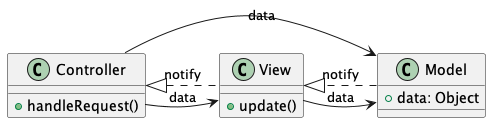
\includegraphics[width=0.8\textwidth]{fig/uml/default-mvc.png}
  \caption{Beispiel eines Basis MVC Architekturmusters}
  \label{fig:default-mvc}
\end{figure}

Diese Basisarchitektur wird nun in ein Fallbeispiel überführt, um verschiedene Aspekte zu diskutieren. Das Szenario für die Fallstudie soll eine einfache Led-Lampe sein, die über eine eigene CPU und eigenen Speicher und einen Bluetooth Sender und Empfänger verfügt. Der Aufbau ist erweitert durch einen Raspberry PI, der sowohl die Anbindung der Lampe über Bluetooth repräsentiert, als auch den Servicezugriffspunkt für Applikationen im Internet. Der Raspberry Pi kann über eine Global Unicast IPv6 Adresse erreicht werden, um Steuerungssignale für die Lampe über die App abzugeben. 

Wir nutzen daher das Architekturmuster um eine Aufteilung in Verantwortlichkeiten zu realisieren. Jede Verantwortlichkeit - des PI, der Lampe und der Nutzerapp - wird in einer Klasse gekapselt. Die Zugehörigkeit zum MVC Pattern wird in diesem Beispiel dadurch Stereotypen zum Ausdruck gebracht.
\\\\
Eine Stereotype ist eine benutzerdefinierte Kennzeichnung eines UML-Elements, die durch das Hinzufügen von Namen, Attributen und Methoden definiert werden kann. Sie erweitern die UML-Notation und ermöglichen es, zusätzliche Informationen oder Bedeutungen einem Element zuzuweisen, ohne die zugrunde liegende UML-Syntax zu ändern. Stereotypen können auch dazu verwendet werden, bestimmte Funktionen oder Verhaltensweisen hinzuzufügen, die von der Basis-UML-Syntax nicht unterstützt werden. Zum Beispiel kann eine Stereotype \enquote{Singleton} einem Klassenobjekt hinzugefügt werden, um anzuzeigen, dass nur eine einzige Instanz dieser Klasse im gesamten System vorhanden sein sollte, oder wie in diesem Fall die Sterotype  \enquote{Model}. Mit Model wird die Klasse Lampe mit der Aufgabe des Buisnessmodells gebunden. 
Die Abbildung~\ref{fig:stereo-mvc} zeigt das sich nun ergebene Bild. 
\begin{figure}[ht]
  \centering
  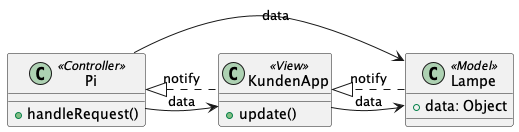
\includegraphics[width=0.8\textwidth]{fig/uml/sterotypen-mvc.png}
  \caption{MVC Architekturmusters im Fallbeispiel mit Sterotypen}
  \label{fig:stereo-mvc}
\end{figure}

Die Aufgaben der einzelnen Komponenten eines MVC-Architekturpatterns sind aber nicht trennscharf und sind wirklich einzig als ein \enquote{Best Practise} Beispiel anzusehen. Die folgende Aufzählung soll nur ein Einblick darin geben, wie weit die Aufgabenfelder der Komponenten erweitert werden, können ohne das MVC-Architekturpattern zu verletzen. 
\begin{itemize}
\item Eine MVC-View kann neben ihrer Hauptfunktion, der Präsentation von Daten, auch weitere Aufgaben übernehmen. Sie kann beispielsweise automatisch die Darstellung von Daten anpassen, wenn Änderungen in den zugehörigen Modellen der Anwendung vorgenommen werden. Zudem kann sie Benutzeraktionen, die über grafische Eingabeelemente wie Textfelder oder Buttons erfolgen, an den Controller weiterleiten. Zusätzlich ist es möglich, dass die View Status- und Fehlermeldungen von Controllern visualisiert.

\item Ein MVC-Controller kann zusätzlich zu seiner Hauptaufgabe, der Steuerung des Datenflusses, weitere Funktionen übernehmen. Er kann beispielsweise Systemsignale wie eine Systemuhr verarbeiten und entsprechend darauf reagieren (z.B. Budget reicht nicht mehr für Nutzung). Zudem kann er die Komponentenlogik der Anwendung umsetzen und die Kommunikation mit externen Datenquellen für den Zweck der Datensynchronisation übernehmen.

\item Ein MVC-Modell kann neben der zentralen Verwaltung von Daten auch anderen Modulen Zugriff auf die Zustandsdaten gewähren und diese über Änderungen informieren, in der Regel mithilfe des Observer-Patterns. Zudem kann es die Komponentenlogik der Anwendung umsetzen und die Kommunikation mit externen Datenquellen koordinieren.
\end{itemize}

\subsubsection{VCM und CVM}
Das MVC Pattern selbst kann auch in unterschiedlichen Schichtenmodellen gedacht werden und in ihrer Ausprägung beispielhaft als VCM und CVM bezeichnet werden.  Es ist wichtig zu beachten, dass VCM und CVM für sich keine weit verbreiteten oder standardisierten Architekturmuster sind und eher als Variationen des MVC-Musters betrachtet werden sollten. Bei den Variationen werden die Reihenfolge der Komponenten verändert und je mit einem Schichtenmodell vereint. Die Abbildung~\ref{fig:mvs-varianten} soll je Ausprägung eine mögliche Interpretation verdeutlichen.

\begin{figure}[ht]
  \centering
  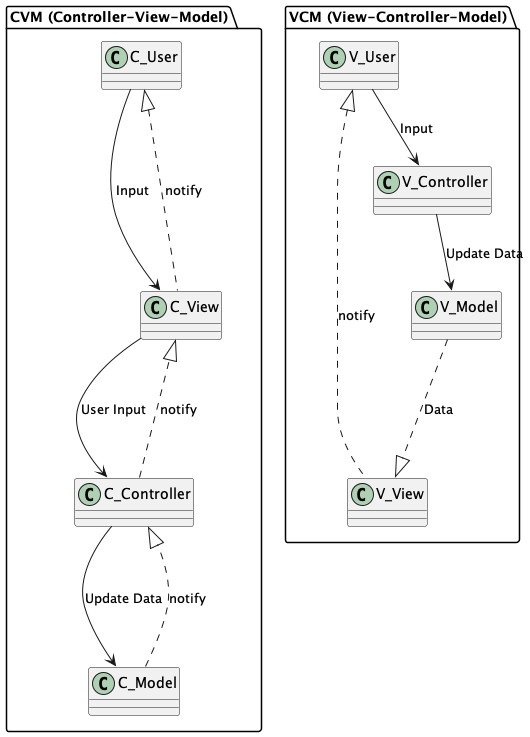
\includegraphics[width=0.65\textwidth]{fig/uml/mvc-varianten.png}
  \caption{Mögliche Varianten vom MVC in Schichten gedacht}
  \label{fig:mvs-varianten}
\end{figure}
Die drei Module einer Model-View-Controller (MVC)-Komponente sind gemäß dem Schichtenparadigma in Ebenen angeordnet. Die höheren Ebenen können auf die tiefergelegenen Ebenen zugreifen, aber nicht umgekehrt. Dies entspricht den Anforderungen an ein gerichtetes Schichtenmodel. 
\\\\
Die unterste Ebene enthält das Modell. Das zugehörige Modul weiß nichts von den über ihm liegenden Modulen und kann mit diesen nur indirekt\footnote{zum Beispiel durch Antworten auf Nachrichten oder mit Hilfe eines sogenannten \enquote{handle} oder \enquote{callback}} kommunizieren.
\\\\
Ein Controllermodul kann direkt auf ein Modellmodul zugreifen, um die Inhalte zu manipulieren. Eine View kommuniziert im Allgemeinen nur direkt mit Controllermodulen, um diesen Benutzeraktionen mitzuteilen.
\\\\
In dem hier vorgestellten Szenario stellt der Benutzer das „oberste Modul“ dar. Es kommuniziert nur gerichtet mit den View- und Controllermodulen. 
\\\\
Wo die in diesem Beispiel aufgebaute CVM Struktur alle Schichten für den Weg zum Modell benutzt und mit dem \enquote{handle} über die Auswirkungen informiert, wird im Beispiel des VCM Model für den Input die Schicht der View Klasse übersprungen, um eine direktere Eingabe zu unterstützen. Somit unterstützt die VCM Struktur das MVC Muster und das Schichtenmodell. Es eignet  sich aber auch für die Verarbeitung von zeitkritischen Inputs, wie sie beispielhaft in einem Jump'n'Run-Spiel gefordert sind. Der besonderer Nachteil ist, es braucht direkte Kommunikationskanäle. Dieser direkte Weg ist aber nicht immer möglich. Auch verlangen Technologien oder auch Frameworks bei User-Inputs nicht selten die klare Trennung von View und Controller. Ein Beispiel für solch eine technologische Anforderung wird von Java FX repräsentiert.     

\paragraph{Beispiel: JavaFX\\\\}
JavaFX ist ein relativ modernes Framework zur Erstellung von graphischen Benutzeroberflächen (GUIs) in Java. Es bietet verbesserte Möglichkeiten im Vergleich zu AWT und Swing. In JavaFX werden Benutzereingaben (User Inputs) über das Event-Handling-System verarbeitet. Hier ist ein Überblick darüber, wie JavaFX mit Benutzereingaben umgeht:
\begin{itemize}
\item Event-Handling: In JavaFX werden Ereignisse (Events) verwendet, um Benutzereingaben wie Mausklicks, Tastaturanschläge und andere Aktionen zu verarbeiten. Jedes Steuerelement (Control) oder Node in JavaFX kann Event-Handler registrieren, um auf spezifische Ereignisse zu reagieren.
\item Event-Typen: JavaFX bietet verschiedene Event-Klassen, die unterschiedliche Arten von Benutzereingaben repräsentieren, z. B. MouseEvent, KeyEvent, ScrollEvent usw. Sie können Event-Handler erstellen, die auf bestimmte Event-Typen reagieren, indem Sie die entsprechenden Methoden überschreiben.
\item Event-Handler: Um auf ein Ereignis zu reagieren, müssen Sie einen Event-Handler erstellen, der eine Methode handle() implementiert, die den Ereignistyp als Parameter akzeptiert. Sie können einen Event-Handler entweder als separate Klasse oder als Lambda-Ausdruck erstellen.
 \end{itemize}   

Das Code-Listing~\ref{lst:javafx-input} macht diese Anforderung dadurch deutlich, das die Java FX Anwendung die \enquote{javafx.application.Application} ableitet. In diesem Beispiel wird ein einfacher Button erstellt, der auf Mausklicks reagiert. Der Event-Handler wird mithilfe eines Lambda-Ausdrucks definiert und beim Klicken des Buttons wird \enquote{Button clicked!} in der Konsole ausgegeben. An dieser Stelle könnten die Daten vom Nutzer auch an den Controller weitergegeben werden.

\subsubsection{Vertreter}
Auch für die Verteilten Systeme machen die Schnittstellen und die Zuordnungen einen wichtigen Unterschied. Jede Bindung der Komponenten bedarf einer Kommunikation, die im Zweifel mit einem Kommunikationsweg  verbunden ist. Dieser Anforderung muss das Overlay- wie auch das physikalische Netzwerk entsprechen. Dies kann weitreichende Entscheidungen mit sich bringen. Stellen wir uns vor, dass die Lampe in unserem Fallbeispiel über Bluetooth angesprochen werden muss, so ist aus der View kein direkter physikalischer Kommunikationsweg vorhanden, um einen \enquote{handle} zu nutzen ohne den Controller oder einen etwaigen Proxy einzusetzen.  Ein Proxy in einem verteilten System ist eine Komponente, die als Vermittler zwischen Clients und entfernten Diensten fungiert. 
\\\\
Der Proxy\index{Proxy} ist eine Art Stellvertreter für den entfernten Dienst und ermöglicht es dem Client, auf diesen Dienst zuzugreifen, als ob er sich lokal im selben Netzwerk befände.
Der Proxy wird typischerweise zwischen dem Consumer und dem entfernten Dienst (Provider) platziert und übernimmt die Verwaltung der Kommunikation zwischen diesen beiden Komponenten. Der Client sendet Anfragen an den Proxy, der die Anfrage entgegennimmt und an den entfernten Dienst weiterleitet. Der entfernte Dienst sendet die Antwort an den Proxy zurück, der die Antwort an den Client weiterleitet.\\\\

\noindent\begin{minipage}{\textwidth}
\begin{lstlisting}[caption={Java FX Input},captionpos=b,label={lst:javafx-input}]
import javafx.application.Application;
import javafx.scene.Scene;
import javafx.scene.control.Button;
import javafx.scene.layout.StackPane;
import javafx.stage.Stage;

public class JavaFXUserInputExample extends Application {

    public static void main(String[] args) {
        launch(args);
    }

    @Override
    public void start(Stage primaryStage) {
        Button button = new Button("Click me!");

        // Registering an EventHandler for the button click
        button.setOnAction(event -> {
            System.out.println("Button clicked!");
        });

        StackPane root = new StackPane();
        root.getChildren().add(button);

        Scene scene = new Scene(root, 300, 250);

        primaryStage.setTitle("JavaFX User Input Example");
        primaryStage.setScene(scene);
        primaryStage.show();
    }
}
\end{lstlisting}
\end{minipage}

Ein Proxy bietet mehrere Vorteile in einem verteilten System. Zum Beispiel kann ein Proxy mit Caching dazu beitragen, die Netzwerklatenz zu reduzieren, indem er Anfragen von Clients bündelt und sie in einer einzigen Anfrage an den entfernten Dienst weiterleitet. Ein Proxy kann auch die Sicherheit erhöhen, indem er den Zugriff auf den entfernten Dienst kontrolliert und Anfragen von unautorisierten Clients blockiert. Das Diagramm \ref{fig:proxy} beschreibt die Idee als Muster von Komponenten:
\begin{figure}[ht]
  \centering
  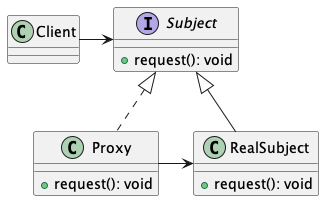
\includegraphics[width=0.45\textwidth]{fig/uml/proxy.png}
  \caption{Proxy Pattern}
  \label{fig:proxy}
\end{figure}
\begin{itemize}
\item \textbf{Client}: Die Klasse, die mit dem Subject-Interface interagiert.
\item \textbf{Subject}: Das Interface, das von Proxy und RealSubject implementiert wird. Es definiert die gemeinsame Schnittstelle für Proxy und RealSubject.
\item \textbf{RealSubject}: Die Klasse, die das eigentliche Objekt repräsentiert, auf das der Proxy zugreifen soll.
\item \textbf{Proxy}: Die Klasse, die den Zugriff auf das RealSubject steuert.
\end{itemize}

Der Client interagiert mit dem Subject-Interface und kennt nicht den Unterschied zwischen Proxy und RealSubject. Der Proxy implementiert das Subject-Interface und steuert den Zugriff auf das RealSubject.
\\\\
Es gibt verschiedene Arten von Proxies, die in einem verteilten System verwendet werden können, wie z.B. Forward Proxy, Reverse Proxy, Caching Proxy und Load Balancing Proxy. Jede Art von Proxy hat ihre eigenen Funktionen und Vorteile, je nach den Anforderungen des Systems und der Architektur:

\begin{itemize}
\item Ein \textbf{Forward Proxy} ist ein Proxy-Server, der als Vermittler zwischen einem Client und dem Internet fungiert. Wenn ein Client eine Anfrage an das Internet sendet, geht die Anfrage zuerst an den Forward Proxy-Server, der dann die Anfrage an das Ziel weiterleitet und die Antwort des Ziels an den Client zurücksendet.

Der Hauptzweck eines Forward Proxys besteht darin, die Privatsphäre und Sicherheit des Clients zu schützen, indem er seine Identität und IP-Adresse vor dem Zielserver verbirgt. Dadurch kann der Client anonym im Internet surfen und verhindern, dass die besuchten Websites seine IP-Adresse oder Identität aufzeichnen.

Forward Proxies werden auch oft in Unternehmen eingesetzt, um den Zugriff auf das Internet zu kontrollieren und zu beschränken. Sie können beispielsweise bestimmte Websites oder Dienste blockieren oder die Verwendung von bestimmten Protokollen einschränken.
\item Im Gegensatz zu einem Forward Proxy, der den Datenverkehr vom Client zu den Servern weiterleitet, empfängt ein \textbf{Reverse Proxy} Anfragen von den Servern und leitet sie an den Client weiter.

Der Hauptzweck eines Reverse Proxys besteht darin, die Last auf die Server zu verteilen, indem er eingehende Anfragen an verschiedene Server weiterleitet, um eine bessere Auslastung und Lastverteilung zu erreichen. Er kann auch zur Beschleunigung der Website-Leistung verwendet werden, indem er häufig angeforderte statische Inhalte im Cache speichert und schneller bereitstellt.

Reverse Proxies werden auch oft als Sicherheitsmaßnahme eingesetzt, um Angriffe auf die Server abzuwehren, indem sie den Server vor direktem Zugriff aus dem Internet schützen und nur autorisierte Anfragen durchlassen.

\item Ein \textbf{Caching Proxy} ist ein Proxy-Server, der den Datenverkehr zwischen einem Client und dem Internet überwacht und häufig abgerufene Inhalte im Cache speichert, um die Website-Leistung zu verbessern und die Belastung der Internetverbindung zu reduzieren.

Wenn ein Client eine Anfrage an das Internet sendet, überprüft der Caching Proxy, ob er eine Kopie der angeforderten Ressource im Cache hat. Wenn dies der Fall ist, wird die Ressource aus dem Cache geladen und an den Client zurückgesendet, ohne dass eine Verbindung zum ursprünglichen Server hergestellt werden muss. Wenn die Ressource nicht im Cache vorhanden ist, leitet der Caching-Proxy die Anfrage an den Server weiter und speichert dann die Antwort im Cache für zukünftige Anforderungen.

Caching-Proxies können dazu beitragen, die Leistung von Websites zu verbessern und die Latenzzeiten zu reduzieren, da häufig angeforderte Ressourcen schneller geladen werden können. Sie können auch dazu beitragen, die Bandbreitennutzung zu reduzieren, da der Proxy den Datenverkehr filtern und nur die notwendigen Ressourcen im Cache speichern kann.
\item Ein \textbf{Load Balancing Proxy} ist ein Proxy-Server, der als Vermittler zwischen einem Client und einem oder mehreren Servern fungiert und die Last auf mehrere Server verteilt, um eine bessere Auslastung und Verfügbarkeit zu erreichen.

Wenn ein Client eine Anfrage an den Load Balancing Proxy sendet, überprüft der Proxy die Server, die die Anfrage bearbeiten können, und leitet die Anfrage dann an den am wenigsten ausgelasteten Server weiter. Dadurch können mehrere Server gleichzeitig Anfragen bearbeiten, wodurch die Leistung und Verfügbarkeit der Anwendung verbessert werden.

Load Balancing Proxies sind besonders nützlich für Websites und Anwendungen mit hohem Traffic oder schweren Workloads, da sie dazu beitragen, die Belastung auf die Server zu reduzieren und eine hohe Verfügbarkeit sicherzustellen. Darüber hinaus können Load Balancing Proxies auch dazu beitragen, die Ausfallsicherheit zu verbessern, da im Falle eines Ausfalls eines Servers die Anfragen automatisch auf einen anderen Server umgeleitet werden können.
\end{itemize}
Ein Proxy ist normalerweise ein Vermittler, der  auf der Netzwerkebene arbeitet und als Gateway zwischen dem Client und dem Server fungiert. Eine Alternative Form zum Proxy kann auch als Broker beschrieben werden. 

Broker und Proxies sind beide Vermittler, die in der Kommunikation zwischen verschiedenen Anwendungen verwendet werden. Der Hauptunterschied zwischen den beiden besteht darin, wie sie diese Kommunikation verarbeiten und welche Funktionen sie bereitstellen.
\\\\
Ein \textbf{Broker} ist ein Vermittler, der die Kommunikation zwischen verschiedenen Anwendungen ermöglicht, indem er Nachrichten empfängt, speichert und an die richtigen Empfänger weiterleitet. Der Broker ist normalerweise in der Lage, die Nachrichten zu filtern, zu transformieren oder zu aggregieren, bevor er sie an den Empfänger weiterleitet. Der Broker kann auch verschiedene Messaging-Protokolle unterstützen und die Nachrichten in einer Warteschlange speichern, wenn der Empfänger nicht verfügbar ist. 

\begin{figure}[ht]
  \centering
  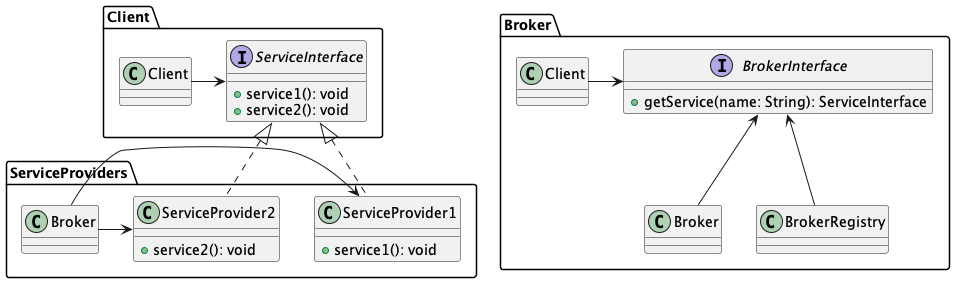
\includegraphics[width=0.95\textwidth]{fig/uml/broker.png}
  \caption{Broker Pattern}
  \label{fig:broker}
\end{figure}

Das Diagramm \ref{fig:broker} beschreibt das Broker-Pattern mit den folgenden Komponenten:
\begin{itemize}
\item \textbf{Client}: Die Klasse, die einen Dienst von einem der Service-Provider anfordert.
\item \textbf{ServiceInterface}: Das Interface, das von den ServiceProvidern implementiert wird. Es definiert die gemeinsame Schnittstelle für die angebotenen Dienste.
\item \textbf{ServiceProvider1, ServiceProvider2}: Die Klassen, die die tatsächlichen Dienste bereitstellen und das ServiceInterface implementieren.
\item BrokerInterface: Das Interface, das von Broker und BrokerRegistry implementiert wird. Es definiert die gemeinsame Schnittstelle, um auf die verschiedenen Dienste zuzugreifen.
\item \textbf{Broker}: Die Klasse, die als Vermittler zwischen Client und ServiceProvider fungiert und die Kommunikation vereinfacht.
\item \textbf{BrokerRegistry}: Die Klasse, die alle verfügbaren ServiceProvider verwaltet und dem Broker bei Bedarf zur Verfügung stellt.
\end{itemize}
Der Client greift über das BrokerInterface auf die gewünschten Dienste zu, ohne direkt mit den ServiceProvider-Klassen zu interagieren. Der Broker verwaltet die Kommunikation zwischen Client und ServiceProvider und entkoppelt so deren Abhängigkeiten.

Es ist weiter möglich eine weitere Unterschiedung in \textbf{Forwarding-Broker} und \textbf{Handle-Driven-Broker} einzuführen. 
\\\\
Ein Forwarding-Broker ist ein Broker, der eingehende Nachrichten an den Empfänger weiterleitet, der von der Nachrichtadresse identifiziert wird. Der Broker hat keine Vorstellung von der Struktur oder dem Inhalt der Nachrichten, sondern dient lediglich als Vermittler zwischen Sender und Empfänger. Es handelt sich um ein sehr einfaches System, das schnell und effizient arbeitet, aber nur minimale Unterstützung für die Transformation von Nachrichten bietet.
\\\\    
Ein Handle-Driven-Broker ist dagegen ein Broker, der Nachrichten auf Basis eines Handles weiterleitet, das als Referenz auf eine Nachricht dient. Der Broker speichert den \enquote{handle} und bietet verschiedene Funktionen an, um die Nachrichten zu bearbeiten oder zu transformieren, bevor sie an den Empfänger weitergeleitet werden. Handle-Driven-Broker bieten erweiterte Funktionen wie die Möglichkeit, Nachrichten zu filtern, zu transformieren oder zu aggregieren, bevor sie an den Empfänger weitergeleitet werden.
\\\\
Auch der Broker kann im Funktionssatz nochmals in einem \textbf{Trader} erweitert werden. Ein Trader ist in einem verteilten System ein Teilnehmer, der versucht, bestimmte Dienste nach Regeln zu suchen oder anzubieten. Trader bieten eine Art von \enquote{Gelbe Seiten} für verteilte Dienste an, in denen sie Informationen wie Dienstbeschreibungen, Verfügbarkeit und Qualitätsmetriken speichern und veröffentlichen. Wenn ein Teilnehmer einen Dienst benötigt, sucht er nach einem passenden Trader und sucht dann nach einem geeigneten Dienst in den bereitgestellten Informationen. Als Pattern ist der Trader eher als Service Locator Pattern bekannt welches im Grundsatz aber sehr ähnlich zu dem Broker Pattern ist. 
\\\\
Das Wichtigste ist aber fernab aller Konnektivität die Umsetzung der \enquote{handle}, ob im direkten Zugriff oder über einen Vermittler. Für die Umsetzung von \enquote{handle} und für die Bindung von Schichten können unterschiedliche Ansätze genutzt werden, eine sehr verbreitete ist das Observer Pattern. 

\subsubsection{Observer Pattern}
In der Grundüberlegung des MVC ist das System eng gekoppelt und soll Änderungen im System immer unmittelbar signalisieren. Als Beispiel kann hier die Aktualisierung des Modells und die Implikation auf die View angesprochen werden. 
Wenn beispielhaft die Lampe angeschaltet wurde, soll das Ereignis auch unmittelbar auf der KundenApp angezeigt werden. 
Diese unmittelbare Kommunikation kann mit einem Observer-Pattern umgesetzt werden. 
\\\\
Das Observer Pattern ist ein Entwurfsmuster, das verwendet wird, um eine 1:n-Beziehung zwischen Objekten zu erstellen, wobei Änderungen an einem Objekt automatisch an andere Objekte weitergegeben werden. Das bedeutet, dass ein Objekt (das sogenannte Subjekt) alle seine Beobachter (die Observer) benachrichtigt, wenn sich sein Zustand ändert. Die Beobachter reagieren dann auf diese Änderung entsprechend.

Das Observer Pattern wird oft in Situationen eingesetzt, in denen es wichtig ist, dass eine Änderung an einem Objekt die darauf basierenden Objekte informiert und automatisch aktualisiert. Zum Beispiel kann ein Nachrichtendienst ein Subjekt sein, das Nachrichten an viele Abonnenten weiterleitet. Ein weiteres Beispiel wäre ein Diagramm, das automatisch aktualisiert wird, wenn sich die zugrunde liegenden Daten ändern. Es kann aber auch eine Middleware sein, die versucht eine oder mehrere Implementierung zu adressieren, um einen entfernen Funktionsaufruf durchzuführen. 
\\\\
Das Observer Pattern besteht aus einem Subjekt, das eine Liste von Beobachtern hält, sowie einer Schnittstelle, die es Beobachtern ermöglicht, auf Änderungen zu reagieren. Wenn sich der Zustand des Subjekts ändert, wird diese Änderung an alle Beobachter übermittelt. Die Beobachter können dann auf diese Änderung reagieren und ihre eigenen Aktionen durchführen.
\begin{figure}[ht]
  \centering
  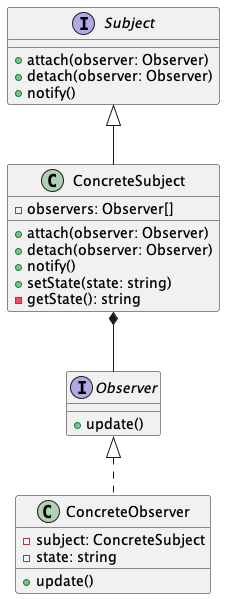
\includegraphics[width=0.25\textwidth]{fig/uml/default-observer.png}
  \caption{Einfaches Observer Pattern}
  \label{fig:default-observer}
\end{figure}

Das Observer Pattern ermöglicht eine flexible und erweiterbare Architektur, da Subjekte und Beobachter unabhängig voneinander implementiert werden können. Subjekte können Beobachter hinzufügen oder entfernen, ohne dass dies Auswirkungen auf den Rest des Systems hat. Beobachter können ebenfalls hinzugefügt oder entfernt werden, ohne dass Änderungen an anderen Teilen des Systems vorgenommen werden müssen.
\\\\
Die Abbildung~\ref{fig:default-observer} zeigt das Observer Pattern mit drei Komponenten: Subject, Observer und ConcreteSubject. Das Subject ist eine Schnittstelle, die von den Subjekten implementiert wird, die beobachtet werden sollen. Es definiert Methoden zum Hinzufügen, Entfernen und Benachrichtigen von Beobachtern. Der Observer ist eine Schnittstelle, die von allen Beobachtern implementiert wird, und definiert eine Methode zum Aktualisieren des Beobachters, wenn sich der Zustand des Subjekts ändert.

Der ConcreteSubject ist das Subjekt, das beobachtet werden soll. Es hält eine Liste von Beobachtern und implementiert die Methoden zum Hinzufügen, Entfernen und Benachrichtigen von Beobachtern. Der ConcreteObserver ist ein Beobachter, der den Zustand des Subjekts aktualisiert, wenn sich dieser ändert.
\\\\
Das Observer Pattern ermöglicht eine lose Kopplung zwischen Subjekten und Beobachtern, da Subjekte nicht von spezifischen Beobachtern abhängig sind und Beobachter nicht von spezifischen Subjekten. Man beachte, dass eine lose Kopplung zwischen den Komponenten gelingt, aber eine enge Kopplung bei der Kommunikation unterstützt wird. 
\\\\
Für unser Anwendungsbeispiel angepasst, soll das Oberver-Pattern zwischen der KundenApp (View) und der Lampe (Model) etabliert werden. Eine vereinfachte Architektur könnte wie in Abbildung~\ref{fig:mvc-observer} aufgebaut werden. 

\begin{figure}[ht]
  \centering
  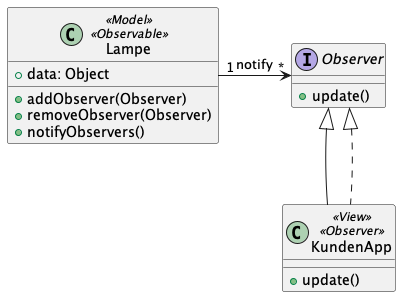
\includegraphics[width=0.45\textwidth]{fig/uml/mvc-observer.png}
  \caption{Observer Pattern als Verbindung zwischen Model und View}
  \label{fig:mvc-observer}
\end{figure}

Natürlich ist ein Architektur-Modell nicht ausreichend, um das gesamte Design zu beschreiben, auch das MVC Architektur-Modell braucht weitere Informationen für das vollständige System. Eine wichtige zusätzliche Information ist das Verhalten der Architektur. Auch für dieses Verhalten bestehen \enquote{Best Practise} Ansätze, die wir als Verhaltensmuster (Behavioral Patterns) beschreiben. 
\\\\
\textbf{Verhaltensmuster} (Behavioral Patterns) sind Entwurfsmuster in der Softwareentwicklung, die sich mit der Organisation und Steuerung von Objekten und deren Interaktionen beschäftigen. Sie beschreiben, wie verschiedene Objekte zusammenarbeiten und wie sie Verhaltensweisen und Aufgaben koordinieren.
\\\\
Behavioral Patterns beschreiben das Verhalten von Objekten in bestimmten Situationen und stellen somit Lösungen für wiederkehrende Probleme bereit, wie z.B. die Steuerung von Abläufen, die Verwaltung von Zuständen oder die Behandlung von Fehlern. Es gibt verschiedene Arten von Behavioral Patterns, die je nach Art der Aufgabe, die sie lösen sollen, in verschiedene Kategorien unterteilt werden können:
\begin{itemize}
\item \textbf{Klassifizierungsmuster} (Classification Patterns): Diese Muster beschreiben, wie Objekte in Klassen und Kategorien organisiert werden können, um eine effektive Klassifizierung und Strukturierung von Objekten zu ermöglichen. Ein Beispiel für ein solches Muster ist das Strategy Pattern.
\item \textbf{Kommunikationsmuster} (Communication Patterns): Diese Muster beschreiben, wie Objekte miteinander kommunizieren und wie Nachrichten oder Daten zwischen ihnen ausgetauscht werden können. Ein Beispiel für ein solches Muster ist das Observer Pattern.
\item \textbf{Kontrollmuster} (Control Patterns): Diese Muster beschreiben, wie Objekte kontrolliert und gesteuert werden können, um eine effektive Durchführung von Abläufen und Prozessen zu ermöglichen. Ein Beispiel für ein solches Muster ist das Command Pattern.
\item \textbf{Datenmuster} (Data Patterns): Diese Muster beschreiben, wie Daten zwischen Objekten ausgetauscht und gespeichert werden können. Ein Beispiel für ein solches Muster ist das Iterator Pattern.
\end{itemize}
Es ergibt sich natürlich, dass die Kommunikationsmuster eine besondere Bedeutung in dem Design eines verteilten Systems einnehmen. 
\\\\
Für die Beschreibung von Behavioral Patterns eignen sich in UML (Unified Modeling Language) vor allem die folgenden Diagrammtypen:
\begin{itemize}
\item \textbf{Aktivitätsdiagramme} (Activity Diagrams): Diese Diagramme werden verwendet, um die Abläufe und Prozesse in einem System oder einer Anwendung zu beschreiben. Aktivitätsdiagramme können verwendet werden, um die Interaktionen zwischen verschiedenen Objekten in einem Behavioral Pattern darzustellen.
\item \textbf{Sequenzdiagramme} (Sequence Diagrams): Diese Diagramme werden verwendet, um die Interaktionen zwischen verschiedenen Objekten in einer bestimmten Sequenz darzustellen. Sequenzdiagramme können verwendet werden, um die Kommunikationsmuster in einem Behavioral Pattern zu beschreiben.
\item \textbf{Zustandsdiagramme} (State Diagrams): Diese Diagramme werden verwendet, um den Zustand eines Objekts und die Übergänge zwischen verschiedenen Zuständen zu beschreiben. Zustandsdiagramme können verwendet werden, um die Kontrollmuster in einem Behavioral Pattern zu beschreiben.
\item \textbf{Interaktionsübersichtsdiagramme} (Interaction Overview Diagrams): Diese Diagramme werden verwendet, um die Interaktionen zwischen verschiedenen Objekten und deren Kommunikationsmuster in einem System oder einer Anwendung zu beschreiben. Interaktionsübersichtsdiagramme können verwendet werden, um eine Übersicht über die Interaktionen in einem Behavioral Pattern zu geben.
\end{itemize}
Durch die Verwendung dieser Diagrammtypen können Behavioral Patterns effektiv beschrieben und visualisiert werden, was zu einer verbesserten Verständlichkeit und Kommunikation der Konzepte und Strukturen innerhalb des Patterns führt.
\\\\
In dem Fallbeispiel der Lampe soll zur Verdeutlichung die einfache Sequenz des Hinzufügen eines Observers zwischen PI (Controller) und Lampe (Model) den Nutzen verdeutlichen. 

\begin{figure}[ht]
  \centering
  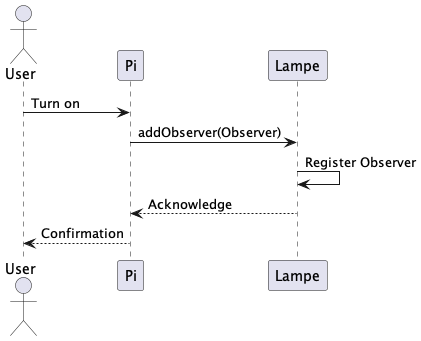
\includegraphics[width=0.55\textwidth]{fig/uml/seq-mvc-observer.png}
  \caption{Observer Pattern als Verbindung zwischen Model und View}
  \label{fig:seq-mvc-observer}
\end{figure}

Im Sequenzdiagramm~\ref{fig:seq-mvc-observer} sind die Schritte zum Hinzufügen eines Observers wie folgt beschrieben:
\begin{itemize}
\item Der Benutzer initiiert den Prozess, indem er den Controller bittet, einen neuen Observer hinzuzufügen.
\item Der Controller ruft die \enquote{addObserver()} Methode des Models auf und übergibt den Observer als Parameter.
\item Das Model registriert den neuen Observer intern, z.B. indem es ihn in einer Liste von Beobachtern speichert.
\item Nachdem der Observer erfolgreich registriert wurde, bestätigt das Model dies dem Controller.
\item Schließlich bestätigt der Controller dem Benutzer, dass der Observer erfolgreich hinzugefügt wurde.
\end{itemize}
Dieses Sequenzdiagramm zeigt die Interaktionen zwischen Benutzer, Controller, Model und Observer beim Hinzufügen eines Observers im Kontext eines MVC-Architekturmusters bei der Initialisierung des Systems. Es ist sicherlich schnell zu erkennen, das weder das Behavioral Pattern noch das Architecture Pattern alleine ausreichend Informationen bietet. Nur in gegenseitiger Ergänzung bieten sie ein vollständiges Bild. Dem geneigten Leser ist es in diesem Fall als Übung überlassen, die Architektur mit dem Observer zwischen Pi und Lampe zu beschreiben, wie das Verhalten an der Schnittstelle Lampe und KundenApp. 
\\\\
Ob das MVC-Pattern mit einer Kopplung über das Observer Pattern gelingt, ist nicht nur ein Design, sondern auch eine Technologie-abhängige Fragestellung. Das Observer Pattern verlangt die Möglichkeit einer unabhängigen uni-direktionalen Kommunikation zwischen dem Subjekt und den Beobachtern, die nur in eine Richtung erfolgt. Dies ist sowohl in einem Programmstack möglich, als auch bei der klassischen Socket-Kommunikation. Beispielhaft ist TCP ein Transportprotokoll auf Layer 4 des ISO-OSI Referenzmodells, welches als Schnittstelle über die Socket-API den Entwicklern bereitgestellt wird. Mit einem Applikations-Protokoll, das diese Eigenschaften nutzt, ist eine Umsetzung des Observer-Patterns eine gute Wahl. 
\\\\
% TODO Check spell
In klassischen Web-Applikationen\footnote{Gemeint sind klassiche Client-Server Anwendungen, Keine ReSTful-etablierten Microservices mit beispielsweise Spring}, selbst wenn sie auf UDP oder TCP basieren, ist dies ohne weiteres nicht der Fall. Als Beispiel kann das HTTP Protokoll herangezogen werden, das auf Basis von TCP ein zustandloses Protokoll anbietet und zudem dem Request-Response-Cycle unterliegt. Insbesondere der Request-Response-Cycle setzt für jede Anfrage eine Antwort voraus und widerspricht der Funktionsweise des Observer Patterns.
\\\\
In der Praxis können Techniken wie WebSockets oder Long Polling verwendet werden, um eine Art Zustand und damit unabhängiger Kommunikation zwischen Subjekt und den Beobachtern zu simulieren und das Observer-Pattern zu verwenden, dennoch sind diese Lösungen nicht Teil von älteren HTTP Standards und sind zudem in Teilen sehr fehleranfällig. Zur Erklärung, bei diesen Lösungen werden Verbindungen zwischen Subjekt und dem Beobachter aufrechterhalten und bei Zustandsänderungen werden die entsprechenden Beobachter benachrichtigt. Allerdings sind diese Techniken mit erhöhtem Aufwand verbunden und haben auch andere Nachteile, wie z.B. eine höhere Netzwerklast und eine höhere Komplexität in der Implementierung. 
Auch werden in unterschiedlichen HTTP Versionen unterschiedlichen \enquote{Workarounds} angeboten. So können bei HTTP2/ HTTP3 Technologien wie Server-Push Mechanismen genutzt werden. Diese werden aber stark im Kontext der Sicherheit diskutiert. 
\\\\
Neben dem Observer Pattern, sieht man in Verteilten Systemen auch immer wieder das Callback Pattern eingesetzt, da es nur einfache Kommunikationsstrukturen braucht. In Situationen, in denen nur eine einzige Funktion oder ein einziges Objekt auf ein bestimmtes Ereignis reagieren muss, bietet daher das Callback-Pattern eine einfachere und leichter verständliche Implementierung.

Das Callback-Pattern ist auch nützlich, wenn es darum geht, den Programmfluss nicht zu blockieren, insbesondere bei asynchronen oder zeitintensiven Operationen. Es ermöglicht die Ausführung anderer Aufgaben, während die lang andauernde Operation im Hintergrund abläuft, und die Callback-Funktion wird aufgerufen, sobald die Operation abgeschlossen ist.

\subsubsection{Callback Pattern}
Das Callback-Pattern ist ein Verhaltensmuster in der Softwareentwicklung, bei dem eine Funktion (auch als Methode oder Prozedur bezeichnet) als Argument an eine andere Funktion übergeben wird. Diese übergebene Funktion, die als Callback-Funktion bezeichnet wird, wird zu einem späteren Zeitpunkt, oft nach Abschluss einer bestimmten Aufgabe oder einem Ereignis, vom aufrufenden Code ausgeführt. Das Callback-Pattern wird häufig verwendet, um asynchrone Programmierung, Ereignisbehandlung oder die Entkopplung von Funktionen zu ermöglichen und eignet sich somit auch für die asynchrone Kommuniaktation in einem verteilten System.
\begin{figure}[ht!]
  \centering
  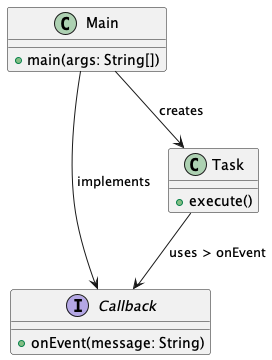
\includegraphics[width=0.30\textwidth]{fig/uml/callback-class.png}
  \caption{Callback Pattern}
  \label{fig:callback-class}
\end{figure}

\begin{figure}[ht!]
  \centering
  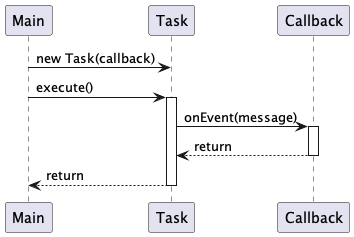
\includegraphics[width=0.50\textwidth]{fig/uml/callback-seq.png}
  \caption{Callback Pattern Sequenz}
  \label{fig:callback-seq}
\end{figure}

In den Diagrammen ~\ref{fig:callback-class} und ~\ref{fig:callback-seq} wird das Callback-Pattern über die Callback-Schnittstelle, die Task-Klasse und die Main-Klasse dargestellt. Die Callback-Schnittstelle definiert die Methode onEvent(), die später als Callback-Funktion verwendet wird. Die Task-Klasse enthält die execute()-Methode, die die Callback-Funktion aufruft, wenn eine bestimmte Aktion oder ein bestimmtes Ereignis eintritt. Schließlich erstellt die Main-Klasse sowohl ein Task-Objekt als auch eine Implementierung der Callback-Schnittstelle und stellt die Kommunikation zwischen diesen beiden Elementen her. Dies ist im folgenden Listing zu erkennen.\\\\

\noindent\begin{minipage}{\textwidth}
\begin{lstlisting}[caption={Callback Pattern},captionpos=b,label={lst:callback}]
// Callback-Interface
interface Callback {
    void onEvent(String message);
}

// Klasse, die die Callback-Funktion verwendet
class Task {
    private Callback callback;

    public Task(Callback callback) {
        this.callback = callback;
    }

    public void execute() {
        // ... fuehre einige Aktionen aus
        callback.onEvent("Task abgeschlossen");
    }
}

// Hauptklasse
public class Main {
    public static void main(String[] args) {
        Callback callback = message -> System.out.println("Callback erhalten: " + message);
        Task task = new Task(callback);
        task.execute();
    }
}
\end{lstlisting}
\end{minipage}
Obwohl Callback Pattern und Observer Pattern beide Techniken zur Implementierung von ereignisgesteuerten Kommunikationen zwischen Objekten sind, gibt es einige wichtige Unterschiede zwischen ihnen:

\begin{itemize}
\item Die aufgerufene Funktion oder das aufgerufene Objekt führt die übergebene Callback-Funktion unter bestimmten Bedingungen aus (z.B. nachdem eine bestimmte Aktion abgeschlossen ist). Ein Observer Pattern informiert über Änderungen oder Ereignisse.
\item Das Callback Pattern ermöglicht eine einfache, unidirektionale Kommunikation zwischen zwei Objekten oder Funktionen. Die Kommunikationsbeziehung bei Observer Pattern ist $1:n$. 
\item Das Callback Pattern eignet sich gut für einfache und direkte Kommunikationsanforderungen, bei denen nur eine geringe Anzahl von Funktionen oder Objekten beteiligt ist. Das Observer Pattern ermöglicht eine lose Kopplung zwischen Objekten und ist skalierbar, da eine beliebige Anzahl von Observern benachrichtigt werden kann.
\end{itemize}\
Im Listing~\ref{lst:callback} und Listing~\ref{lst:observer-I},~\ref{lst:observer-II} ist zu sehen, wie das Callback Pattern und das Observer Pattern in Java-Code implementiert werden. Im Callback Pattern wird eine Funktion direkt an die ausführende Klasse (Task) übergeben, während im Observer Pattern die Observer sich beim Subject (auch Task in diesem Beispiel) registrieren, um Benachrichtigungen zu erhalten.

Für Verteilte Systeme ist sowohl für das Observer Pattern als auch das Callback Pattern die Referenzen des Callbacks bzw. des Observers eine Herausforderung. Da Verteilte Systeme sich keinen gemeinsamen Speicher teilen, muss ein Ersatz für die Adressierung der Referenz gefunden werden, dies soll zu einem späteren Zeitpunkt diskutiert werden. \\

\begin{minipage}{\textwidth}
\begin{lstlisting}[caption={Observer Pattern - ConcreteSubject},captionpos=b,label={lst:observer-I}]
import java.util.ArrayList;
import java.util.List;

// Subject-Interface
interface Subject {
    void addObserver(Observer observer);
    void removeObserver(Observer observer);
    void notifyObservers();
}

// Observer-Interface
interface Observer {
    void update(String message);
}

// ConcreteSubject
class Task implements Subject {
    private List<Observer> observers = new ArrayList<>();
    private String message;

    public void execute() {
        // ... fuehre einige Aktionen aus
        message = "Task abgeschlossen";
        notifyObservers();
    }

    @Override
    public void addObserver(Observer observer) {
        observers.add(observer);
    }

    @Override
    public void removeObserver(Observer observer) {
        observers.remove(observer);
    }

    @Override
    public void notifyObservers() {
        for (Observer observer : observers) {
                     observer.update(message);
        }
    }
}


\end{lstlisting}
\end{minipage}

Neben der Kommunikation der Komponenten, die zudem noch in eine Uni- oder Mulitcast Kommunikation unterschieden werden kann, muss auch die Initialisierung für verteilte Systeme diskutiert werden. In diesem Skript sollen neben den Singleton und den Factory Pattern auch die Initialisierung mit Dependency Injection besprochen werden.\\\\
\begin{minipage}{\textwidth}
\begin{lstlisting}[caption={Observer Pattern - Concrete Observer},captionpos=b,label={lst:observer-II}]
// ConcreteObserver
class TaskObserver implements Observer {
    private String observerName;

    public TaskObserver(String observerName) {
        this.observerName = observerName;
    }

    @Override
    public void update(String message) {
        System.out.println(observerName + " hat eine Benachrichtigung erhalten: " + message);
    }
}

// Hauptklasse
public class Main {
    public static void main(String[] args) {
        Task task = new Task();
        TaskObserver observer1 = new TaskObserver("Observer1");
        TaskObserver observer2 = new TaskObserver("Observer2");

        task.addObserver(observer1);
        task.addObserver(observer2);

        task.execute();

        task.removeObserver(observer1);

        task.execute();
    }
}
\end{lstlisting}
\end{minipage}

\subsubsection{Singleton Pattern}

Das Singleton-Pattern ist ein Entwurfsmuster, das sicherstellt, dass eine Klasse nur eine einzige Instanz hat und einen globalen Zugriffspunkt zu dieser Instanz bereitstellt. In verteilten Systemen kann die Verwendung des Singleton-Patterns einige Herausforderungen mit sich bringen, da es mehrere Knoten oder Prozesse gibt, die möglicherweise auf die Singleton-Instanz zugreifen müssen.
\begin{figure}[!ht]
  \centering
  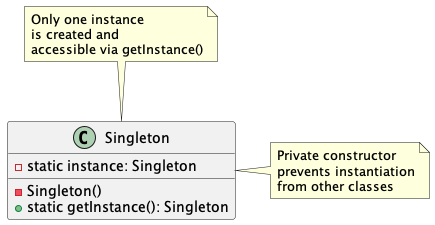
\includegraphics[width=0.45\textwidth]{fig/uml/singleton.png}
  \caption{Singleton Pattern}
  \label{fig:singleton}
\end{figure}

In dem Diagramm~\ref{fig:singleton} gibt es eine Singleton-Klasse, die das Singleton-Pattern implementiert. Die Klasse hat:
\begin{itemize}
\item Eine private statische Variable instance, die die einzige Instanz der Singleton-Klasse speichert.
\item Einen privaten Konstruktor (Singleton()), der die Erstellung von Instanzen der Singleton-Klasse von außen verhindert.
\item Eine öffentliche statische Methode getInstance(), die die einzige Instanz der Singleton-Klasse zurückgibt oder bei Bedarf erstellt.
\end{itemize}
Die Anmerkungen im Diagramm verdeutlichen, dass der private Konstruktor die Instanziierung von anderen Klassen verhindert und dass nur eine Instanz der Singleton-Klasse erstellt und über die getInstance()-Methode zugänglich gemacht wird.
\begin{itemize}
\item Ressourcenverwaltung: Das Singleton-Pattern kann bei der Verwaltung von Ressourcen, wie zum Beispiel Verbindungen zu Datenbanken oder Diensten, nützlich sein. Es kann dazu beitragen, den Ressourcenverbrauch zu minimieren, indem es verhindert, dass mehrere Verbindungen oder Instanzen erstellt werden, die dieselben Ressourcen verwenden.
\item Zentrale Steuerung: Ein Singleton kann als zentrale Steuerungs- oder Koordinationskomponente in einem verteilten System dienen, indem es sicherstellt, dass es nur eine einzige Instanz gibt, die den globalen Zustand verwaltet. Ein Singleton-Pattern kann für verschiedene Anforderungen in einem verteilten System unterschiedliche Auswirkungen haben. Einige sollen exemplarisch diskutiert werden.
\end{itemize}
\begin{itemize}
\item Skalierbarkeit: Das Singleton-Pattern kann die Skalierbarkeit eines verteilten Systems beeinträchtigen, da alle Knoten oder Prozesse auf die einzelne Instanz des Singleton-Objekts zugreifen müssen. Dadurch kann es zu Engpässen oder Leistungsproblemen kommen, wenn die Anzahl der Knoten oder Prozesse zunimmt.
\item Synchronisation: In verteilten Systemen kann die Synchronisation von Singleton-Instanzen eine Herausforderung darstellen. Um sicherzustellen, dass alle Knoten dieselbe Singleton-Instanz verwenden, muss ein Mechanismus implementiert werden, um den globalen Zustand der Instanz konsistent zu halten. Dies kann zusätzliche Komplexität und Overhead verursachen, insbesondere wenn das verteilte System auch fehlertolerant sein muss.
\item Fehlertoleranz: Ein Singleton-Objekt kann in einem verteilten System zu einem Single Point of Failure (SPOF) werden. Wenn die Singleton-Instanz ausfällt, kann dies das gesamte System beeinträchtigen. Um dieses Problem zu umgehen, sind zusätzliche Maßnahmen wie Replikation oder Clustering erforderlich, die die Komplexität erhöhen und möglicherweise die Vorteile des Singleton-Patterns zunichte machen.
\end{itemize}
Im Kontext dieser Diskussion kann festgestellt werden, das die Eignung des Singleton-Patterns in verteilten Systemen von den spezifischen Anforderungen und der Architektur des Systems abhängt. 

\subsubsection{Factory Pattern}
Das Factory-Pattern ist ein Entwurfsmuster, das Objekterstellung auf eine separate Factory-Klasse auslagert. Dies ermöglicht die Erstellung von Objekten, ohne dass der Client-Code direkt den Konstruktor der Objekte aufrufen muss. In verteilten Systemen kann das Factory-Pattern einige Vorteile bieten, welche erneut an einigen Beispielen diskutiert werden soll:
\begin{itemize}
\item Abstraktion und Entkopplung: Das Factory-Pattern hilft, den Client-Code von den konkreten Implementierungsdetails der erstellten Objekte zu entkoppeln. In verteilten Systemen kann dies besonders nützlich sein, da Änderungen an den Implementierungen von Diensten oder Komponenten ohne Auswirkungen auf den Client-Code vorgenommen werden können. Dies erleichtert die Wartung und Skalierung des Systems.
\item Flexibilität bei der Objekterstellung: Das Factory-Pattern ermöglicht es, verschiedene Implementierungen von Objekten zu erstellen, basierend auf der Systemkonfiguration oder den Anforderungen des verteilten Systems. Dies kann dazu beitragen, dass das System einfacher an unterschiedliche Umgebungen oder Anforderungen angepasst werden kann.
\item Vereinfachung der Objekterstellung: In verteilten Systemen kann die Erstellung von Objekten, insbesondere von Ressourcen wie Verbindungen zu Datenbanken oder externen Diensten, komplex sein. Das Factory-Pattern kann dazu beitragen, diese Komplexität zu kapseln und die Erstellung von Objekten für den Client-Code zu vereinfachen. Dadurch wird der Code leichter verständlich und wartbar.
\item Zentrale Verwaltung von Ressourcen: In verteilten Systemen kann die Verwaltung von Ressourcen wie Verbindungen oder Diensten eine Herausforderung darstellen. Durch die Verwendung des Factory-Patterns können diese Ressourcen zentral erstellt und verwaltet werden, was zu einer besseren Kontrolle und einem effizienteren Ressourcenmanagement führt.
\item Load Balancing und Failover: Das Factory-Pattern kann in verteilten Systemen dazu verwendet werden, Load Balancing und Failover-Mechanismen zu implementieren. Die Factory kann die Anfragen auf verschiedene Knoten oder Instanzen verteilen, um die Last auszugleichen oder im Falle eines Ausfalls auf einen anderen Knoten umzuschalten. Dies trägt zur Skalierbarkeit und Fehlertoleranz des Systems bei.
\end{itemize}
\begin{figure}[!ht]
  \centering
  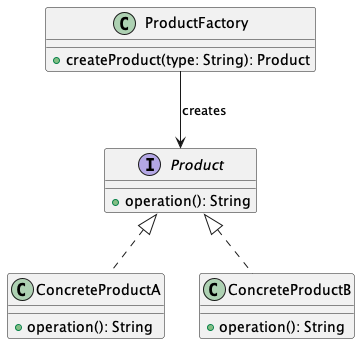
\includegraphics[width=0.45\textwidth]{fig/uml/factory-class.png}
  \caption{Factory Pattern}
  \label{fig:factory-class}
\end{figure}
Das Diagramm~\ref{fig:factory-class} beschreibt das Factory Pattern.
\begin{itemize}
\item Ein Product-Interface, das die gemeinsame Schnittstelle für alle Produkte definiert.
\item Zwei konkrete Produktklassen (ConcreteProductA und ConcreteProductB), die das Product-Interface implementieren. Sie stellen unterschiedliche Produktvarianten dar.
\item Eine ProductFactory-Klasse, die für die Erstellung von Product-Objekten verantwortlich ist.
\end{itemize}
Das Factory-Pattern kapselt die Logik zur Erstellung von Produktobjekten in der ProductFactory-Klasse. Der Client-Code verwendet die createProduct()-Methode der Factory, um ein Produktobjekt zu erstellen, ohne sich um die konkreten Implementierungsdetails der Produktklassen kümmern zu müssen. Das Diagramm zeigt, dass die ProductFactory-Klasse das Product-Interface verwendet, um Produktobjekte zu erstellen, wobei die konkreten Produktklassen die Implementierung bereitstellen.

\begin{figure}[!ht]
  \centering
  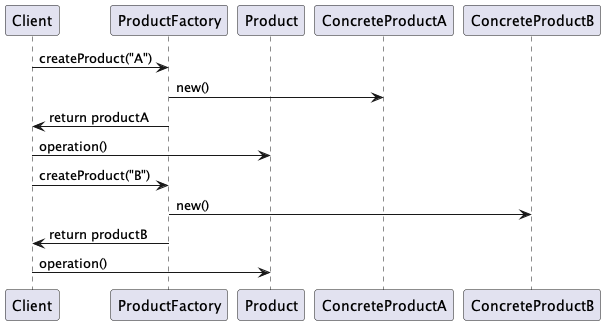
\includegraphics[width=0.85\textwidth]{fig/uml/factory-seq.png}
  \caption{Factory Pattern Sequenz}
  \label{fig:factory-seq}
\end{figure}

Das Factory-Pattern in verteilten Systemen bieter darüber hinaus eine Reihe von Vorteilen, die dazu beitragen, den Code sauberer und wartbarer zu gestalten Wie auch immer, obwohl das Factory-Pattern in vielen verteilten Systemen Vorteile bietet, gibt es auch Situationen, in denen Probleme auftreten können. Einige sind im Folgenden angesprochen:
\begin{itemize}
\item Kommunikationslatenz: In verteilten Systemen kann die Kommunikation zwischen den Knoten und den Factory-Instanzen Latenz verursachen. Wenn der Factory-Code auf einem zentralen Knoten gehostet wird, kann dies zu Verzögerungen bei der Objekterstellung führen und die Gesamtleistung des Systems beeinträchtigen.
\item Synchronisation: In verteilten Systemen kann die Synchronisation der Factory-Instanzen über mehrere Knoten hinweg eine Herausforderung darstellen. Wenn der Factory-Code oder die Konfigurationsinformationen geändert werden, müssen alle Factory-Instanzen im System aktualisiert werden, um konsistent zu bleiben. Dies kann zu zusätzlicher Komplexität und möglichen Inkonsistenzen führen.
\item Single Point of Failure (SPOF): Wenn die Factory zentral verwaltet wird oder auf einem einzelnen Knoten gehostet ist, kann dies zu einem Single Point of Failure führen. Im Falle eines Ausfalls dieses Knotens oder der Factory-Instanz kann das gesamte verteilte System beeinträchtigt werden. Um dieses Risiko zu minimieren, sind möglicherweise zusätzliche Maßnahmen wie Replikation oder Clustering erforderlich.
\item Erhöhte Komplexität: Obwohl das Factory-Pattern dazu beitragen kann, die Komplexität der Objekterstellung zu reduzieren, kann es in einigen Fällen auch zusätzliche Komplexität in das verteilte System einführen. Die Implementierung von Factories, die auf verschiedenen Knoten verteilt sind, kann die Systemarchitektur und das Debugging komplexer gestalten. In solchen Fällen kann es schwieriger sein, den Überblick über den Datenfluss und die Abhängigkeiten zwischen den Knoten zu behalten.
\item Schwerer zu testen: In verteilten Systemen kann das Testen von Factory-Implementierungen aufgrund der beteiligten Knoten und der möglichen Latenz- oder Synchronisationsprobleme schwieriger sein. Die Testbarkeit von Factories und den erstellten Objekten kann in solchen Umgebungen eingeschränkt sein, was zu einer geringeren Codequalität führen kann.
\item Overhead: Die Verwendung von Factories in verteilten Systemen kann zusätzlichen Overhead verursachen, insbesondere wenn die Objekterstellung häufig stattfindet oder eine große Anzahl von Knoten beteiligt ist. In solchen Fällen kann der zusätzliche Overhead, der durch die Kommunikation zwischen den Knoten und der Factory entsteht, die Leistung des Systems beeinträchtigen.
\end{itemize}

Trotz dieser Herausforderungen und Probleme ist das Factory-Pattern eine wichtige Option in der Architektur eines verteilten Systems sein. 

\subsubsection{Dependency Injection Pattern}

Das Dependency Injection (DI) Pattern ist ein Entwurfsmuster, bei dem die Abhängigkeiten eines Objekts von außen bereitgestellt werden, anstatt dass das Objekt sie selbst erstellt. Dies kann helfen, den Code modularer, testbarer und wartbarer zu gestalten. Es kann wie folgt angewendet werden:
\begin{itemize}
\item Definieren Sie Schnittstellen oder abstrakte Klassen für die Abhängigkeiten, die von den Komponenten des Systems benötigt werden.
\item Implementieren Sie die konkreten Klassen, die diese Schnittstellen oder abstrakten Klassen erfüllen.
\item Verwenden Sie einen DI-Container oder ein Framework (z. B. Spring in Java), um Abhängigkeiten zu konfigurieren, zu erstellen und in die jeweiligen Komponenten zu injizieren.
\item Stellen Sie sicher, dass die Komponenten im System sich nur auf die definierten Schnittstellen oder abstrakten Klassen beziehen, anstatt direkt auf die konkreten Implementierungen zuzugreifen.
\end{itemize}    
Wenn das DI-Pattern in einem verteilten System implementiert ist, können verschiedene Knoten unterschiedliche Implementierungen oder Konfigurationen der Abhängigkeiten verwenden, ohne den Code der einzelnen Komponenten ändern zu müssen. Dies ermöglicht eine größere Flexibilität und Anpassungsfähigkeit des Systems an verschiedene Umgebungen und Anforderungen. Ein Beispiel für das Dependency Injection-Pattern in einem verteilten System könnte ein System mit mehreren Microservices sein, die über ein Netzwerk kommunizieren. Jeder Microservice hat seine eigene Aufgabe und benötigt möglicherweise Zugriff auf verschiedene externe Ressourcen oder Dienste. Anstatt dass jeder Microservice direkt auf diese Ressourcen zugreift, werden die Abhängigkeiten über DI bereitgestellt. Dies ermöglicht es, die Ressourcen zentral zu verwalten und bei Bedarf unterschiedliche Implementierungen oder Konfigurationen bereitzustellen.
\\\\
Um die Funktionsweise des Patterns zu verdeutlichen, soll nochmals das Fallbeispiel mit der Lampe bemüht werden. Der Fokus liegt darauf, dass der Pi (Controller) die Lampe (Model) kontrolliert. 
\\\\
Zunächst erstellen wir eine Schnittstelle für die Abhängigkeit:\\

\noindent\begin{minipage}{\textwidth}
\begin{lstlisting}[caption={Schnittstelle für die Abhängigkeit},captionpos=b,label={lst:di-interface}]
public interface BulbService {
    void doLight();
}
\end{lstlisting}
\end{minipage}

Dann erstellen wir eine Implementierung dieser Schnittstelle:\\
\noindent\begin{minipage}{\textwidth}
\begin{lstlisting}[caption={Schnittstellenimplementierung},captionpos=b,label={lst:di-interface-implementation}]

public class Bulb implements BulbService {
    public void doLight() {
        System.out.println("Do cool Stuff");
    }
}
\end{lstlisting}
\end{minipage}
Als nächstes erstellen wir die Klasse, die die Abhängigkeit benötigt:\\\\
\noindent\begin{minipage}{\textwidth}
\begin{lstlisting}[caption={Dependency},captionpos=b,label={lst:di-dependency}]

public class ControllerOnPI {
    private BulbService service;
    
    public ControllerOnPI(BulbService service) {
        this.service = service;
    }
    
    public void doControl() {
        service.doLight();
    }
}
\end{lstlisting}
\end{minipage}
Hier haben wir eine Konstruktor-basierte Dependency Injection verwendet, um die Abhängigkeit von MessageService in MyApplication zu injizieren.
\\\\
Schließlich können wir unser Beispiel in der Main-Methode verwenden:\\\\
\noindent\begin{minipage}{\textwidth}
\begin{lstlisting}[caption={Die DI Main},captionpos=b,label={lst:di-main}]
public class Main {
    public static void main(String[] args) {
        BulbService bulb = new Bulb();
        ControllerOnPI c = new ControllerOnPI(bulb);
        
        c.doControl();
    }
}
\end{lstlisting}
\end{minipage}

Dependency Injection (DI) ist ein nützliches Muster für die Entwicklung von Anwendungen. Es hat jedoch auch Nachteile, insbesondere in verteilten Systemen. Einer der Nachteile ist, dass DI in verteilten Systemen eine zusätzliche Komplexität einführen kann, insbesondere wenn viele verschiedene Komponenten vorhanden sind, die miteinander kommunizieren müssen. DI kann auch die Leistung beeinträchtigen, insbesondere wenn die Abhängigkeiten zwischen den Komponenten in einem verteilten System über ein Netzwerk übertragen werden müssen. Ein weiterer Nachteil von DI in verteilten Systemen ist, dass es ein Sicherheitsrisiko darstellen kann, wenn es nicht ordnungsgemäß implementiert wird. Außerdem kann DI die Skalierbarkeit beeinträchtigen, wenn die Komponenten in der Anwendung nicht ordnungsgemäß entkoppelt sind. Schließlich kann DI auch das Debugging erschweren, insbesondere wenn es viele verschiedene Komponenten gibt, die miteinander interagieren. Daher müssen diese Nachteile von Dependency Injection berücksichtigt werden, wenn sie in verteilten Systemen eingesetzt wird, um sicherzustellen, dass die Implementierung angemessen ist und die Anforderungen des Systems erfüllt.
\\\\
Dependency Injection (DI) wird häufig mit einem Konzept aus der Programmierung verbunden das Reflections (Reflexion) genannt wird. In der Informatik bezieht sich Reflection (Reflexion) auf die Fähigkeit eines Computerprogramms, seine eigene Struktur und sein Verhalten zur Laufzeit zu analysieren und zu manipulieren. Diese Fähigkeit ermöglicht es einem Programm, Informationen über seine eigenen Komponenten, wie Klassen, Methoden, Attribute, etc., zu untersuchen und sogar deren Eigenschaften und Funktionalitäten zu ändern.
\\\\
Reflection wird in vielen Programmiersprachen unterstützt, z. B. in Java, C\#, Python und JavaScript. Reflexion kann in verschiedenen Szenarien nützlich sein, wie zum Beispiel:

\begin{itemize}
\item Introspektion (Selbstbeobachtung): Um Informationen über Code-Elemente, wie Klassen, Methoden und Attribute, zur Laufzeit abzurufen.
\item Dynamische Erzeugung von Objekten: Um Objekte zur Laufzeit basierend auf Informationen, die zur Laufzeit verfügbar sind, zu erzeugen.
\item Erweiterbarkeit und Plug-in-Systeme: Um dynamisch Funktionalitäten oder Erweiterungen zu einem Programm hinzuzufügen, ohne es neu kompilieren zu müssen.
\item Testautomatisierung und Mocking: Um private oder interne Methoden und Attribute während der Testphase zugänglich zu machen oder zu verändern.
\end{itemize}    
Trotz seiner Vorteile kann die Verwendung von Reflection jedoch auch Nachteile haben, wie zum Beispiel:
\begin{itemize}
\item Performance: Da Reflection zur Laufzeit arbeitet, kann es zu einer verminderten Leistung führen.
\item Sicherheit: Durch den Zugriff auf private und geschützte Code-Elemente kann die Sicherheit eines Programms beeinträchtigt werden.
\item Wartbarkeit: Der Einsatz von Reflection kann zu schwer lesbarem und schwer wartbarem Code führen, da die Beziehungen zwischen Code-Elementen nicht immer offensichtlich sind.
\end{itemize}   
Daher ist es wichtig, Reflection nur dann einzusetzen, wenn es wirklich notwendig ist, und dabei auf Best Practices und Sicherheitsaspekte zu achten.

\subsubsection{Adapter und Wrapper Pattern}

Das Adapter Pattern und das Wrapper Pattern sind beide Strukturpattern, die in verteilten Systemen verwendet werden können, um die Interoperabilität zwischen verschiedenen Komponenten zu gewährleisten. Obwohl beide Muster ähnlich sind, gibt es einige Unterschiede, die im Folgenden erläutert werden.
\\\\
Das Adapter Pattern ermöglicht die Zusammenarbeit von Komponenten mit unterschiedlichen Schnittstellen, indem es eine Zwischenschicht zwischen ihnen einfügt. Das Muster definiert eine Klasse, die die Schnittstelle einer Komponente in die Schnittstelle einer anderen Komponente übersetzt, so dass sie miteinander kommunizieren können. Das Adapter Pattern kann verwendet werden, um zwei Komponenten mit unterschiedlichen Protokollen oder Datenformaten miteinander zu verbinden. Es kann auch verwendet werden, um eine bestehende Komponente an eine neue Schnittstelle anzupassen, ohne den Code der Komponente selbst zu ändern.
\\\\
Das Wrapper Pattern hingegen definiert eine neue Klasse, die eine vorhandene Komponente umschließt, um ihre Schnittstelle oder ihr Verhalten zu ändern oder zu erweitern. Das Muster ermöglicht es, eine Komponente anzupassen, ohne den Code der Komponente selbst zu ändern. 
\\\\
Sowohl das Adapter Pattern als auch das Wrapper Pattern sind nützliche Muster für die Entwicklung von verteilten Systemen, da sie die Interoperabilität zwischen verschiedenen Komponenten erleichtern und die Wiederverwendbarkeit von vorhandenem Code erhöhen. Die Wahl des geeigneten Musters hängt von den spezifischen Anforderungen des Systems ab.


\subsubsection{Interceptor Pattern}
Das Interceptor Pattern ist ein Behavioral Pattern, das in verteilten Systemen eingesetzt wird, um die Kommunikation zwischen Komponenten zu steuern. Das Pattern verwendet sogenannte Interceptor- Komponenten, die die eingehenden und ausgehenden Nachrichten der Anwendung abfangen und modifizieren können.
\\\\
Interceptors werden verwendet, um verschiedene Funktionen auszuführen, wie z.B. Sicherheitsüberprüfungen, Protokollierung, Leistungsüberwachung und Fehlerbehebung. Interceptors können auch verwendet werden, um die Kommunikation zwischen Komponenten zu optimieren, indem sie unerwünschte Nachrichten entfernen oder redundante Nachrichten zusammenfassen.
\\\\
Das Interceptor Pattern besteht aus einer Kette von Interceptor-Komponenten, die eine eingehende oder ausgehende Nachricht abfangen und modifizieren können, bevor sie an die nächste Komponente weitergeleitet wird. Jeder Interceptor kann die Nachricht bearbeiten oder sie an den nächsten Interceptor in der Kette weitergeben.

\begin{figure}[!ht]
  \centering
  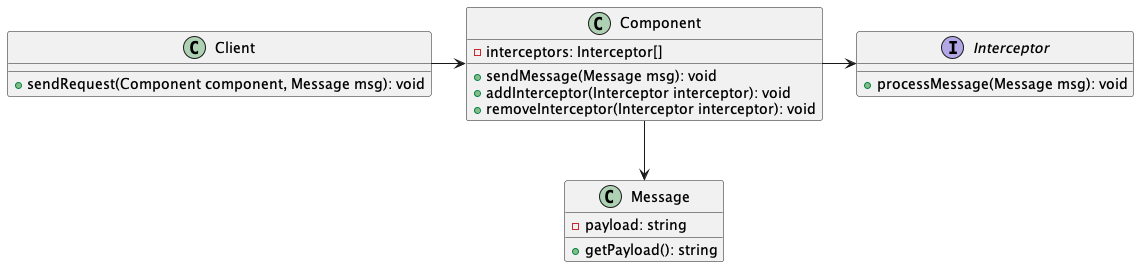
\includegraphics[width=0.99\textwidth]{fig/uml/intercept-class.png}
  \caption{Interceptor Pattern}
  \label{fig:intercept-class}
\end{figure}

Die Verwendung des Interceptor Patterns bietet mehrere Vorteile, wie z.B. die Möglichkeit, die Funktionalität einer Anwendung flexibel zu erweitern, ohne Änderungen am Quellcode der Anwendung selbst vornehmen zu müssen. Es ermöglicht auch eine effektive Steuerung der Kommunikation zwischen Komponenten und kann dazu beitragen, die Sicherheit, Leistung und Zuverlässigkeit der Anwendung zu verbessern.

\begin{figure}[!ht]
  \centering
  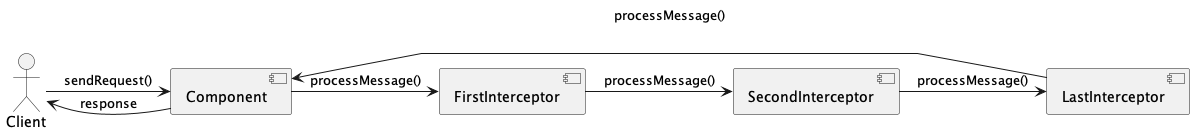
\includegraphics[width=0.99\textwidth]{fig/uml/intercept-seq.png}
  \caption{Interceptor Pattern Sequenz}
  \label{fig:intercept-seq}
\end{figure}

In dem Beispiel der Abbildung~\ref{fig:intercept-seq} besteht die Component aus einer Kette von Interceptor-Komponenten (FirstInterceptor, SecondInterceptor und LastInterceptor), die die eingehenden Nachrichten abfangen und modifizieren können. Die Client-Komponente sendet eine Nachricht an die Component, die dann durch die Kette von Interceptor-Komponenten läuft, bevor sie an die Client-Komponente zurückgesendet wird.

Das Klassendiagramm~\ref{fig:intercept-class} zeigt die verschiedenen Klassen und deren Beziehungen zueinander, während das Sequenzdiagramm zeigt, wie die verschiedenen Komponenten miteinander interagieren. In beiden Diagrammen ist die Verwendung des Interceptor Patterns deutlich zu erkennen.

Ein Beispiel für das Interceptor Pattern in einem verteilten System könnte wie folgt aussehen. Zunächst werden die Annahmen für das Beispiel getroffen. 
\begin{itemize}   
\item Es gibt eine Anwendung, die aus mehreren Komponenten besteht, die über ein Netzwerk miteinander kommunizieren.
\item Eine dieser Komponenten ist für die Ausführung von Finanztransaktionen verantwortlich.
\end{itemize}   
Darüber müssen wir uns in dem Beispiel auch klar werden über die Anforderungen an das Pattern.
\begin{itemize}   
\item Es ist erforderlich, dass alle eingehenden und ausgehenden Finanztransaktionsnachrichten überwacht werden, um die Sicherheit und Integrität der Transaktionen zu gewährleisten.
\item Es ist auch erforderlich, dass die Leistung der Finanztransaktionen überwacht wird, um sicherzustellen, dass die Anwendung reibungslos läuft.
\end{itemize}   
Nicht zu Letzt sind die Aspekte der Implementierung zu diskutieren:
\begin{itemize}   
\item Der erste Interceptor in der Kette ist für die Überprüfung der Sicherheit der Finanztransaktionsnachrichten verantwortlich. Wenn die Nachricht sicherheitsrelevant ist, wird sie an den nächsten Interceptor weitergeleitet. Wenn die Nachricht jedoch als unsicher eingestuft wird, wird sie abgelehnt.
\item Der zweite Interceptor in der Kette ist für die Überwachung der Leistung der Finanztransaktionen verantwortlich. Wenn die Nachricht eine Finanztransaktion ist, wird die Leistung der Transaktion gemessen und protokolliert.
\item Der letzte Interceptor in der Kette ist für das Senden der Finanztransaktionsnachricht an die Zielkomponente verantwortlich.
\end{itemize} 
Durch die Verwendung des Interceptor Patterns können die Finanztransaktionen sicher und effektiv überwacht werden, ohne dass Änderungen am Quellcode der Anwendung selbst vorgenommen werden müssen. Die Interceptor-Komponenten können auch problemlos hinzugefügt, entfernt oder geändert werden, um den Anforderungen der Anwendung gerecht zu werden.

\subsubsection{Fassade Pattern}
Das Fassade Pattern ist ein Strukturpattern, das in verteilten Systemen verwendet werden kann, um eine vereinfachte Schnittstelle für den Zugriff auf komplexe Subsysteme bereitzustellen. Es dient als eine Art vereinfachte Schicht, die die Interaktion zwischen Client-Code und einem komplexen Subsystem abstrahiert.

In verteilten Systemen kann das Fassade Pattern genutzt werden, um die Komplexität von Systemen zu reduzieren, indem eine einzige Schnittstelle bereitgestellt wird, die als Einstiegspunkt für den Zugriff auf das System dient. Dies kann dazu beitragen, die Komplexität des Systems für den Benutzer zu reduzieren und die Wartbarkeit des Codes zu verbessern.

Das Fassade Pattern besteht aus einer Fassadenklasse, die eine vereinfachte Schnittstelle für den Zugriff auf ein komplexes Subsystem bereitstellt. Die Fassade delegiert dann die Anfragen des Clients an das Subsystem, um die gewünschten Aktionen auszuführen. Die Fassadeklasse kapselt somit das komplexe Subsystem und stellt dem Client nur eine einfachere Schnittstelle zur Verfügung.

Ein Beispiel für die Verwendung des Fassade Patterns in verteilten Systemen könnte die Verwendung einer zentralen Authentifizierungs- und Autorisierungsschicht sein. Eine Fassadenklasse könnte erstellt werden, die als Schnittstelle für den Zugriff auf diese Schicht fungiert. Die Fassadenklasse könnte dann die Anfragen des Clients an das Authentifizierungs- und Autorisierungssystem weiterleiten, um die gewünschten Aktionen auszuführen.

\noindent\begin{minipage}{\textwidth}
\begin{lstlisting}[caption={Fassade Pattern},captionpos=b,label={lst:fassade}]
// Das komplexe Subsystem
class SubsystemA {
    public void operationA() {
        // komplexe Logik
    }
}

class SubsystemB {
    public void operationB() {
        // komplexe Logik
    }
}

// Die Fassade
class Facade {
    private SubsystemA subsystemA;
    private SubsystemB subsystemB;
    
    public Facade() {
        this.subsystemA = new SubsystemA();
        this.subsystemB = new SubsystemB();
    }
    
    // Einfache Schnittstelle fuer den Client
    public void performAction() {
        subsystemA.operationA();
        subsystemB.operationB();
    }
}

// Client Code
class Client {
    public static void main(String[] args) {
        Facade facade = new Facade();
        facade.performAction();
    }
}
\end{lstlisting}
\end{minipage}

In diesem Beispiel des Listings~\ref{lst:fassade} besteht das komplexe Subsystem aus den Klassen SubsystemA und SubsystemB, die jeweils eine komplexe Logik ausführen. Die Facade-Klasse ist die vereinfachte Schnittstelle für den Client und delegiert die Anfragen des Clients an das Subsystem, um die gewünschten Aktionen auszuführen. In diesem Fall führt die performAction()-Methode der Fassade einfach die Operationen von SubsystemA und SubsystemB aus.

Der Client-Code erstellt eine Instanz der Fassade und ruft die performAction()-Methode auf, um auf das komplexe Subsystem zuzugreifen. Die Fassade kapselt somit das komplexe Subsystem und stellt dem Client nur eine einfachere Schnittstelle zur Verfügung.




\subsubsection{Pipeline Pattern}
Das Pipeline Pattern ist ein Architekturmuster für verteilte Systeme, das es ermöglicht, komplexe Verarbeitungsprozesse aufzubauen, indem die Verarbeitung in einzelne Schritte aufgeteilt wird, die sequentiell ausgeführt werden. Jeder Schritt wird von einem spezialisierten Modul durchgeführt, das in der Lage ist, einen bestimmten Verarbeitungsschritt auszuführen. Im Pipeline Pattern gibt es drei grundlegende Komponenten:
\begin{itemize} 
\item Die Pipeline: eine Abfolge von Verarbeitungsschritten, die in einer bestimmten Reihenfolge ausgeführt werden.
\item Die Module: spezialisierte Komponenten, die für die Durchführung jedes Verarbeitungsschritts verantwortlich sind.
\item Die Daten: die Eingabe- oder Ausgabedaten, die durch die Pipeline fließen und von den Modulen verarbeitet werden.
\end{itemize} 
Ein Beispiel für das Pipeline Pattern könnte ein System sein, das große Datenmengen verarbeiten muss. Die Daten könnten in mehrere Schritte unterteilt werden, wie z.B. das Lesen von Daten aus einer Quelle, das Filtern von Daten, das Aggregieren von Daten und das Speichern von Daten in einer Datenbank. Jeder dieser Schritte wird von einem spezialisierten Modul durchgeführt, das in der Lage ist, diesen Verarbeitungsschritt effizient auszuführen.

Das Pipeline Pattern bietet eine Vielzahl von Vorteilen für verteilte Systeme, wie z.B. eine bessere Skalierbarkeit und Flexibilität bei der Entwicklung von komplexen Verarbeitungsprozessen. Es ermöglicht auch eine bessere Wiederverwendbarkeit von Modulen und eine einfachere Wartung und Fehlerbehebung. Allerdings erfordert das Pipeline Pattern auch eine sorgfältige Planung und Gestaltung der einzelnen Verarbeitungsschritte und Module, um eine optimale Leistung und Skalierbarkeit zu gewährleisten.

\subsubsection{Watchdog}
Das Watchdog Pattern ist ein bekanntes Entwurfsmuster in der Softwareentwicklung, das zur Überwachung von Ressourcen oder Prozessen in einem System verwendet wird. Es ist besonders nützlich, um potenzielle Fehler oder Störungen frühzeitig zu erkennen und entsprechende Maßnahmen zu ergreifen, um die Stabilität und Zuverlässigkeit der Anwendung zu gewährleisten.

Im Wesentlichen besteht das Watchdog Pattern aus zwei Hauptkomponenten: dem Watchdog und dem überwachten System oder Prozess. Der Watchdog ist ein unabhängiger Prozess, der den Zustand und das Verhalten des überwachten Systems kontinuierlich überprüft. Dazu verwendet der Watchdog bestimmte Prüfkriterien oder Zeitintervalle, um festzustellen, ob das überwachte System ordnungsgemäß funktioniert oder ob es Anzeichen für Fehlfunktionen gibt.

Sollte der Watchdog feststellen, dass das überwachte System nicht mehr ordnungsgemäß funktioniert, kann er entsprechende Maßnahmen ergreifen, um das Problem zu beheben. Dies kann beispielsweise das Neustarten des fehlerhaften Prozesses, das Senden einer Benachrichtigung an einen Administrator oder das Ausführen von Fallback- oder Wiederherstellungsmechanismen sein.

Das Watchdog Pattern ist in verschiedenen Anwendungsbereichen, wie zum Beispiel eingebetteten Systemen, verteilten Systemen oder auch bei der Überwachung von Softwarekomponenten, sehr nützlich. Es hilft dabei, die Systemverfügbarkeit und -stabilität zu erhöhen und die Auswirkungen von Fehlern oder Störungen zu minimieren.

Ein wichtiger Aspekt bei der Implementierung des Watchdog Patterns ist die Trennung der Verantwortlichkeiten zwischen dem Watchdog und dem überwachten System. Der Watchdog sollte so unabhängig wie möglich vom überwachten System agieren, um sicherzustellen, dass er selbst nicht von den Problemen betroffen ist, die er überwachen soll. Dies kann beispielsweise durch die Verwendung von separaten Prozessen oder Threads erreicht werden.

Insgesamt ist das Watchdog Pattern ein leistungsfähiges Entwurfsmuster, das dazu beiträgt, die Robustheit und Zuverlässigkeit von Softwaresystemen zu erhöhen. Durch die frühzeitige Erkennung und Behebung von Problemen kann es dazu beitragen, die Ausfallzeiten und die potenziellen Auswirkungen auf Benutzer und Kunden zu reduzieren.

\subsubsection{Master-Worker Pattern}
Das Master-Worker Pattern, auch bekannt als Master-Slave Pattern, ist ein grundlegendes Entwurfsmuster in der Informatik, das nicht speziell für verteilte Systeme entwickelt wurde. Es ist eine Methode zur Organisation von Systemen, bei der eine zentrale Einheit (Master) die Kontrolle über mehrere untergeordnete Einheiten (Worker) hat. Das Hauptziel dieses Musters ist es, die Arbeitslast effizient auf mehrere Prozessoren oder Knoten zu verteilen und die Skalierbarkeit und Zuverlässigkeit des Gesamtsystems zu verbessern.

In verteilten Systemen der Informatik ist das Master-Worker Pattern von großer Bedeutung, da es die folgenden Vorteile bietet:
\begin{itemize} 
\item Parallelisierung: Das Muster erlaubt die Aufteilung von Arbeitslasten auf mehrere Worker, wodurch Aufgaben parallel und somit schneller ausgeführt werden können. Dies ist besonders nützlich bei rechenintensiven Aufgaben und bei Systemen, bei denen Ressourcen effizient genutzt werden müssen.
\item Skalierbarkeit: Das Master-Worker Pattern ermöglicht es, einem System einfach neue Worker hinzuzufügen oder bestehende Worker zu entfernen, um die Systemleistung je nach Bedarf anzupassen. Dadurch kann das System auch bei wachsenden Anforderungen weiterhin effizient arbeiten.
\item Fehlertoleranz: Da das System aus mehreren unabhängigen Workern besteht, kann es bei einem Ausfall eines Workers immer noch weiterarbeiten. Der Master kann den ausgefallenen Worker ersetzen oder dessen Aufgaben auf andere Worker verteilen, um sicherzustellen, dass das System trotz des Ausfalls weiterhin funktioniert.
\item Vereinfachung der Anwendungsentwicklung: Das Master-Worker Pattern ermöglicht es den Entwicklern, ihre Anwendungen zu modularisieren, indem sie die Funktionalität auf verschiedene Worker aufteilen. Dadurch können Entwickler sich auf einzelne Teilaufgaben konzentrieren, was die Anwendungsentwicklung und -wartung vereinfacht.
\end{itemize}    

Ein Beispiel für die Verwendung des Master-Worker Patterns ist das MapReduce-Paradigma, das in verteilten Datenverarbeitungssystemen wie Hadoop verwendet wird. Der Master, auch als \enquote{Jobtracker} bezeichnet, teilt die Eingabedaten in kleinere Teile auf und weist diese den Workern, auch als \enquote{Tasktracker} bezeichnet, zur Verarbeitung zu. Die Worker führen ihre zugewiesenen Aufgaben aus und melden ihre Ergebnisse zurück an den Master, der diese dann zu einem einzigen Ergebnis zusammenführt.

\label{Woche05}
\paragraph{MapReduce-Paradigma\\\\}

Das MapReduce-Paradigma wurde erstmals von Google im Jahr 2004 eingeführt und ist seitdem zu einem grundlegenden Baustein in der Verarbeitung großer Datenmengen geworden, insbesondere im Bereich des Big Data und der Datenanalyse. MapReduce besteht aus zwei Hauptphasen: Map und Reduce.
\begin{itemize}  
\item Map-Phase: In dieser Phase werden die Eingabedaten in Key-Value-Paare aufgeteilt und anschließend parallel über die verfügbaren Knoten im Cluster verteilt. Die Map-Funktion wird auf jedem dieser Knoten ausgeführt und verarbeitet die zugeordneten Key-Value-Paare. Die Ausgabe der Map-Funktion ist eine Liste von Zwischen-Key-Value-Paaren.
\item Reduce-Phase: Die Zwischen-Key-Value-Paare aus der Map-Phase werden nach dem Schlüssel gruppiert und an die Reduce-Funktion weitergeleitet. Die Reduce-Funktion wird auf jedem Gruppenschlüssel ausgeführt und fasst die zugehörigen Werte zusammen, um die endgültigen Ergebnisse zu erzeugen.
\end{itemize}  

Ein einfaches Beispiel für das MapReduce-Paradigma ist die Wortzählung in einem Text. Angenommen, wir haben einen großen Text und möchten die Häufigkeit jedes Wortes zählen. Hier ist, wie wir dies mit MapReduce erreichen können:
\begin{itemize} 
\item Map-Phase: Zuerst wird der Text in kleinere Abschnitte aufgeteilt und auf verschiedene Knoten im Cluster verteilt. Die Map-Funktion wird auf jedem Knoten ausgeführt, um jedes Wort in den Abschnitten zu verarbeiten.

Die Map-Funktion liest die Wörter in ihrem zugewiesenen Abschnitt und erstellt ein Key-Value-Paar für jedes Wort, wobei der Schlüssel das Wort selbst ist und der Wert 1. Wenn das Wort \enquote{Hallo} beispielsweise dreimal im Abschnitt erscheint, gibt die Map-Funktion folgende Key-Value-Paare aus:\\\\

\noindent\begin{minipage}{\textwidth}
\begin{lstlisting}[caption={Ausgabe},captionpos=b,label={lst:mapI}]
("Hallo", 1)
("Hallo", 1)
("Hallo", 1)
\end{lstlisting}
\end{minipage}

\item Reduce-Phase: Nachdem die Map-Phase abgeschlossen ist, werden die Key-Value-Paare nach dem Schlüssel (Wort) gruppiert und an die Reduce-Funktion gesendet. In diesem Fall hätten wir eine Gruppe für das Wort \enquote{Hallo} mit den Werten [1, 1, 1].

Die Reduce-Funktion summiert die Werte für jedes Wort, um die endgültige Häufigkeit zu erhalten. Für das Wort \enquote{Hallo} würde die Reduce-Funktion die Werte addieren (1 + 1 + 1) und das endgültige Key-Value-Paar ausgeben: \\\\

\noindent\begin{minipage}{\textwidth}
\begin{lstlisting}[caption={Ausgabe},captionpos=b,label={lst:mapII}]
("Hallo", 3)
\end{lstlisting}
\end{minipage}
\end{itemize}  

Nachdem alle Reduce-Funktionen ausgeführt wurden, haben wir eine Liste von Key-Value-Paaren, die die Häufigkeit jedes Wortes im gesamten Text angeben.

Dieses Beispiel veranschaulicht die grundlegenden Schritte des MapReduce-Paradigmas. In der Praxis würde ein MapReduce-Framework wie Apache Hadoop diese Phasen automatisch auf einem Cluster von Computern ausführen und die Verarbeitung von großen Datenmengen ermöglichen.


\subsection{Beispielarchitekturen}
Die Remote Procedure Call (RPC) Architektur und die Peer-to-Peer (P2P) Architektur sind zwei grundlegend unterschiedliche Ansätze zur Entwicklung verteilter Systeme, die jeweils ihre eigenen Stärken und Schwächen aufweisen. Beide Architekturen bieten Lösungen für verschiedene Anwendungsfälle und Probleme, die in verteilter Systementwicklung auftreten. Durch das Vergleichen dieser beiden Beispielarchitekturen können wir ein besseres Verständnis der verschiedenen Aspekte und Herausforderungen bei der Entwicklung verteilter Systeme gewinnen.
\subsubsection{Remote Procedure Call}

Die Remote Procedure Call (RPC) Architektur ist ein Kommunikationsmodell, das es ermöglicht, Prozeduraufrufe zwischen Prozessen auf unterschiedlichen Systemen oder Maschinen durchzuführen. Die Idee hinter RPC besteht darin, entfernte Funktionen oder Methoden so einfach aufrufen zu können, als wären sie lokale Funktionen innerhalb des aufrufenden Programms.
\\\\
Aufbau einer RPC-Architektur:
\begin{itemize} 
\item \textbf{Client}: Der Client ist der Prozess oder die Anwendung, die den entfernten Prozeduraufruf initiiert. Der Client stellt eine Anfrage an den Server, um eine bestimmte Funktion auszuführen, und wartet auf die Antwort.
\item \textbf{Client Stub}: Der Client Stub ist eine lokale Repräsentation der entfernten Prozedur auf der Clientseite. Er ist dafür verantwortlich, die Anfrage des Clients in ein geeignetes Format umzuwandeln, das vom Server verstanden werden kann. Dieser Vorgang wird als \enquote{Marshalling} bezeichnet.
\item \textbf{Kommunikationsprotokoll}: Ein Kommunikationsprotokoll wird verwendet, um die Anfrage und die Antwort zwischen Client und Server zu übertragen. Dies kann beispielsweise ein TCP/IP- oder UDP-Protokoll sein, je nach den Anforderungen an Zuverlässigkeit, Geschwindigkeit und Latenz.
\item \textbf{Server}: Der Server ist der Prozess oder die Anwendung, die die angeforderte Funktion oder Methode bereitstellt. Der Server empfängt die Anfrage vom Client, führt die entsprechende Prozedur aus und sendet die Antwort zurück.
\item \textbf{Server Stub}: Der Server Stub empfängt die Anfrage vom Client, wandelt sie in ein für die Serverumgebung geeignetes Format um (\enquote{Unmarshalling}) und ruft die gewünschte Funktion auf. Anschließend werden die Ergebnisse wieder \enquote{gemarshalled} und an den Client gesendet.
\end{itemize}     
Im Folgenden wird der grundsätzliche Ablauf in einer RPC Architektur beschrieben, welcher noch verfeinert werden sollte, aber bereits die grundlegende Idee transportiert. 
\begin{enumerate} 
\item Der Client ruft die entfernte Prozedur über den Client Stub auf, als wäre es eine lokale Funktion.
\item Der Client Stub wandelt die Parameter der Anfrage in ein standardisiertes Format um (Marshalling) und sendet die Anfrage über das Kommunikationsprotokoll an den Server.
\item Der Server Stub empfängt die Anfrage, demarshalled die Parameter und ruft die entsprechende Funktion auf dem Server auf.
\item Die Funktion wird auf dem Server ausgeführt, und das Ergebnis wird an den Server Stub zurückgegeben.
\item Der Server Stub marshallt das Ergebnis und sendet es über das Kommunikationsprotokoll an den Client Stub zurück.
\item Der Client Stub empfängt die Antwort, demarshalled das Ergebnis und gibt es an den Client zurück.
\end{enumerate}
In einer RPC-Architektur kann die Kommunikation sowohl synchron als auch asynchron erfolgen. Bei synchroner Kommunikation wartet der Client auf die Antwort vom Server, bevor er weitere Aktionen ausführt. Dies kann zu Wartezeiten führen, insbesondere bei langsamen Netzwerkverbindungen oder komplexen Anfragen. 

Bei asynchroner Kommunikation sendet der Client die Anfrage und führt sofort weitere Aufgaben aus, ohne auf die Antwort zu warten. Die Antwort wird in der Regel über einen Callback-Mechanismus oder ein Event-System verarbeitet, sobald sie verfügbar ist.
\\\\
Die RPC-Architektur ist in verschiedenen Anwendungen und Umgebungen weit verbreitet, wie z.B. bei klassischen Client-Server-Anwendungen oder Microservices. Sie bietet eine abstrakte und einfach zu verwendende Schnittstelle für die Kommunikation zwischen Prozessen auf verschiedenen Systemen, ohne dass sich der Entwickler um die Details der Netzwerkkommunikation kümmern muss.
\\\\
Das Diagramm in der Abbildung~\ref{fig:simple-rpc} zeigt einen ersten naiven Entwurf einer RPC Schichtenarchitektur. In diesem Ansatz existiert eine Schicht \enquote{Application}, welche die Schicht der Middleware nutzt, welche wiederum die Ressourcen - beispielhaft des Betriebssystems - nutzt, um die Kommunikation mittels Netzwerkprotokolle zu realisieren. \\\\

\begin{figure}[!ht]
  \centering
  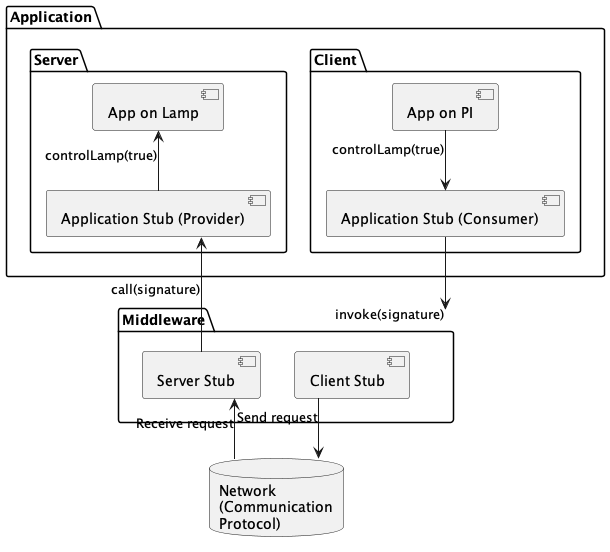
\includegraphics[width=0.95\textwidth]{fig/uml/rpc-simple.png}
  \caption{Erster Ansatz einer RPC Architektur}
  \label{fig:simple-rpc}
\end{figure}

Interessant ist die Einbringung einer zusätzlichen Schicht in der Applikation, die als \textbf{Application Stub} bezeichnet ist. Die Idee des Application-Stubs (auch als \enquote{Applikations-Stub} oder \enquote{App-Stub} bezeichnet) wurde von Andrew S. Tanenbaum entwickelt, um die Kommunikation und Interaktion zwischen Anwendungen und Middleware in verteilten Systemen zu erleichtern. Der Application-Stub ist eine Schnittstelle, die als Vermittler zwischen der Anwendung und der Middleware fungiert, um die Kommunikation und Zusammenarbeit zwischen diesen beiden Ebenen zu ermöglichen. Dies ist ein klassisches drei-schichtiges Modell.
\\\\
Die Umsetzung des Application-Stubs basiert auf der Trennung der Anwendungslogik von der Middleware-Kommunikationslogik. Dies wird erreicht, indem der Stub die Anwendungslogik von den Netzwerkdetails, wie z.B. den Marshalling/Unmarshalling von Daten, dem Verbindungsaufbau und dem Senden/Empfangen von Nachrichten, entkoppelt.
In einfache Worten gesprochen, bindet das Application-Stub die Applikation mit der Middleware, ohne das die Applikation Kenntnis von der Middleware hat und die Middleware keine Kenntnis über die Applikation.
\\\\
Um den Application-Stub in einer verteilten Umgebung zu nutzen, sind folgende Schritte erforderlich:
\begin{itemize} 
\item Entwurf einer Schnittstellenbeschreibung: Zunächst wird eine Schnittstellenbeschreibung erstellt, die die Funktionen und Methoden definiert, die von der Anwendung und der Middleware bereitgestellt werden sollen. Diese Schnittstellenbeschreibung kann in einer \textbf{Interface Definition Language }(IDL) oder einer ähnlichen Sprache definiert werden.
\item Erstellung des Application-Stubs: Basierend auf der Schnittstellenbeschreibung wird ein Application-Stub generiert oder manuell erstellt. Dieser Stub enthält Code, der die Kommunikation zwischen der Anwendung und der Middleware verwaltet. Es kann für verschiedene Programmiersprachen und Plattformen erstellt werden, um die Interoperabilität zu gewährleisten.
\item Integration des Application-Stubs in die Anwendung: Der generierte oder erstellte Application-Stub wird in die Anwendung integriert, indem er die definierten Funktionen und Methoden für die Kommunikation mit der Middleware implementiert. Die Anwendung ruft die Funktionen und Methoden des Stubs auf, als wären sie lokale Funktionen oder Methoden, ohne sich um die zugrunde liegenden Netzwerkdetails kümmern zu müssen. Das Factory Pattern kann hier eine Lösung sein, die Wahl zu implementieren.
\item Anpassung der Middleware: Die Middleware muss in der Lage sein, die Anfragen des Application-Stubs zu verarbeiten und entsprechend zu reagieren. Dies kann durch die Implementierung von Server-Stubs und der entsprechenden Kommunikationslogik erreicht werden.
\item Kommunikation zwischen Anwendung und Middleware: Durch die Verwendung des Application-Stubs kann die Anwendung nun nahtlos mit der Middleware kommunizieren, ohne sich um die Details der Netzwerkkommunikation kümmern zu müssen. Die Middleware empfängt die Anfragen, verarbeitet sie und sendet die Ergebnisse zurück an die Anwendung über den Application-Stub.
\end{itemize} 
Der Application-Stub ermöglicht nach Tanenbaum eine effiziente Kommunikation und Zusammenarbeit zwischen Anwendungen und Middleware in verteilten Systemen. Durch die Entkopplung der Anwendungslogik von der Kommunikationslogik können Entwickler sich auf die wesentlichen Aspekte der Anwendung konzentrieren, während die Middleware die Netzwerkkommunikation und andere Details verwaltet.
\\\\
Hier ist ein einfaches Beispiel in Java, das die Idee des Application-Stubs und das Factory-Pattern verwendet, um eine Anwendung mit Middleware zu verbinden. In diesem Beispiel simulieren wir eine einfache Lampe und ihre Steuerung.
Zuerst erstellen wir eine Lamp-Schnittstelle, die als Middleware fungiert:\\\\
\noindent\begin{minipage}{\textwidth}
\begin{lstlisting}[caption={RPC Interface},captionpos=b,label={lst:rpc-interface}]
public interface Lamp {
    void controlLamp(Boolean b);
}
\end{lstlisting}
\end{minipage}
Als nächstes erstellen wir eine Implementierung der Lamp-Schnittstelle auf dem Server-Anteil des Applikationscodes:\\\\

\noindent\begin{minipage}{\textwidth}
\begin{lstlisting}[caption={RPC Remote Implementation},captionpos=b,label={lst:rpc-remote}]
public class LampRemote implements Lamp {
    @Override
    public void controlLamp(boolean b){
    	List<Boolean> list = new ArrayList<Boolean>(); 
        Collections.addAll(list, b);
        Middleware.invoke("controlLamp", list);
    }
}
\end{lstlisting}
\end{minipage}
Nun erstellen wir eine Factory-Klasse, die als Application-Stub fungiert:\\\\
\noindent\begin{minipage}{\textwidth}
\begin{lstlisting}[caption={Application Stub mit Factory Pattern},captionpos=b,label={lst:rpc-factory}]
public class LampFactory {
    public static Lamp createLamp() {
        // Hier koennte die Middleware-Verbindung hergestellt werden.
        // In diesem Beispiel verwenden wir eine einfache lokale Implementierung.
        return new LampRemote();
    }
}
\end{lstlisting}
\end{minipage}
Schließlich erstellen wir eine Anwendungsklasse, die die Lamp-Schnittstelle verwendet:\\\\
\noindent\begin{minipage}{\textwidth}
\begin{lstlisting}[caption={Controller ruft Middleware},captionpos=b,label={lst:rpc-controller}]
public class LampController {
	public static void main(String[] args) {
        // Erstelle eine Lampe ueber die Factory-Methode (Application-Stub)
        Lamp lamp = LampFactory.createLamp();

        // Verwende die Lampe in der Anwendung
        lamp.controlLamp(true);
    }
}
\end{lstlisting}
\end{minipage}
In diesem Beispiel wurde eine Lamp-Schnittstelle erstellt, die als Middleware fungiert, um eine Lampe aus der Entfernung (über Netzwerk) zu steuern. Die LampFactory-Klasse dient als Application-Stub, der die Erstellung und Verbindung zur Middleware verwaltet. Die Lamp Controller-Anwendung verwendet die Lamp-Schnittstelle über die Factory-Methode, um die Lampe ein- und auszuschalten.
\\\\
In einer realen Anwendung könnte die LampFactory-Klasse die Verbindung zu einer tatsächlichen Middleware herstellen, anstatt einfach eine lokale Implementierung zu erstellen. Natürlich ist die Annahme einer Objektmenge nur aus dem Datentyp Boolean naiv, zeigt aber die Funktionsweise ausreichend auf. Die Anwendung selbst muss sich jedoch nicht um diese Details kümmern, da der Application-Stub diese Verantwortung übernimmt.
\\\\
Diese zunächst einfache und naive Darstellung ist als Möglichkeit gedacht, um zunächst einen Überblick zu schaffen. Natürlich müssen hier verschiedene Aspekte verfeinert und für das bessere Verständnis nochmal diskutiert werden. Hier wird auf das Praktikum verwiesen.
\\\\
Als erstes muss man aber bereits festhalten, dass aus der naiven Ansicht der statischen Komponentensicht häufig ein Verhalten abgeleitet wird, welches aber auf einer missverstandenen Interpretation der Architektur zurückzuführen ist, weniger auf ein noch nicht eingeführtes Verhalten.  
\\\\
Ist die Beschreibung des Verhaltens in der Architektur das Ziel, muss nochmals auf die Nutzung des Schichtenmodells hingewiesen werden. Jede Schicht kapselt die Sequenzen nach der zugeordneten Verantwortlichkeit.
Somit beschreiben die Sequenzen in der Applikationsschicht die der Applikation und die Sequenzen der Middleware die der Middleware. Was nicht geschehen sollte, ist eine Vermischung beider Schichten. So wäre eine gültige Sequenz der Applikation beschrieben in Diagramm~\ref{fig:rpc-app-seq-rpc} und eine der Middleware im Diagramm~\ref{fig:rpc-middleware-seq-rpc}. An der Sequenz in der Applikation selbst sollte man nicht ohne weiteres erkennen, dass es sich um einen entfernen Funktionsaufruf handelt. Diese Aufgabe wird von der Middleware übernommen.
\\\\
Es ist wichtig zu verstehen, dass die Sequenz der Applikation aus einer spezifischen Verarbeitung des Anwendungsfalls getrieben ist, wohingegen die Sequenz der Middleware eine generische Umsetzung repräsentiert, die von jeglichem Aufruf aus der Applikation heraus genutzt werden kann, solange sie die gleichen Charaktereigenschaften teilen. So kann man naiv die Beziehung zwischen einem entfernten Funktionsaufruf und der Middleware auch als eine 0:n- Beziehung beschreiben, wobei die Middleware  in diesem Fall eine generische Funktion für einen synchronen Funktionsaufruf repräsentiert. \\\\


 \begin{figure}[!ht]
  \centering
  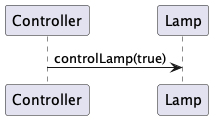
\includegraphics[width=0.30\textwidth]{fig/uml/rpc-app-seq.png}
  \caption{Beispielsequenz der App in der RPC Architektur}
  \label{fig:rpc-app-seq-rpc}
\end{figure}


 \begin{figure}[!ht]
  \centering
  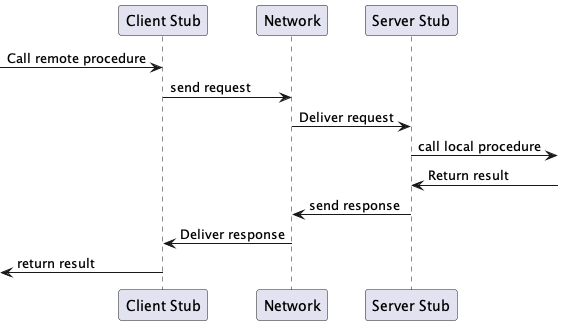
\includegraphics[width=0.65\textwidth]{fig/uml/rpc-middleware-seq.png}
  \caption{Beispielsequenz der Middleware in der RPC Architektur}
  \label{fig:rpc-middleware-seq-rpc}
\end{figure}

Um die Middleware möglichst transparent und wiederverwendbar zu gestalten, soll der Marshalling-Prozess genauer betrachtet werden, der im Client-Stub und Server-Stub eine besondere Rolle spielt, bevor die Nachrichten für den entfernten Funktionsaufruf versendet werden. 
\paragraph{Marshalling\\\\}
Der Marshalling-Prozess und die Serialisierung sind Begriffe, die oft im Zusammenhang mit der Remote Procedure Call (RPC) Architektur verwendet werden. Beide Prozesse sind zwar miteinander verknüpft, es gibt jedoch grundlegende Unterschiede zwischen ihnen.
\\\\
Der Marshalling-Prozess ist ein Verfahren, bei dem Daten und Parameter in einer Form gewandelt werden, die über das Netzwerk gesendet und auf der anderen Seite wieder zusammengesetzt werden kann. Kurz: aus einem Funktionsaufruf wird eine Nachricht generiert. Dieser Prozess ist in der RPC-Architektur besonders wichtig, da hierdurch entfernte Prozeduraufrufe zwischen verschiedenen Systemen mit unterschiedlichen Datenformaten, Speicherlayouts oder sogar Programmiersprachen umgesetzt werden können.
\\\\
Der Marshalling-Prozess besteht aus mehreren Schritten:
\begin{itemize} 
\item Umwandlung der Daten und Parameter in ein plattformunabhängiges Format, oft in Form von Byte-Arrays.
\item Anfügen von Metadaten, wie zum Beispiel Typinformationen, um den Empfänger darüber zu informieren, wie die Daten wiederhergestellt werden können.
\item Zusammenpacken (Packing) der Daten und Metadaten in einer Nachricht, die über das Netzwerk gesendet werden kann.
\end{itemize} 

Die Serialisierung ist der Prozess der Umwandlung eines Objekts oder einer Datenstruktur in eine lineare, sequenzielle Darstellung, die zum Speichern oder Übertragen über ein Netzwerk verwendet werden kann. Serialisierung ist ein wichtiger Teil des Marshalling-Prozesses, da sie die Daten in eine übertragbare Form konvertiert. Sie ermöglicht es, den Zustand eines Objekts oder einer Datenstruktur zu erhalten, sodass es auf der Empfängerseite wiederhergestellt und verwendet werden kann. Unterschiede zwischen Marshalling und Serialisierung:
\begin{itemize} 
\item Anwendungsbereich: Serialisierung ist ein generischer Prozess, der nicht nur in der RPC-Architektur, sondern auch in anderen Anwendungen wie der persistenten Speicherung von Objekten und der Interprozesskommunikation verwendet wird. Marshalling ist spezifisch für die RPC-Architektur und bezieht sich auf das Vorbereiten von Daten und Parametern für entfernte Prozeduraufrufe.
\item Metadaten: Marshalling beinhaltet das Hinzufügen von Metadaten, die zur Interpretation und Rekonstruktion der übertragenen Daten auf der Empfängerseite erforderlich sind. Bei der Serialisierung werden hauptsächlich die Daten selbst in eine sequenzielle Darstellung umgewandelt, ohne notwendigerweise zusätzliche Metadaten hinzuzufügen.
\end{itemize} 
Im Weiteren soll ein Beispiel für einen Marshalling-Prozess ausgearbeitet werden. Angenommen, es gibt zwei Systeme A und B, die unterschiedliche Programmiersprachen und Datenformate verwenden. System A möchte eine Funktion auf System B aufrufen, die zwei Parameter akzeptiert: einen String und einen Integer. Der Marshalling-Prozess auf System A würde wie folgt aussehen:
\begin{itemize} 
\item Konvertierung der Parameter (z.B. String und Integer) in ein plattformunabhängiges Format, z. B. Byte-Arrays.
\item Hinzufügen von Metadaten, wie Typinformationen, zur Identifizierung der Parameter auf der Empfängerseite.
\item Zusammenpacken der Byte-Arrays und Metadaten in einer Nachricht, die über das Netzwerk gesendet werden kann
\end{itemize} 

Das Ziel, den Marshalling Process möglich generisch zu gestallten, ist in dem Prinzip \enquote{Copy in, Copy out} zusammengefasst. Der Begriff \enquote{Copy in, Copy out} (auch als \enquote{Call by Value-Result} bezeichnet) ist eine Semantik zur Übergabe von Parametern bei entfernten Prozeduraufrufen (RPCs) oder in Programmiersprachen. Es beschreibt die Art und Weise, wie Daten und Parameter zwischen dem aufrufenden und dem aufgerufenen System übertragen werden. Hier ist das grundlegende Prinzip von \enquote{Copy in, Copy out}:
\begin{itemize} 
\item \textbf{Copy in}: Beim Aufruf einer entfernten Funktion kopiert das aufrufende System die Werte der Parameter in eine Nachricht, die an das aufgerufene System gesendet wird. Dieser Schritt beinhaltet den Marshalling-Prozess, bei dem die Parameter in ein plattformunabhängiges Format konvertiert und Metadaten hinzugefügt werden.
\item \textbf{Copy out}: Nachdem die entfernte Funktion auf dem aufgerufenen System ausgeführt wurde, werden die Ergebnisse (Rückgabewerte oder geänderte Parameter) zurück zum aufrufenden System gesendet. Der Rückgabewert und die geänderten Parameter durchlaufen den Marshalling-Prozess erneut, um sie in eine übertragbare Form zu bringen. Anschließend kopiert das aufrufende System die empfangenen Daten in die ursprünglichen Variablen oder Speicherbereiche.
\end{itemize} 
\enquote{Copy in, Copy out} bietet einige Vorteile: Es vermeidet die direkte Manipulation von Speicheradressen zwischen unterschiedlichen Systemen, was bei verteilten Systemen mit unterschiedlichen Speicherlayouts und Adressräumen problematisch sein kann. Weiterhin stellt es sicher, dass das aufgerufene System nur auf Kopien der übergebenen Daten arbeitet, wodurch Seiteneffekte und unerwartete Änderungen der Daten auf dem aufrufenden System vermieden werden. Zuletzt erlaubt es die Verwendung verschiedener Programmiersprachen und Datenformate auf dem aufrufenden und aufgerufenen System, da die Daten beim Marshalling in ein plattformunabhängiges Format konvertiert werden.

Ein Nachteil von \enquote{Copy in, Copy out} ist jedoch der zusätzliche Overhead, der durch das Kopieren und Marshalling/Unmarshalling der Daten entsteht. Dies kann die Leistung und Effizienz des entfernten Prozeduraufrufs beeinträchtigen, insbesondere bei großen Datenmengen oder komplexen Datenstrukturen. In solchen Fällen können andere Parameterübergabemechanismen, wie beispielsweise \enquote{Call by Reference}, in Betracht gezogen werden, bei denen nur die Speicheradressen der Daten übertragen werden und somit der Overhead reduziert wird. 

Allerdings bringt dies auch zusätzliche Herausforderungen und Risiken mit sich, wie zum Beispiel die Notwendigkeit, die unterschiedlichen Adressräume der beteiligten Systeme zu verwalten, und das Risiko unerwarteter Seiteneffekte, wenn das aufgerufene System direkt auf den Speicher des aufrufenden Systems zugreift.
\\\\
Um den Overhead bei der Verwendung von \enquote{Copy in, Copy out} zu minimieren, können verschiedene Optimierungen angewendet werden, wie zum Beispiel:

\begin{itemize} 
\item Datenkompression: Durch die Komprimierung der Daten während des Mar-shalling-Prozesses kann die Menge der übertragenen Daten reduziert werden, was zu einer schnelleren Übertragung und geringeren Netzwerkbelastung führt.
\item Verwendung effizienter Serialisierungsformate: Einige Serialisierungsformate, wie beispielsweise Protocol Buffers oder MessagePack, sind darauf ausgelegt, Daten effizienter und kompakter zu übertragen als textbasierte Formate wie JSON oder XML.
\item Selektive Übertragung: In einigen Fällen ist es möglich, nur die notwendigen Teile einer Datenstruktur oder eines Objekts zu übertragen, anstatt das gesamte Objekt zu kopieren und zu übertragen. Dies kann den Overhead der Parameterübergabe reduzieren.
\end{itemize} 

Bei der Verwendung von \enquote{Copy in, Copy out} in der RPC-Architektur ist es wichtig, die Datentypen der Parameter und Rückgabewerte korrekt zu bestimmen, um eine erfolgreiche Kommunikation zwischen dem aufrufenden und dem aufgerufenen System zu gewährleisten. So können Prozesse automatisiert werden, um die Codeanteile in einer RPC-Middleware zu bestimmen. Diese automatisierte Code-Generierung kann in folgende Schritte durchgeführt werden:
\begin{itemize} 
\item Definieren der Schnittstellen und Datenstrukturen, die in den entfernten Prozeduraufrufen verwendet werden. Dies geschieht mittels einer Interface Definition Language (IDL). Die IDL beschreibt die Signatur der entfernten Funktionen, einschließlich der Datentypen der Parameter und Rückgabewerte
\item Generieren des Stub- und Skeleton-Codes aus der IDL-Definition. Die meisten RPC-Middleware-Tools bieten Code-Generatoren an, die aus der IDL-Definition automatisch Stub- und Skeleton-Code für verschiedene Programmiersprachen erstellen. Der Stub-Code dient als Proxy für den Aufrufer, während der Skeleton-Code die Implementierung der entfernten Funktion auf dem aufgerufenen System kapselt. Beide Teile des Codes enthalten die notwendigen Informationen über die Datentypen für das Marshalling und Unmarshalling der Daten.
\item Implementierung der entfernten Funktionen auf dem aufgerufenen System unter Verwendung des generierten Skeleton-Codes. Dies stellt sicher, dass die Implementierung der Funktionen mit den in der IDL-Definition angegebenen Datentypen übereinstimmt.
\item  Verwendung des generierten Stub-Codes auf dem aufrufenden System, um entfernte Prozeduraufrufe durchzuführen. Der Stub-Code stellt sicher, dass die Parameter und Rückgabewerte korrekt gemarshalled und unmarshalled werden, basierend auf den in der IDL-Definition festgelegten Datentypen.
\end{itemize} 

\paragraph{Interface Definition Language (IDL)\\\\}

Zentrale Komponente ist die  Interface Definition Language (IDL). Eine Interface Definition Language ist eine formale Beschreibungssprache, die verwendet wird, um Schnittstellen zwischen Softwarekomponenten und Diensten in einer standardisierten und plattformunabhängigen Weise zu definieren. Die Verwendung einer IDL in Verbindung mit einem Code-Generator bietet mehrere Vorteile für die automatische Erstellung von Remote Procedure Call Lösungen.
\\\\
Ein Code-Generator für Interface Definition Language ist ein Software-Tool, das automatisch Code in einer oder mehreren Programmiersprachen auf der Grundlage einer IDL-Definition erstellt. Der Prozess der Codegenerierung aus einer IDL umfasst mehrere Schritte:
\begin{itemize} 
\item Analyse der IDL-Datei: Der Code-Generator liest und analysiert die IDL-Datei, die die Schnittstellendefinitionen, Funktionen, Datenstrukturen und Datentypen enthält, die für die Kommunikation zwischen den verschiedenen Komponenten eines verteilten Systems benötigt werden.
\item Parsen der IDL-Datei: Der Code-Generator verwendet einen Parser, um die IDL-Datei in einen abstrakten Syntaxbaum (AST) oder ein ähnliches internes Format zu zerlegen, dass leichter für die Codegenerierung verwendet werden kann.
\item Code-Generierung: Basierend auf dem internen Format erstellt der Code-Generator automatisch den notwendigen Client- und Server-Code für die Kommunikation über das verteilte System. Dies kann Stub- und Skeleton-Code für verschiedene Programmiersprachen umfassen, die für den Remote Procedure Call verwendet werden.
\item Sprachspezifische Anpassungen: Der Code-Generator berücksichtigt die Besonderheiten der jeweiligen Zielsprache, um sicherzustellen, dass der generierte Code den Konventionen und Syntaxanforderungen dieser Sprache entspricht. Dies umfasst die Anpassung von Datentypen, Namenskonventionen und anderen sprachspezifischen Details.
\item Code-Ausgabe: Schließlich gibt der Code-Generator den erstellten Code als Dateien aus, die in das Zielsystem integriert werden können. Dies ermöglicht Entwicklern, die generierten Stubs und Skeletons in ihrem Projekt zu verwenden, um die definierten Schnittstellen über RPC aufzurufen oder bereitzustellen.
\end{itemize} 

Aus diesen Schritten soll nun ein Beispiel abgeleitet werden, welches auch den manuellen Aufbau einer Lösung beschreibt. Angenommen, es gibt ein verteiltes System, in dem ein Client eine entfernte Funktion \enquote{add} aufrufen möchte, die zwei Integer-Parameter akzeptiert und einen Integer-Wert zurückgibt.

Zunächst wird eine Schnittstelle der entfernten Funktion in einer IDL definiert. \\\\
\noindent\begin{minipage}{\textwidth}
\begin{lstlisting}[caption={IDL Example},captionpos=b,label={lst:idl-example}]
interface MathService {
  int add(in int a, in int b);
}
\end{lstlisting}
\end{minipage}
Diese IDL-Definition beschreibt eine Schnittstelle namens \enquote{MathService} mit einer Funktion \enquote{add}, die zwei Integer-Parameter (\enquote{a} und \enquote{b}) akzeptiert und einen Integer-Wert zurückgibt.
\\\\
Aus diesen Informationen kann ein  Stub- und Skeleton-Code generiert werden. Abhängig von der verwendeten RPC-Middleware und Programmiersprache erhalten Sie möglicherweise Klassen oder Module, die die \enquote{MathService}-Schnittstelle implementieren und die notwendigen Informationen über die Datentypen enthalten.
\\\\
Danach ist die \enquote{add}-Funktion auf dem aufgerufenen System unter Verwendung des generierten Skeleton-Codes zu implementieren. So könnte eine Implementierung aussehen:\\\\
\noindent\begin{minipage}{\textwidth}
\begin{lstlisting}[caption={RPC IDL Service Impl},captionpos=b,label={lst:idl-impl}]
class MathServiceImpl(MathService):
    def add(self, a, b):
        return a + b
\end{lstlisting}
\end{minipage}
Nun kann der generierte Stub-Code auf dem aufrufenden System genutzt werden, um die \enquote{add}-Funktion über einen RPC-Aufruf aufzurufen.\\\\
\noindent\begin{minipage}{\textwidth}
\begin{lstlisting}[caption={RPC IDL Service Impl},captionpos=b,label={lst:idl-impl-service}]
math math_service_client = MathServiceStub(server_address)
result = math_service_client.add(5, 7)
print("Result of 5 + 7:", result)
\end{lstlisting}
\end{minipage}
In diesem Beispiel erstellen wir eine Instanz des MathServiceStub, der als Client für den entfernten MathService fungiert. Wir rufen die add-Funktion über den Stub auf und übergeben die Integer-Parameter 5 und 7. Der Stub kümmert sich um das Marshalling der Daten und das Senden der Anfrage an den entfernten Server. Der entfernte Server führt die Funktion add aus und sendet das Ergebnis (12) zurück zum Client. Der Stub verwaltet das Unmarshalling der Daten, und der Client erhält das korrekte Ergebnis.

Durch die korrekte Bestimmung der Datentypen und die Verwendung von IDL, Stub und Skeleton wird sichergestellt, dass die \enquote{Copy in, Copy out}-Semantik korrekt angewendet wird und die Kommunikation zwischen dem aufrufenden und dem aufgerufenen System erfolgreich ist. Zudem kann man sich durch gute Code Generatoren viel Arbeit ersparen. 

RPC-Lösungen wie XML-RPC und gRPC arbeiten auch nach dem \enquote{Copy in, Copy out}-Prinzip und nutzen die Marshalling/Unmarshalling-Techniken, um Daten zwischen den aufrufenden und aufgerufenen Systemen zu übertragen. 

XML-RPC ist eine RPC-Technik, die XML für die Kodierung von Daten und HTTP für die Datenübertragung verwendet. In diesem Beispiel implementieren wir einen einfachen Additionsdienst:\\\\

\noindent\begin{minipage}{\textwidth}
\begin{lstlisting}[caption={XML-RPC in Python},captionpos=b,label={lst:xmp-rpc-python}]
from xmlrpc.server import SimpleXMLRPCServer

def add(a, b):
    return a + b

server = SimpleXMLRPCServer(("localhost", 8080))
server.register_function(add, "add")
server.serve_forever()
\end{lstlisting}
\end{minipage}

In diesem Beispiel ist die \enquote{add}-Funktion auf dem Server registriert. Der Client verwendet einen Proxy, um die entfernte Funktion aufzurufen. Die Parameter (5 und 7) werden automatisch in XML kodiert (gemarshalled), und die Anfrage wird über HTTP an den Server gesendet. Der Server führt die Funktion aus und sendet das Ergebnis (12) zurück, das wiederum vom Client automatisch aus XML dekodiert (unmarshalled) wird.

Als alternative zu XML-RPC kann auch gRPC betrachtet werden. gRPC ist eine moderne, leistungsfähige RPC-Implementierung, die auf Protocol Buffers für die Datenkodierung und HTTP/2 für die Datenübertragung basiert. In diesem Beispiel implementieren wir denselben Additionsdienst wie im XML-RPC-Beispiel:

Zuerst definieren wir die Schnittstelle in einer Protocol Buffers IDL-Datei: \\\\

\noindent\begin{minipage}{\textwidth}
\begin{lstlisting}[caption={gRPC IDL},captionpos=b,label={lst:grpc-idl}]
syntax = "proto3";

service MathService {
  rpc Add(AddRequest) returns (AddResponse);
}

message AddRequest {
  int32 a = 1;
  int32 b = 2;
}

message AddResponse {
  int32 result = 1;
}
\end{lstlisting}
\end{minipage}

Weiter braucht es noch eine Implementierung der serverseitigen Funktion:\\\\

\noindent\begin{minipage}{\textwidth}
\begin{lstlisting}[caption={gRPC Server Python},captionpos=b,label={lst:grpc-server}]
import grpc
from concurrent import futures
import math_service_pb2
import math_service_pb2_grpc

class MathServiceImpl(math_service_pb2_grpc.MathServiceServicer):
    def Add(self, request, context):
        return math_service_pb2.AddResponse(result=request.a + request.b)

server = grpc.server(futures.ThreadPoolExecutor(max_workers=10))
math_service_pb2_grpc.add_MathServiceServicer_to_server(MathServiceImpl(), server)
server.add_insecure_port("[::]:8080")
server.start()
server.wait_for_termination()
\end{lstlisting}
\end{minipage}

\noindent\begin{minipage}{\textwidth}
\begin{lstlisting}[caption={gRPC Client Python},captionpos=b,label={lst:grpc-client}]
import grpc
import math_service_pb2
import math_service_pb2_grpc

channel = grpc.insecure_channel("localhost:8080")
stub = math_service_pb2_grpc.MathServiceStub(channel)
request = math_service_pb2.AddRequest(a=5, b=7)
response = stub.Add(request)
print("Result of 5 + 7:", response.result)
\end{lstlisting}
\end{minipage}
In diesem gRPC-Beispiel wird die Schnittstelle in einer Protocol Buffers IDL-Datei definiert. Der Server implementiert die Add-Funktion und registriert sie im gRPC-Server. Der Client erstellt einen Stub, um die entfernte Funktion aufzurufen. Die Anfrage- und Antwortdaten werden automatisch in Protocol Buffers kodiert (gemarshalled) und dekodiert (unmarshalled).
\\\\
In beiden Beispielen (XML-RPC und gRPC) arbeiten die Lösungen nach dem \enquote{Copy in, Copy out}-Prinzip.
\\\\
In der RPC (Remote Procedure Call) Terminologie beziehen sich die Begriffe Skeleton, Server-Stub und Server-Proxy auf verschiedene Aspekte der serverseitigen Implementierung, die in der Kommunikation zwischen Client und Server verwendet werden. 

\begin{itemize} 
\item \textbf{Skeleton}: Das Skeleton ist der serverseitige Code, der als Vermittler zwischen dem Netzwerk und der eigentlichen Implementierung der Serverfunktionalität fungiert. Es ist dafür verantwortlich, eingehende Anfragen zu empfangen, die über das Netzwerk gesendet werden, und diese in lokale Aufrufe der entsprechenden Methoden umzuwandeln. Das Skeleton nimmt die Ergebnisse dieser Methodenaufrufe entgegen, verpackt sie in eine Antwortnachricht und sendet sie zurück an den Client. In manchen Implementierungen ist das Skeleton identisch mit dem Server-Stub.
\item \textbf{Server-Stub}: Der Server-Stub ist der auf der Serverseite \enquote{generierte} Code, der die Kommunikation zwischen dem Client und der eigentlichen Implementierung der Serverfunktionalität erleichtert. Der Stub empfängt die Anfragen von den Clients, extrahiert die notwendigen Parameter aus der Nachricht und ruft die entsprechende Methode auf der Serverimplementierung auf. Nachdem die Methode ausgeführt wurde, verpackt der Stub das Ergebnis und sendet es zurück an den Client. In manchen Implementierungen ist der Server-Stub identisch mit dem Skeleton.
\item Server-Proxy: Ein Server-Proxy ist eine Art von Server-Stub oder Skeleton, der zusätzliche Funktionen wie Sicherheit, Lastverteilung oder Caching bereitstellen kann. Während ein einfacher Stub oder Skeleton hauptsächlich für die Übersetzung von Nachrichten und das Aufrufen von Methoden verantwortlich ist, kann ein Proxy zusätzliche Kontroll- oder Verwaltungsaufgaben übernehmen. Ein Server-Proxy kann beispielsweise Anfragen von mehreren Clients entgegennehmen und diese auf verschiedene Serverinstanzen verteilen, um die Last auszugleichen.
\end{itemize} 

Bevor das Kapitel um RPC abgeschlossen wird, soll nochmal ein verwandtes Thema zu RPC mit Remote Method Invocation (RMI)  aufgenommen werden. RPC und RMI sind zwei Techniken, die es ermöglichen, Methoden oder Prozeduren auf entfernten Systemen oder Prozessen aufzurufen. Beide Konzepte sind eng miteinander verbunden, aber es gibt einige Unterschiede in der Implementierung und den verfügbaren Funktionen.

\begin{itemize} 
\item Sprachunabhängigkeit: RPC ist eine sprachunabhängige Technik und kann in verschiedenen Programmiersprachen und Plattformen implementiert werden. RMI hingegen ist speziell für eine eine Objekt-orientierte Programmiersprache entwickelt worden und erfordert die Verwendung der gleichen Sprache (z.B. Java) auf beiden Seiten der Kommunikation (Client und Server).
\item Kommunikationsprotokoll: RPC verwendet in der Regel ein standardisiertes Protokoll wie HTTP, gRPC oder XML-RPC, um Anfragen und Antworten über das Netzwerk zu übertragen. RMI verwendet häufig properitäte Protokolle, wie das Java-RMI-Protokoll. Das Java-RMI-Protokoll basiert auf der Java-RMI-Wire-Protocol-Spezifikation  und ist speziell für die Übertragung von Java-Objekten entwickelt worden.
\end{itemize} 
Hier ist ein einfaches Java RMI-Beispiel, das einen Additionsdienst bereitstellt. Dieses Beispiel besteht aus zwei Teilen: dem Server und dem Client. Das gegebene Java RMI-Beispiel demonstriert, wie man einen  entfernten Dienst erstellt, der zwei Zahlen addiert. Hier ist der Hintergrund und die Erklärung für die verschiedenen Teile des Beispiels:
\\\\
Das Remote-Interface definiert die Methoden, die von entfernten Clients aufgerufen werden können. In diesem Fall gibt es eine einzige Methode add, die zwei Ganzzahlen als Parameter akzeptiert und ihre Summe als Ergebnis zurückgibt. Das Interface erweitert java.rmi.Remote, was erforderlich ist, um ein Interface als RMI-fähig zu kennzeichnen.\\\\

\noindent\begin{minipage}{\textwidth}
\begin{lstlisting}[caption={Remote-Interface (Calculator.java)},captionpos=b,label={lst:rmi-serverI}]
import java.rmi.Remote;
import java.rmi.RemoteException;

public interface Calculator extends Remote {
    int add(int x, int y) throws RemoteException;
}
\end{lstlisting}
\end{minipage}
Implementierung des Remote-Interfaces (CalculatorImpl.java):
Die CalculatorImpl-Klasse implementiert das Calculator-Interface und erweitert UnicastRemoteObject. Durch das Erweitern von UnicastRemoteObject wird die Implementierung automatisch exportiert, sodass sie von entfernten Clients aufgerufen werden kann.\\\\

\noindent\begin{minipage}{\textwidth}
\begin{lstlisting}[caption={Remote-Interface Implementierung (CalculatorImpl.java.java)},captionpos=b,label={lst:rmi-serverII}]
import java.rmi.RemoteException;
import java.rmi.server.UnicastRemoteObject;

public class CalculatorImpl extends UnicastRemoteObject implements Calculator {
    public CalculatorImpl() throws RemoteException {
    }

    @Override
    public int add(int x, int y) throws RemoteException {
        return x + y;
    }
}
\end{lstlisting}
\end{minipage}
Der RMI-Server ist für die Registrierung und Bereitstellung des entfernten Dienstes verantwortlich. Im Beispiel wird eine CalculatorImpl-Instanz erstellt, und die RMI-Registry wird gestartet, um den Dienst unter dem Namen \enquote{CalculatorService} zu veröffentlichen. Der Server wartet dann auf eingehende Client-Anfragen.

\noindent\begin{minipage}{\textwidth}
\begin{lstlisting}[caption={ RMI-Server (RMIServer.java)},captionpos=b,label={lst:rmi-serverIII}]
import java.rmi.registry.LocateRegistry;
import java.rmi.registry.Registry;

public class RMIServer {
    public static void main(String[] args) {
        try {
            CalculatorImpl calculator = new CalculatorImpl();
            Registry registry = LocateRegistry.createRegistry(1099);
            registry.rebind("CalculatorService", calculator);
            System.out.println("CalculatorService is ready.");
        } catch (Exception e) {
            System.err.println("Server exception: " + e.toString());
            e.printStackTrace();
        }
    }
}
\end{lstlisting}
\end{minipage}
Der RMI-Client ist für das Herstellen einer Verbindung zum RMI-Server und das Aufrufen der entfernten Methoden verantwortlich. Im Beispiel wird der Client zunächst mit der RMI-Registry verbunden und holt dann den \enquote{CalculatorService} aus der Registry. Anschließend wird die add-Methode auf dem Remote-Dienst aufgerufen, um zwei Zahlen zu addieren, und das Ergebnis wird auf der Konsole ausgegeben.\\\\

Das Beispiel illustriert die grundlegende Funktionsweise von Java RMI in verteilten Systemen. Mit RMI können Entwickler entfernte Objekte und Methodenaufrufe so behandeln, als wären sie lokale Objekte und Methoden, was die Entwicklung von verteilten Anwendungen vereinfacht.\\\\
\noindent\begin{minipage}{\textwidth}
\begin{lstlisting}[caption={ RMI-Client (RMIClient.java)},captionpos=b,label={lst:rmi-serverIV}]
import java.rmi.registry.LocateRegistry;
import java.rmi.registry.Registry;

public class RMIClient {
    public static void main(String[] args) {
        try {
            Registry registry = LocateRegistry.getRegistry("localhost", 1099);
            Calculator calculatorService = (Calculator) registry.lookup("CalculatorService");
            int result = calculatorService.add(5, 3);
            System.out.println("5 + 3 = " + result);
        } catch (Exception e) {
            System.err.println("Client exception: " + e.toString());
            e.printStackTrace();
        }
    }
}
\end{lstlisting}
\end{minipage}
\subsubsection{P2P Chord}
Die Peer-to-Peer (P2P) Chord-Architektur ist ein verteiltes Hashtabellen-System, das auf einem strukturierten Overlay-Netzwerk basiert und eine wichtige Rolle in verteilten Systemen spielt. Chord wurde erstmals 2001 von Ion Stoica, Robert Morris, David Karger, M. Frans Kaashoek und Hari Balakrishnan in ihrem wissenschaftlichen Artikel \enquote{Chord: A Scalable Peer-to-peer Lookup Service for Internet Applications} vorgestellt. Die Hauptziele der Chord-Architektur sind Skalierbarkeit, Fehlertoleranz, Lastverteilung und Dezentralisierung.
\\\\
Struktur und Funktionsweise:
\begin{itemize} 
\item \textbf{Identifier Space}: Chord definiert einen Identifier-Raum (normalerweise ein Ring) mit einem festen Wertebereich. Jeder Knoten (Peer) und jeder Schlüssel im Netzwerk erhält einen eindeutigen Identifier, der durch eine Hash-Funktion (z.B. SHA-1) erzeugt wird.
\item \textbf{Key-Node Mapping}: Jeder Schlüssel wird dem Knoten zugewiesen, der seinem Identifier am nächsten ist. Dadurch kann jeder Knoten durch Hashing des Schlüssels leicht ermitteln, welchem Knoten eine bestimmte Ressource (z.B. Datei oder Service) zugeordnet ist.
\item \textbf{Finger Tables}: Jeder Knoten im Chord-Netzwerk speichert eine sogenannte \enquote{Finger Table}, die Informationen über andere Knoten im Netzwerk enthält. Diese Tabelle ermöglicht effiziente und schnelle Routing-Operationen, da sie in jedem Schritt die Distanz zum Zielknoten mindestens halbiert. Die Finger Table enthält Verweise auf Knoten, die exponentiell weiter in der Größe entfernt sind, wodurch die Gesamtzahl der Schritte zur Lokalisierung eines Knotens logarithmisch zur Anzahl der Knoten im Netzwerk wird.
\item \textbf{Lookup-Operationen}: Wenn ein Knoten eine Anfrage nach einem bestimmten Schlüssel erhält, kann er entweder direkt die zugeordnete Ressource bereitstellen, wenn der Schlüssel diesem Knoten zugewiesen ist, oder die Anfrage entlang der Finger Table an den nächstgelegenen bekannten Knoten weiterleiten. Dieser Vorgang wird wiederholt, bis der zuständige Knoten gefunden wird. Aufgrund der Struktur der Finger Table ist die Anzahl der benötigten Schritte logarithmisch zur Anzahl der Knoten im Netzwerk.
\item Dynamik und Fehlertoleranz: Chord ist in der Lage, Knoten hinzuzufügen oder zu entfernen, ohne die Funktionsfähigkeit des gesamten Systems zu beeinträchtigen. Dazu werden die Finger Tables und die Key-Node-Zuordnungen entsprechend aktualisiert. Chord bietet auch Fehlertoleranz durch redundante Speicherung von Informationen und regelmäßige Aktualisierung der Finger Tables und Verweise zwischen Knoten.
\end{itemize} 

Es existieren zahlreiche Beispiele für Anwendungen, die sämtliche Ideen der Chord Architektur aufnehmen oder auch nur teilweise implementieren. Die folgende Aufzählung ist bei weitem nicht umfassend und soll nur einen Eindruck über die Möglichkeiten vermitteln:
\begin{itemize} 
\item Dateifreigabe: Chord kann als Basis für verteilte Dateispeicherung und -freigabe verwendet werden, wie es in Systemen wie BitTorrent und anderen P2P-Filesharing-Plattformen der Fall ist. Benutzer können Dateien hochladen und herunterladen, ohne auf zentrale Server angewiesen zu sein, wodurch die Last und Abhängigkeiten verteilt werden.
\item Distributed Domain Name System (DDNS): Chord kann zur Implementierung eines verteilten Domain Name Systems (DNS) eingesetzt werden, das die Zuordnung von Domainnamen zu IP-Adressen verwaltet. Durch die Verwendung von Chord wird das System dezentralisiert, wodurch es weniger anfällig für zentrale Angriffe oder Ausfälle ist.
\item Content Distribution Networks (CDN): Chord kann zur effizienten Verwaltung und Verteilung von Inhalten in CDNs verwendet werden. Die Knoten speichern und verteilen dabei Teile der Inhalte, um den Zugriff auf diese Ressourcen zu beschleunigen und den Verkehr auf zentralisierten Servern zu reduzieren.
\item Distributed Databases: Chord kann als Basis für verteilte Datenbanksysteme verwendet werden, bei denen die Daten und Anfragen auf mehrere Knoten verteilt werden, um die Lastverteilung zu verbessern und die Fehlertoleranz zu erhöhen.
\end{itemize}     

Die P2P Chord-Architektur ist ein bedeutender Ansatz für verteilte Systeme, da sie Skalierbarkeit, Fehlertoleranz, Dezentralisierung und Lastverteilung ermöglicht.  Die Chord-Architektur hat die Art und Weise, wie verteilte Systeme entwickelt und implementiert werden, grundlegend verändert und ermöglicht den Aufbau von effizienten und robusten dezentralisierten Anwendungen, die in der Lage sind, mit den Anforderungen moderner Internetanwendungen und der ständig wachsenden Benutzerbasis Schritt zu halten. Chords Einfluss reicht weit über den Bereich der verteilten Systeme hinaus und hat auch dazu beigetragen, die Grundlagen für die Entwicklung von Blockchain-Technologien und dezentralisierten autonomen Organisationen (DAOs) zu legen, die auf ähnlichen Prinzipien der Dezentralisierung und Konsensfindung basieren.
\\\\
Um die Funktionsweie eines Chord-Netzes zu verdeutlichen, entwickeln wir im folgenden ein Beispiel mit 16 Schlüsselplätzen. Das Beispiel zeigt wie sich in einem Chord-Netzwerk Knoten (Nodes) auf die Schlüsselplätze aufteilen.
Die Graphik~\ref{fig:chord} soll eine Idee der notwendigen Ring-Topologie des Overlay-Netzwerks geben.  

\begin{figure}[!ht]
  \centering
  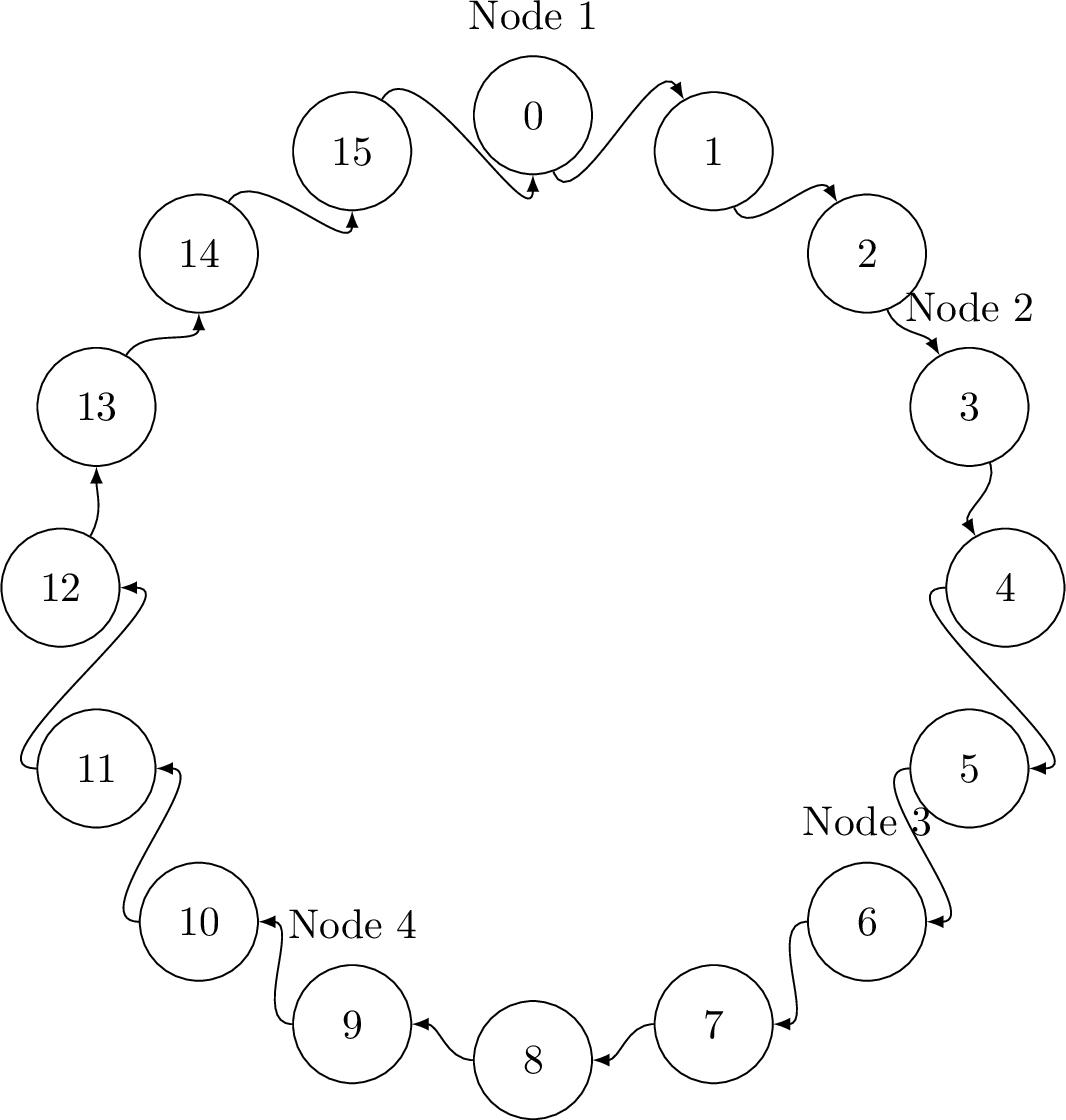
\includegraphics[width=0.45\textwidth]{fig/tex-grapics/chord.pdf.png}
  \caption{Chord Setup}
  \label{fig:chord}
\end{figure}

In diesem Beispiel sind die Knoten (Nodes) im Identifier-Raum wie folgt verteilt: Node 1: ID 0, Node 2: ID 3, Node 3: ID 6, Node 4: ID 9, Node 5: ID 13. Die Idee beim Chord Netz ist, dass der Knoten mit seiner zugeordneten ID verantwortlich ist für einen Bereich größer oder kleiner-gleich seiner eigenen ID. Dies würde für dieses Beispiel bedeuten, wenn der größer-gleich Bereich angenommen wird, dass Node 1 verantwortlich ist für die Keys 0-2, Node 2 verantwortlich für Key 3-5, Node 3 für 6-8, Node 4 für 9 -12 und Node 5 für 13-15. 

\begin{figure}[!ht]
  \centering
  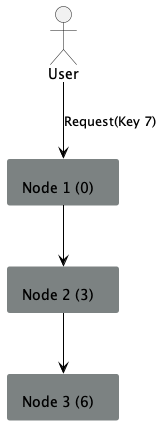
\includegraphics[width=0.15\textwidth]{fig/uml/chord.png}
  \caption{Chord Lookup Example ohne Fingertable}
  \label{fig:chord-lookup}
\end{figure}
Für das Auffinden der Nodes ohne Optimierung wie Fingertables ist nun eine lineare Suche über den Ring notwendig, der in der Graphik~\ref{fig:chord-lookup} beschrieben ist. Eine Suche (Lookup) für den Key 7 wird an dem Node 1 abgesetzt\footnote{Die Anfrage könnte auch an jeden anderen Knoten gestellt werden}. Node 1 ist nicht verantwortlich und leitet an Node 2 weiter, der sie schließlich an Node 3 weiterleitet. Node 3 ist für Key 7 zuständig und wird die angeforderte Ressource zurückgeben.
\\\\
Um den Suchaufwand zu reduzieren, kann zusätzlicher Aufwand für Strukturen betrieben werden, die wir als Fingertables bezeichnen. 
Fingertables sind ein zentraler Bestandteil der Chord-Architektur, die eine effiziente und schnelle Suche nach Schlüsseln und Knoten im Netzwerk ermöglichen. In einem Chord-Netzwerk speichert jeder Knoten eine Fingertable, die Informationen über andere Knoten im Netzwerk enthält. Die Fingertable besteht aus mehreren Einträgen, wobei jeder Eintrag auf einen \enquote{Finger} im Chord-Ring verweist. Die Funktionsweise von Fingertables kann wie folgt beschrieben werden:
\begin{itemize} 
\item Jede Fingertable hat genau $log(n)$ Einträge, wobei n die Anzahl der Knoten im Netzwerk ist.
\item Der i-te Eintrag in der Fingertable eines Knotens n verweist auf den ersten Knoten, der gleich oder nach $(n + 2^{(i-1)}) \mod 2^m$ liegt, wobei m die Anzahl der Bits für den Schlüsselraum ist (z. B. 160 für SHA-1) und i von 1 bis $log(n)$ reicht.
\item Fingertables ermöglichen eine schnelle Suche nach dem verantwortlichen Knoten für einen bestimmten Schlüssel, indem sie den Suchraum bei jedem Schritt effektiv halbieren. Dies wird erreicht, indem sie bei der Suche den nächstbesten Knoten wählen, der näher am gewünschten Schlüssel liegt.
\end{itemize} 

Damit die Fingertables wie erwartet funktionieren, muss sichergestellt werden, dass das Chord-Netzwerk  korrekt initialisiert ist, und alle Knoten müssen ihre Fingertables korrekt aufgebaut haben. Weiter müssen die Knoten im Netzwerk einvernehmliche und konsistente Informationen über die Schlüsselverteilung und die Positionen der anderen Knoten haben. Die Fingertables sollten regelmäßig aktualisiert werden, um Änderungen im Netzwerk - wie das Hinzufügen oder Entfernen von Knoten - zu berücksichtigen und sicherzustellen, dass die Routing-Informationen stets aktuell sind.

Die Verwendung ermöglicht eine effiziente Suche im Chord-Netzwerk, da sie den Suchraum bei jedem Schritt halbieren. Bei einem Lookup wird der am besten passende Knoten aus der Fingertabele ausgewählt, der näher am Ziel liegt, wodurch die Anzahl der Sprünge im Netzwerk verringert wird. Da die Fingertabele $log(n)$ Einträge hat, beträgt die maximale Anzahl der Sprünge, die benötigt werden, um einen Schlüssel zu finden, ebenfalls $log(n)$, dies auf die Hashfunktion zurückzuführen, die diese Verteilung sicherstellt. 
\\\\
Dies ist ein erheblicher Vorteil gegenüber einer naiven linearen Suche, bei der jeder Knoten einzeln überprüft werden müsste, bis der verantwortliche Knoten gefunden ist, was im schlimmsten Fall n Schritte erfordert.

\paragraph{Apache Cassandra Projekt\\\\}
Ein wichtiges Open Source Projekt, das auch der Chord Architektur basiert, ist das Apache Cassandra Projekt, welches hier kurz vorgestellt werden soll. Apache Cassandra ist ein verteiltes, hochverfügbares und skalierbares NoSQL-Datenbanksystem, das sich von der Chord-Architektur inspirieren ließ. Im Gegensatz zum klassischen Chord-Netzwerk hat Cassandra jedoch einige Anpassungen und Erweiterungen vorgenommen, um den Anforderungen moderner verteilter Datenbanksysteme gerecht zu werden. Durch dieses Projekt sollen einige Techniken eingeführt werden, die in der späteren Diskussion nochmal aufgenommen werden sollen. Weiter soll die Ausführung aufzeigen, wie bestehende Ideen über die Zeit Anpassungen und Optimierungen erfahren.

Einige der Anpassungen, die Apache Cassandra im Vergleich zur Chord-Architektur vorgenommen hat, sind:
\begin{itemize} 
\item Partitionierungsstrategie: In Cassandra werden Daten über mehrere Knoten (Nodes) verteilt, indem sie auf Basis eines Partitionsschlüssels, der aus den Eingabedaten extrahiert wird, partitioniert werden. Die Verantwortlichkeit für die Daten wird anhand eines konsistenten Hashing-Algorithmus, ähnlich wie bei Chord, bestimmt.

Die Hauptidee hinter Partitionierungsstrategien besteht darin, den Datenraum in kleinere Partitionen aufzuteilen und diese auf die verschiedenen Knoten im Cluster zu verteilen. Dadurch wird die Last gleichmäßiger auf die Knoten verteilt, und es wird verhindert, dass einige Knoten überlastet werden, während andere Knoten ungenutzt bleiben.

Cassandra verwendet einen Partitionsschlüssel, um den Platz einer Zeile innerhalb einer Tabelle zu bestimmen. Dieser Partitionsschlüssel wird durch einen Partitionierer, wie den Murmur3Partitioner, in einen Token-Wert konvertiert. Der Token-Wert wird dann verwendet, um den verantwortlichen Knoten für diese Partition zu bestimmen.

Sharding ist eine Partitionierungsstrategie, die in verteilten Datenbanksystemen verwendet wird, um Daten auf verschiedene Knoten oder Server aufzuteilen. So wird der gesamte Datensatz in kleinere, handhabbare Teile (Shards) aufgeteilt, wobei jeder Shard auf einem separaten Knoten oder Server gespeichert wird. Sharding kann auf verschiedene Arten implementiert werden, wie z.B.:
\begin{itemize} 
\item Range-based Sharding: Die Daten werden basierend auf einem bestimmten Wertebereich aufgeteilt. Zum Beispiel könnten Kundeninformationen basierend auf der Kunden-ID in unterschiedliche Shards aufgeteilt werden, wobei ein Shard Kunden-IDs von 1 bis 10.000, ein anderer Shard Kunden-IDs von 10.001 bis 20.000 usw. enthält.
\item Hash-based Sharding: Die Daten werden basierend auf einem Hash-Wert aufgeteilt, der aus dem Partitionsschlüssel berechnet wird. In diesem Fall wird der Hash-Wert verwendet, um die Daten gleichmäßig auf die verfügbaren Knoten zu verteilen.
\end{itemize}  
\item Replikationsstrategie: Um Datenverlust zu verhindern und hohe Verfügbarkeit zu gewährleisten, repliziert Cassandra Daten über mehrere Knoten hinweg. Die Anzahl der Replikationen und die Replikationsstrategie können konfiguriert werden. Im Gegensatz zum Chord-Netzwerk, das nur die direkten Nachfolgerknoten für die Replikation verwendet, unterstützt Cassandra verschiedene Replikationsstrategien wie SimpleStrategy und NetworkTopologyStrategy, um eine bessere Kontrolle über die Replikationslogik zu ermöglichen.
\item Datenmodell: Cassandra verwendet ein spaltenorientiertes Datenmodell, das sich von traditionellen relationalen Datenbanken unterscheidet. Das Datenmodell basiert auf einer Tabelle mit einer oder mehreren Partitionen, die wiederum aus einer oder mehreren Zeilen bestehen. Jede Zeile enthält einen eindeutigen Schlüssel und einen oder mehrere Spalten, die die Daten speichern.
\item Gossip-Protokoll: Im Gegensatz zur Chord-Architektur, die Fingertables für das Routing verwendet, verwendet Cassandra ein Gossip-Protokoll für die Kommunikation und den Informationsaustausch zwischen den Knoten. Das Gossip-Protokoll ermöglicht es Knoten, regelmäßig Informationen über ihren Status, ihre Last und die Topologie des Netzwerks auszutauschen.
\item Lese- und Schreibkonsistenz: Cassandra bietet die Möglichkeit, die Konsistenz von Lese- und Schreibvorgängen je nach Anforderungen der Anwendung anzupassen. Die Konsistenz kann auf unterschiedlichen Ebenen gewählt werden, von \enquote{One} (nur ein Knoten muss den Vorgang bestätigen) bis \enquote{All} (alle Replikationsknoten müssen den Vorgang bestätigen). Dies ermöglicht eine bessere Kontrolle über die Trade-offs zwischen Konsistenz, Verfügbarkeit und Performance.
\item Hinted Handoff: Cassandra verwendet ein Mechanismus namens \enquote{Hinted Handoff}, um vorübergehend ausgefallene Knoten zu behandeln. Wenn ein Knoten nicht verfügbar ist, um eine Schreiboperation durchzuführen, speichert ein anderer Knoten einen \enquote{Hint} und stellt die Daten dem ausgefallenen Knoten zur Verfügung, sobald dieser wieder online ist. Dieses Verfahren erhöht die Verfügbarkeit und Fehlertoleranz des Systems.
\item Repair und Anti-Entropy: Im Gegensatz zur Chord-Architektur verfügt Cassandra über Anti-Entropy- und Repair-Mechanismen, um Inkonsistenzen zwischen Replikationsknoten zu erkennen und zu beheben. Cassandra verwendet Merkle Trees, um Unterschiede zwischen Replikationen effizient zu erkennen und bei Bedarf Daten synchronisieren.
\end{itemize}
\paragraph{Anti-Entropy (kurz)\\\\}
Anti-Entropy ist ein Mechanismus in verteilten Systemen, der dazu dient, die Konsistenz und Stabilität von Daten über mehrere Knoten (Nodes) hinweg sicherzustellen. In einem verteilten System arbeiten mehrere unabhängige Knoten zusammen, um eine gemeinsame Aufgabe zu erfüllen, wie zum Beispiel die Speicherung und Verwaltung von Daten. Diese Knoten können jedoch aufgrund von Netzwerkverzögerungen, Fehlern oder Abstürzen inkonsistente Daten enthalten. Diese Verfahren werden in einem späteren Kapitel nochmals genauer betrachtet. 
\\\\
Anti-Entropy-Prozesse sorgen dafür, dass die Daten auf den verschiedenen Knoten synchronisiert und konsistent bleiben. Sie verwenden Replikations- und Synchronisationsverfahren, um sicherzustellen, dass alle Knoten dieselben Daten enthalten.

\label{Woche06}
\end{document}
